\chapter{Experiments}\label{cap.experiments}


In this chapter we characterize the quality of each module and explain the validation experiments of our solution. Also, we explain several alternatives that we considered for each module.



\section{Detection experiments}\label{valdiation:det}


For the final choice of the detector to be included in our application we compared sevveral detectors studied in the theoretical review \ref{trackingBounding} and we tested them on the \textit{MOT16} dataset. In the figure \ref{experimDet1} we can observe the ROC curves of different detectors.



\begin{figure}[H]
\centering         
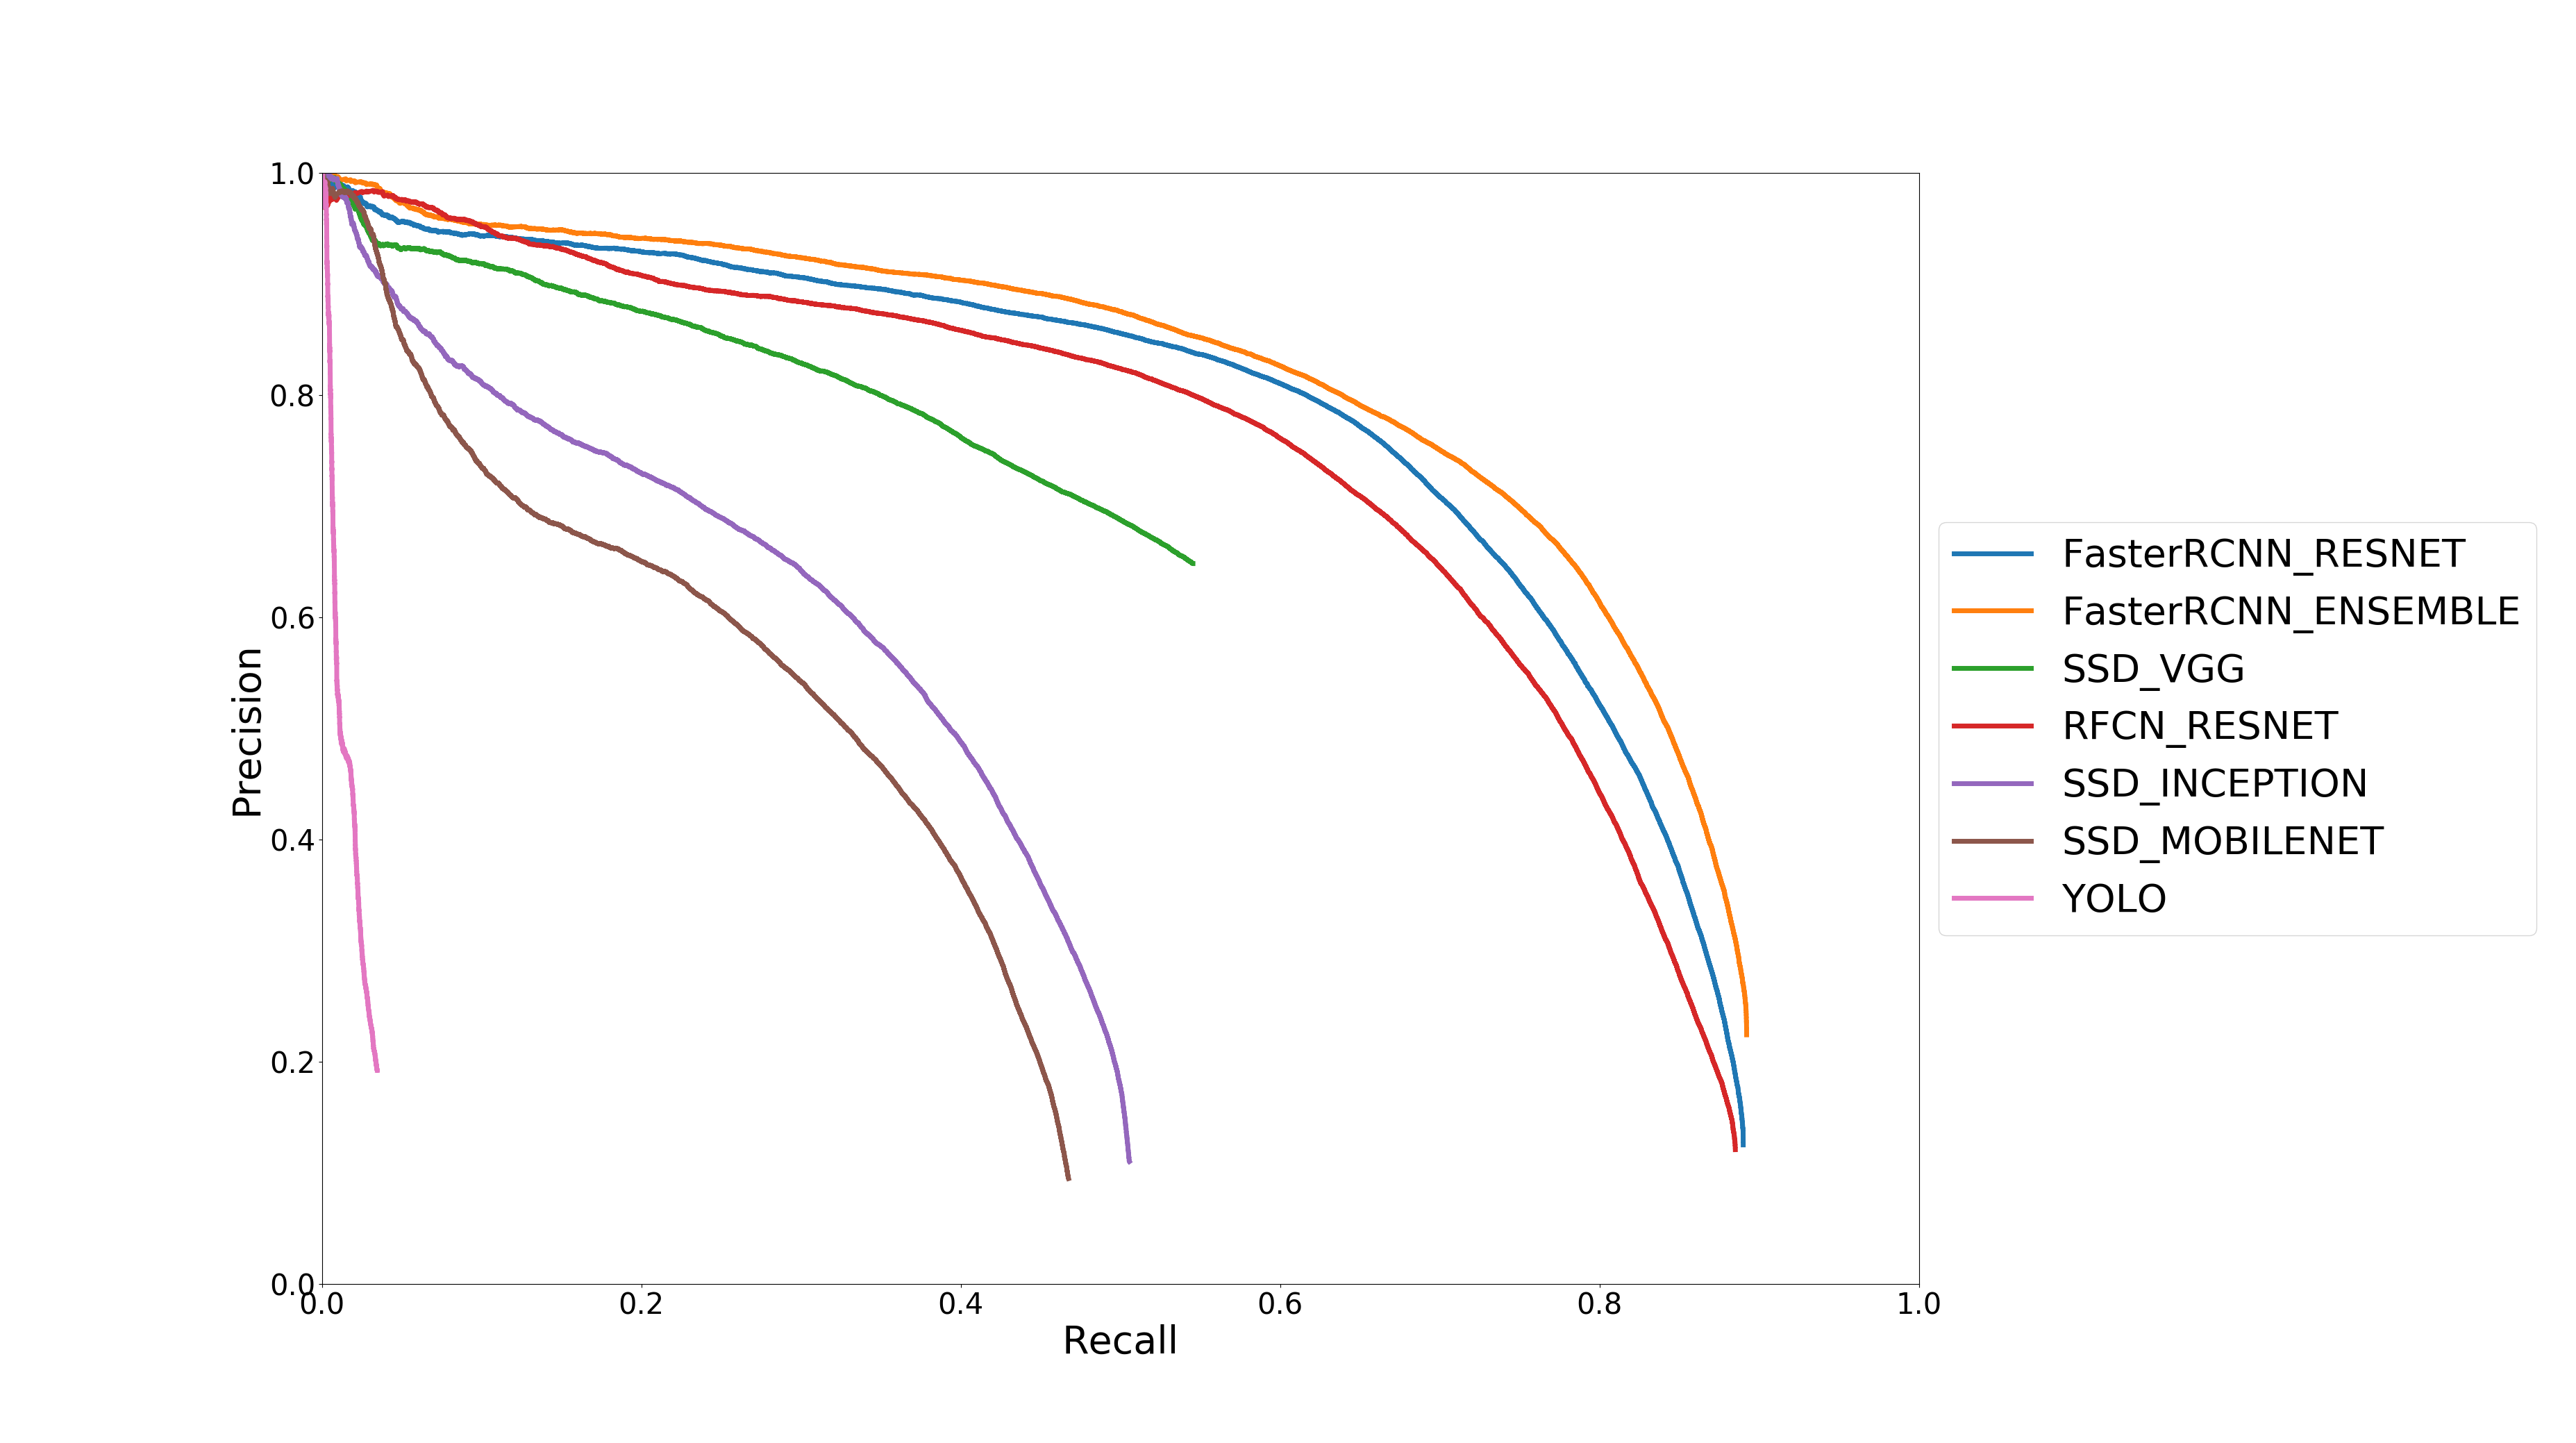
\includegraphics[width=0.9\linewidth]{evaluacionObject/dadas.png}
\caption{ROCs curves on the MOT16 dataset.} \label{experimDet1}
\end{figure}

In the figure \ref{experimDet2} we can observe the mean average precision against the time consumption.


\begin{figure}[H]
\centering         
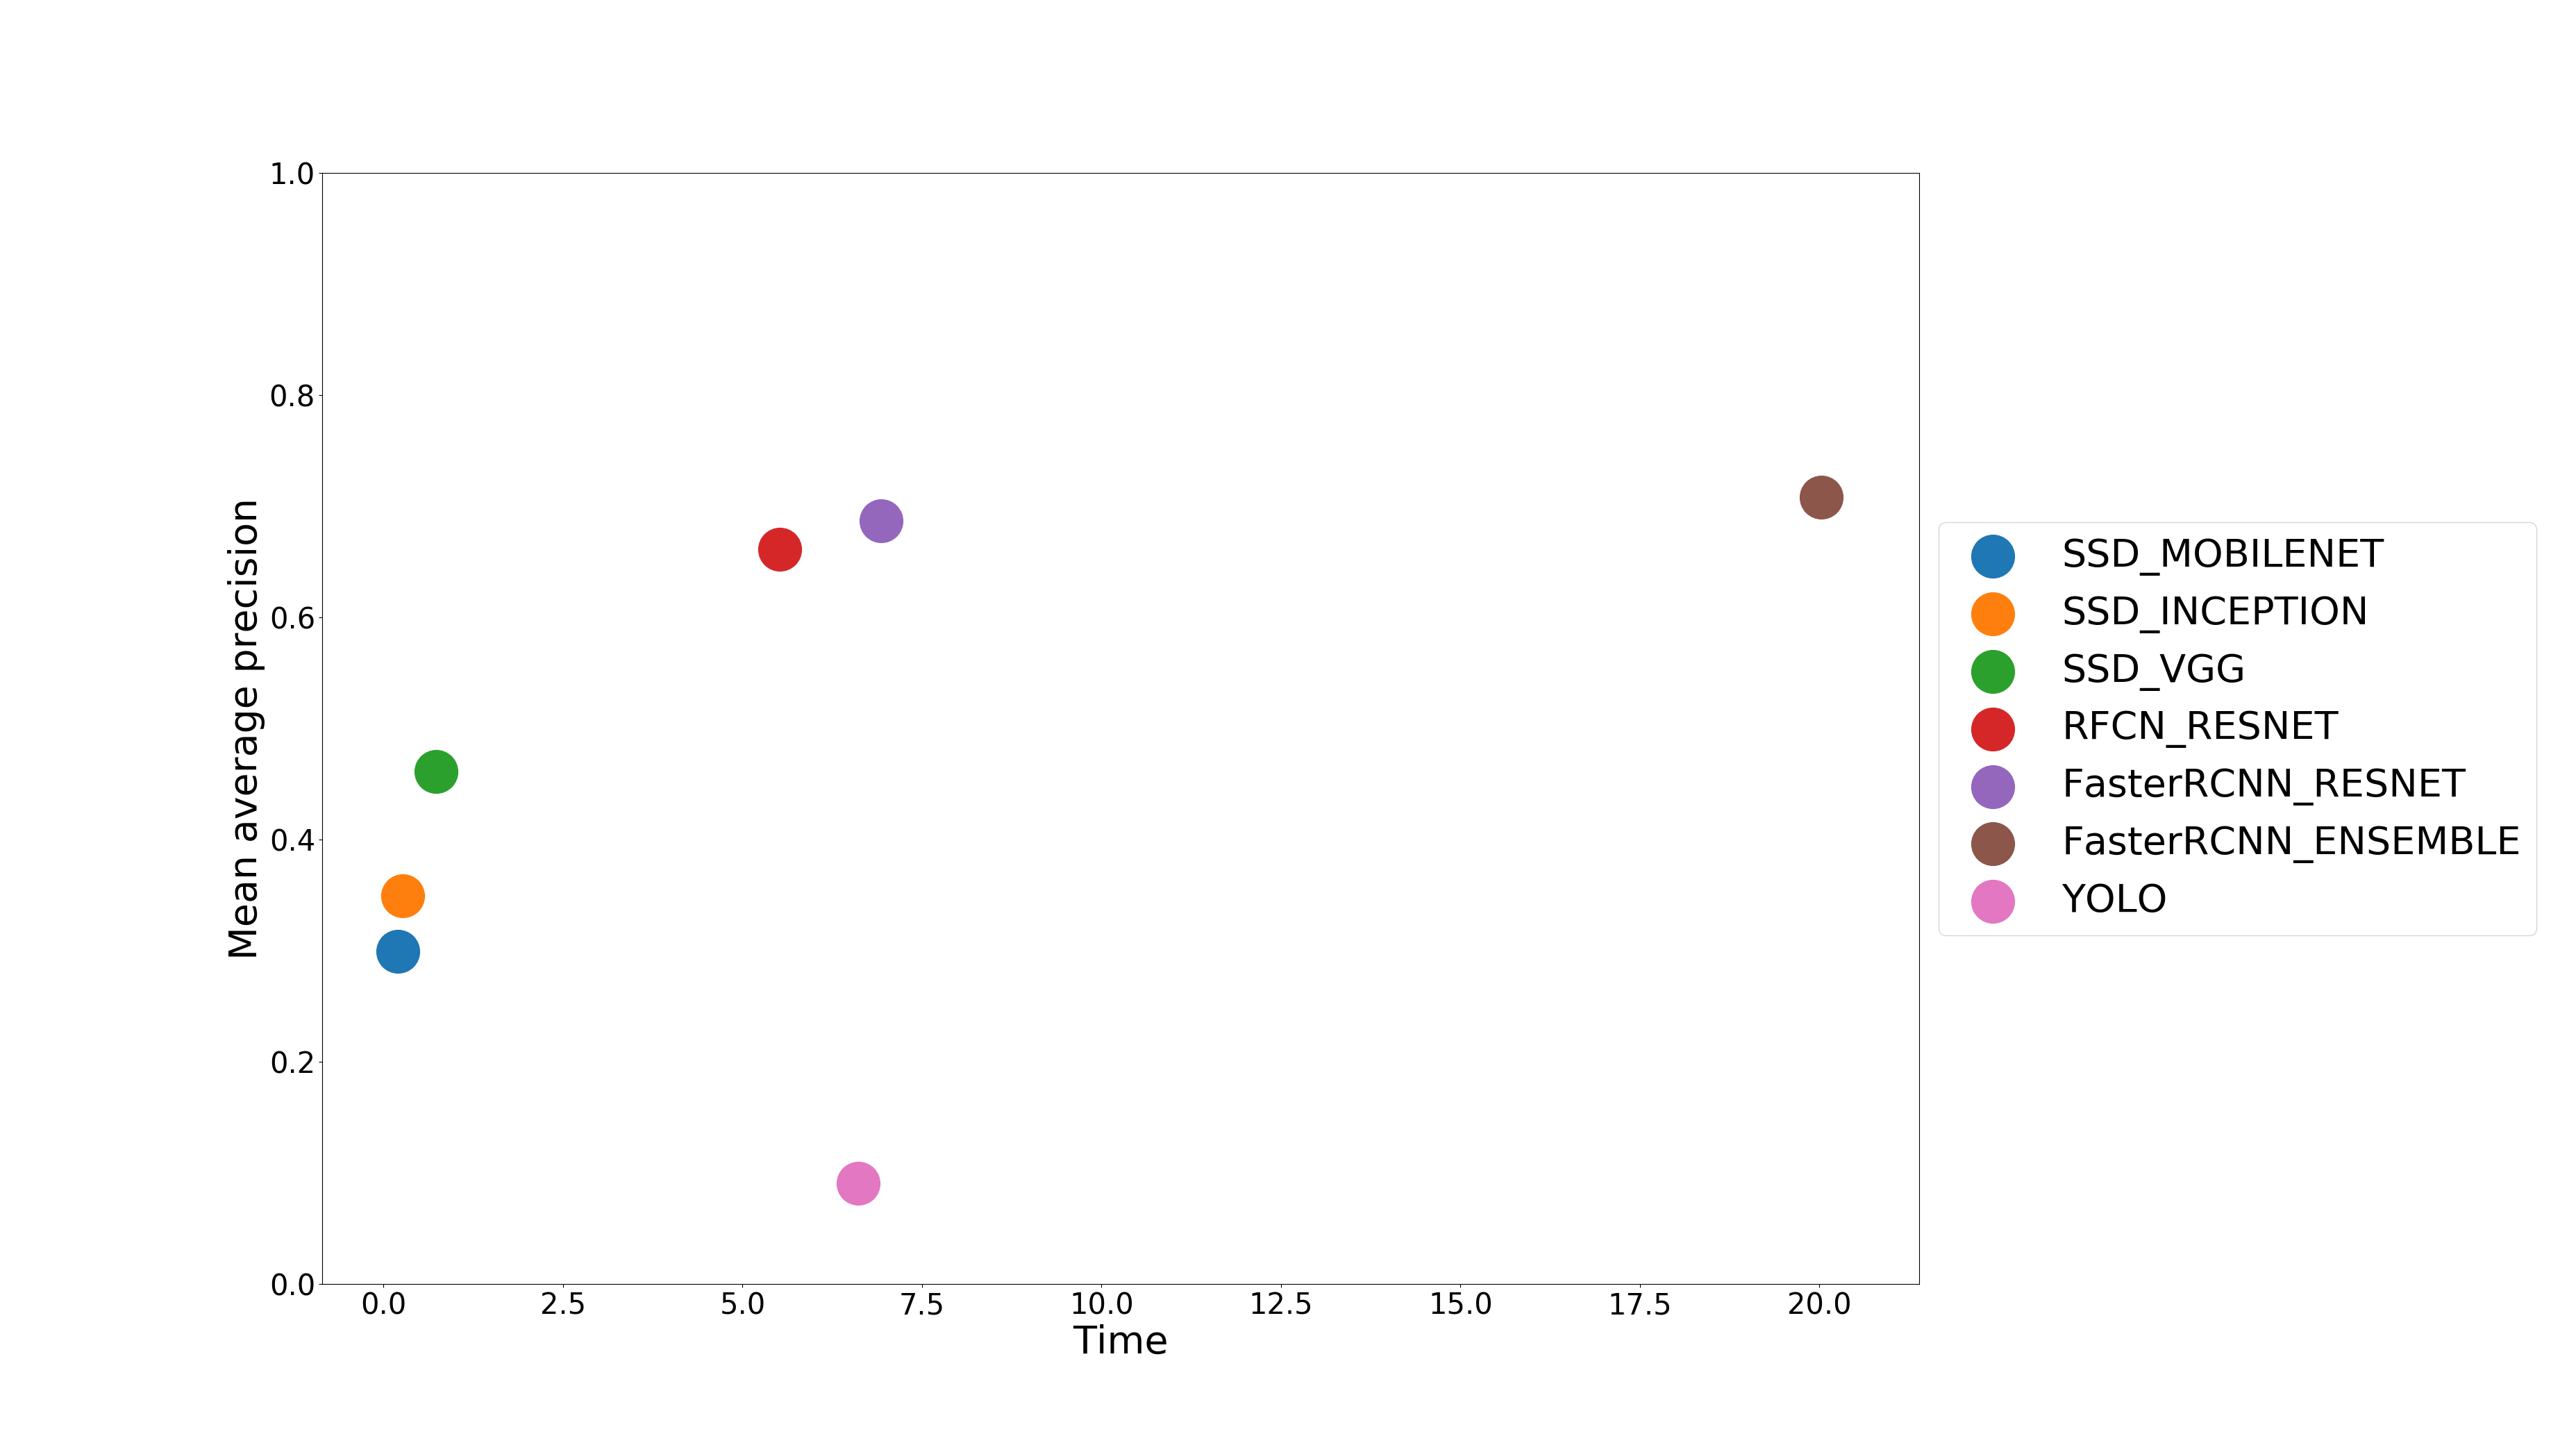
\includegraphics[width=0.9\linewidth]{evaluacionObject/meanAverage2.png}
\caption{Mean average precision against time.} \label{experimDet2}
\end{figure}

With this information we can summarize the conclusions of the study of the detectors:

\begin{itemize}

\item \textbf{Faster-RCNN}, we used the TensorFlow implementation \cite{tensorObjectdte}, the original code required a Nvidia GPU. This repository includes the Faster-RCNN model with ResNet as feature extraction and the ensemble model compound by Inception-ResNet. It scores $0.6872$ and $0.7081$ average precision with a time consumption of  $6.93$ and  $20.029$ seconds respectively. These are the highest accuracy value obtained in this comparison, but also the slowest.



\item \textbf{R-FCN}, the original code is not publicly available. We used the TensorFlow implementation \cite{tensorObjectdte}. It scores $0.6614$ average precision and $5.514$ seconds. This accuracy value is similar to the previous one but is slow.


\item \textbf{YOLO}, we used the original and it scores $0.09$ average precision on the dataset, it takes $6$ seconds per image \cite{yoloDark}. It takes too time for this awful score. According to the theory \ref{trackingBounding} this is the fastest detector, but it does not optimized to run on cpu.

\item \textbf{PVANET}, the code is not publicly available.

\item \textbf{SSD}, we tested several feature extractors with this model. Their scores are the following: the SSD model with VGG as feature extractor, it scores $0.4612$ average precision and takes $0.73$ seconds; SSD with Inception as feature extractor it scores $0.3499$ average precision and takes $0.73$ seconds; and SSD with MobileNet as feature extractor it scores $0.2995$ average precision and  takes $0.198$ seconds. The original code \cite{ssdCode2} is not optimized for CPU execution, it takes about $3.5$ seconds and the Caffe framework does not allow to run it in a multithreading way, so we discarded it. The VGG version comes from a particular developer \cite{ssdCode} and the Inception and MobileNet from TensorFlow organization \cite{tensorObjectdte}.


\end{itemize}

According to these results the object detector with the best balance between precision and time consumption is the SSD detector with VGG feature extractor. Detectors like SSD-Inception and SSD-MobileNet are really fast but their performance is $23 \%$ lower than the SSD with VGG. In contrast, RFCN is more accurate but it takes $700 \%$ more time than SSD with VGG.


The MOT organization provides a set of detections, they include FasterRCNN, DPM v5, and SPD \cite{spd}. We were not able to reproduce their results, because we can not access to the original code. In the figure \ref{experimDet3} we can observe those detections.




\begin{figure}[H]
\centering         
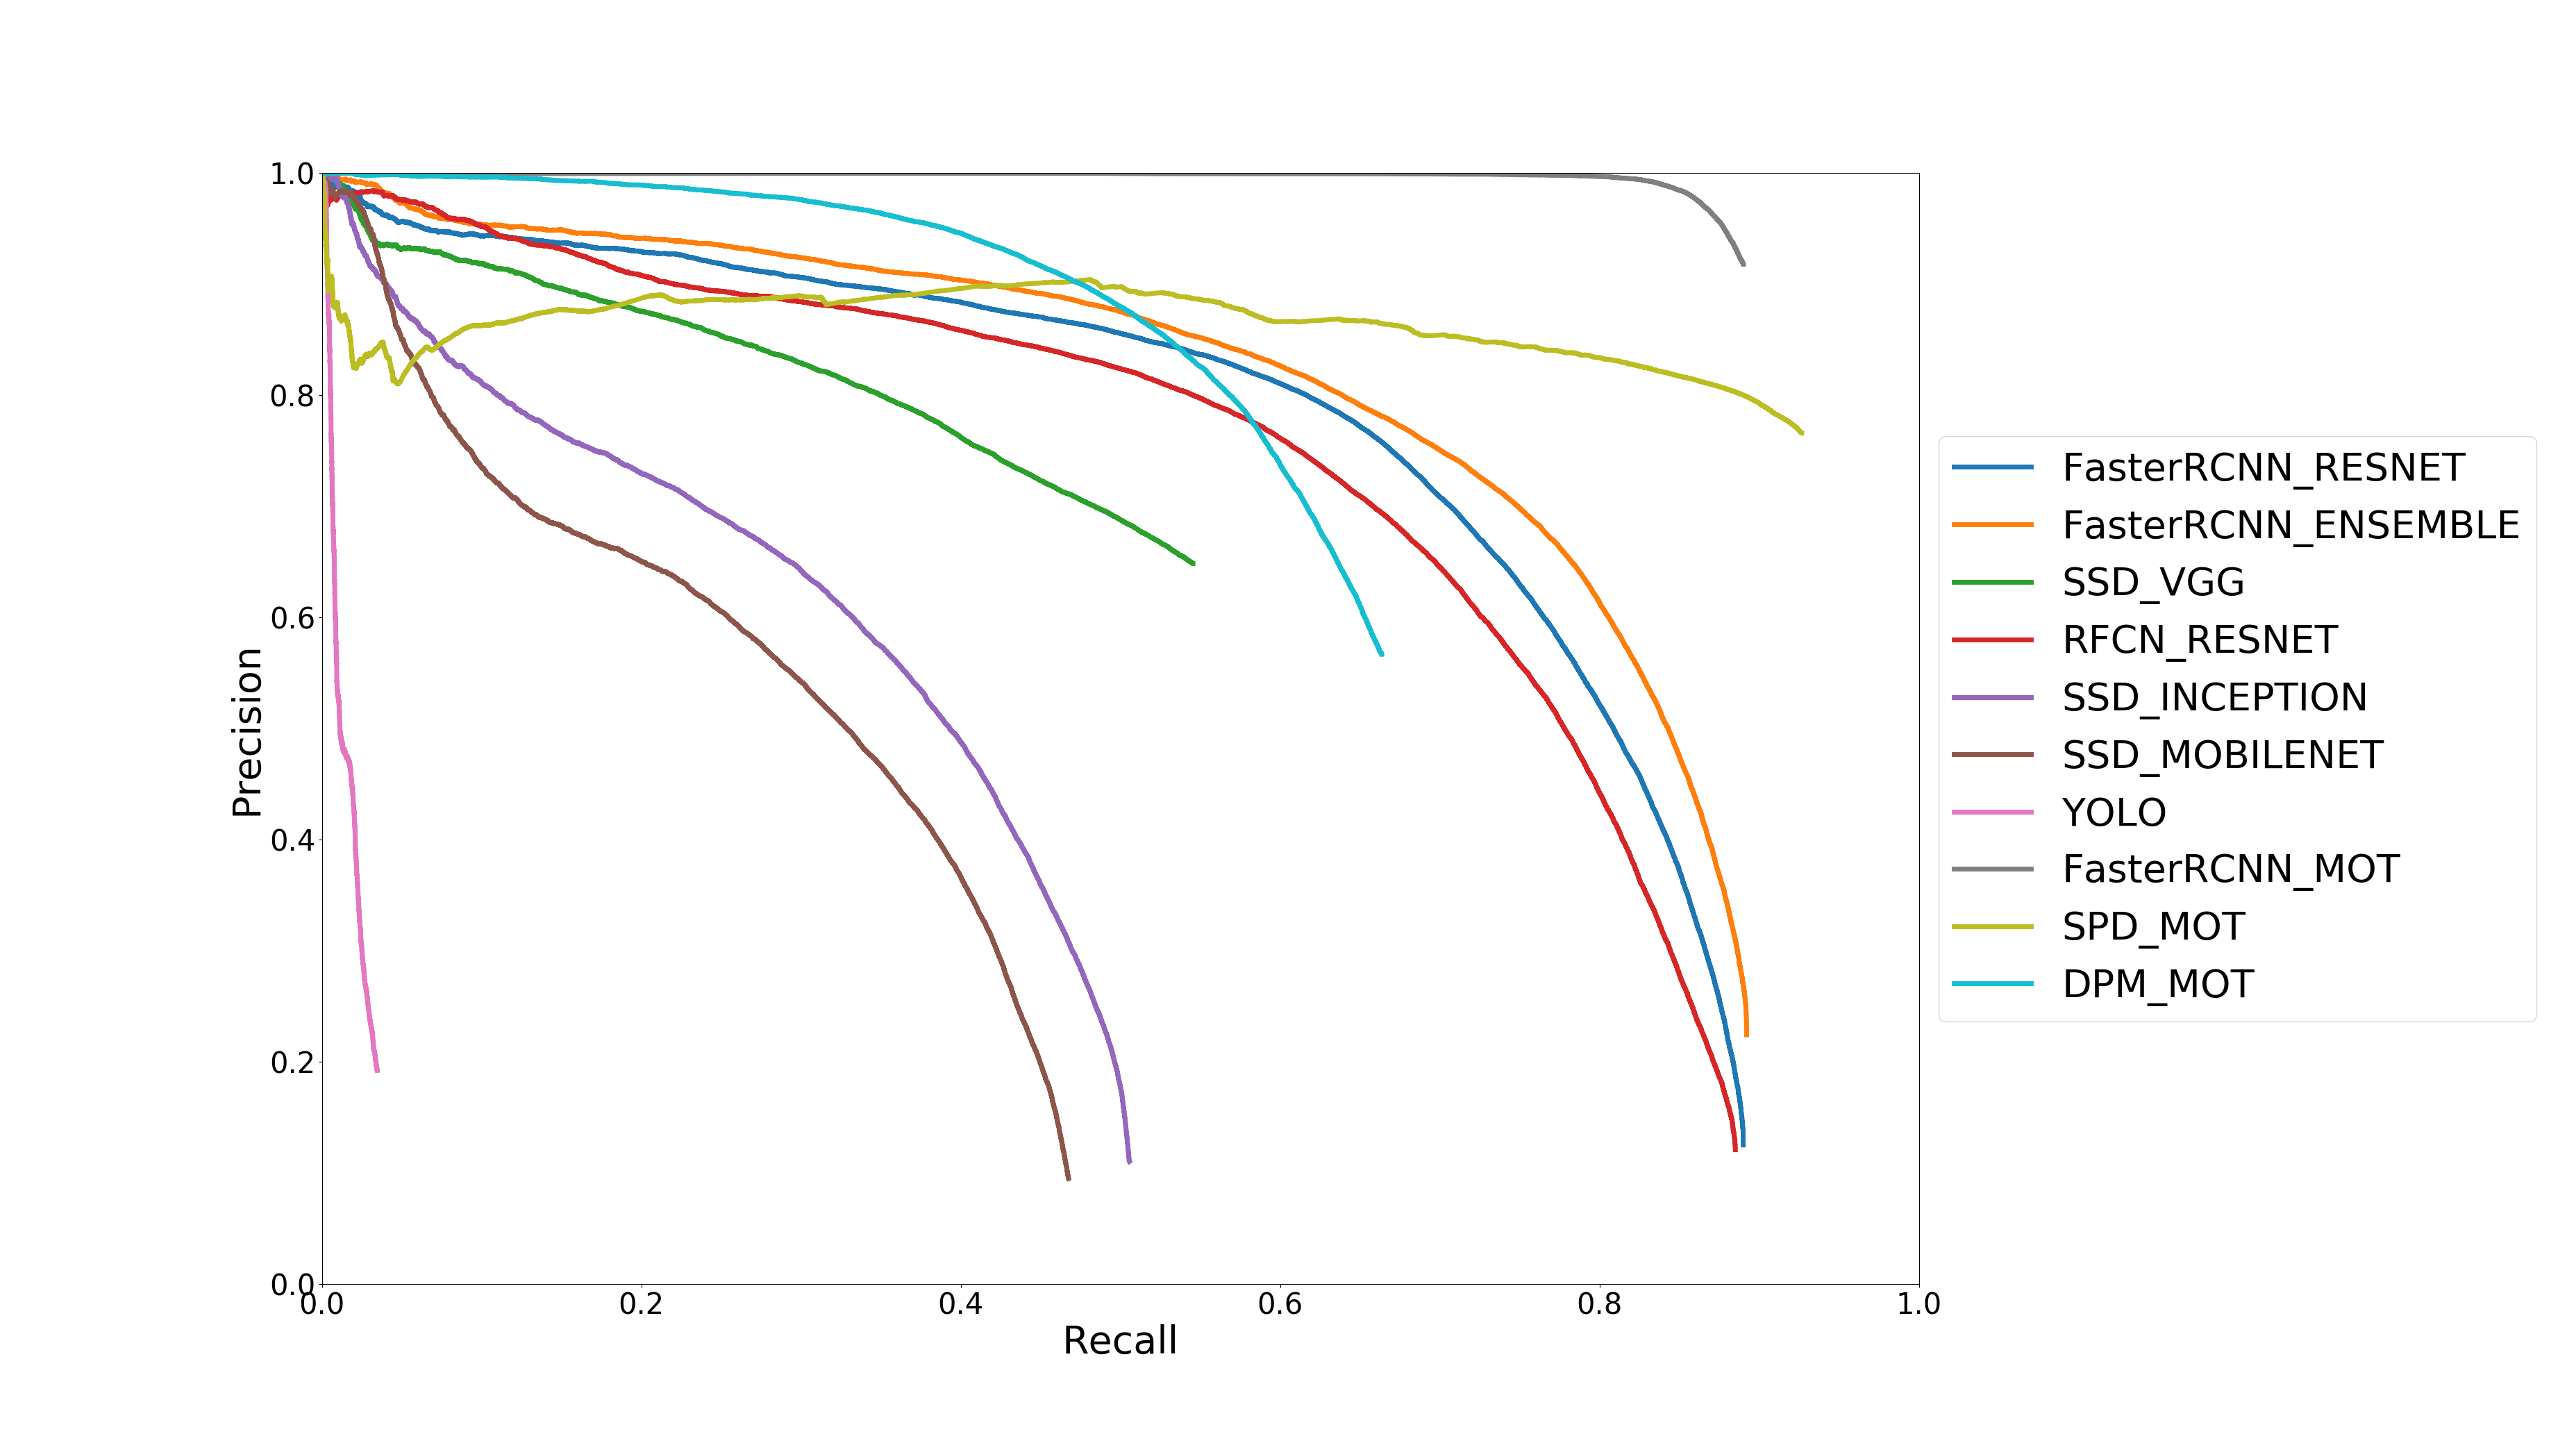
\includegraphics[width=0.9\linewidth]{evaluacionObject/motdetece.png}
\caption{ROCs curves on the MOT16 dataset.} \label{experimDet3}
\end{figure}


\section{Feature-based tracking experiments}\label{trackingsesad}



We started developing our feature-based tracking module with simple artificial objects like the one in the figure \ref{trs}. As soon we had got expertise we shift to much complex models like people. Finally, the last version of the tracking module was inspired by the well-known tracking algorithm \textit{MedianFlow} by Zalal et al\cite{medianFlow} with its correspondent implementation in Python\cite{medianFlowPython}.
 

\begin{figure}[H]
\centering         
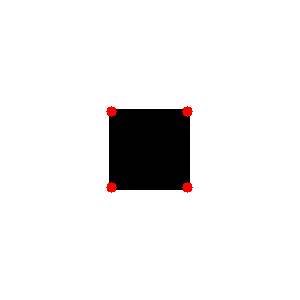
\includegraphics[width=6cm]{tracker/scale1points.png}
\caption{Artificial object to start tracking.} \label{trs}
\end{figure}





%The tracking module is inspired by the well-known tracking algorithm \textit{MedianFlow} by Zalal et al\cite{medianFlow} with its correspondent implementation in Python\cite{medianFlowPython}.

This tracking uses matching based on the optical flow, explained in section \ref{matchi}. It computes the new position through gradient descent in several frames. We assume that the motion is pure translational. As we can observe in the sequences of frames \ref{experiTrack1} of the dataset, the typical pedestrian moves in translation in the image plane, so this assumption may hold for most of the people appearing in the scene.

\begin{figure}[H]
\centering         
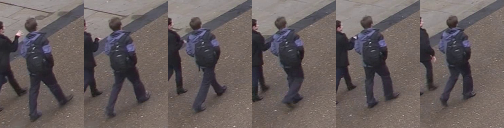
\includegraphics[width=0.9\linewidth]{changeCamera/trrasls.png}
\caption{Sequence of translational movement.} \label{experiTrack1}
\end{figure}

In contrast to the previous figure, we can observe the figure \ref{experiTrack2} where the assumption of translation motion is not fulfilled ( this sequences does not belong to the used dataset, only showed to contrast the previous idea) and a translational assumption will fail. The car in that image significantly rotates in the same scenario, in addition with a traslation.

\begin{figure}[H]
\centering         
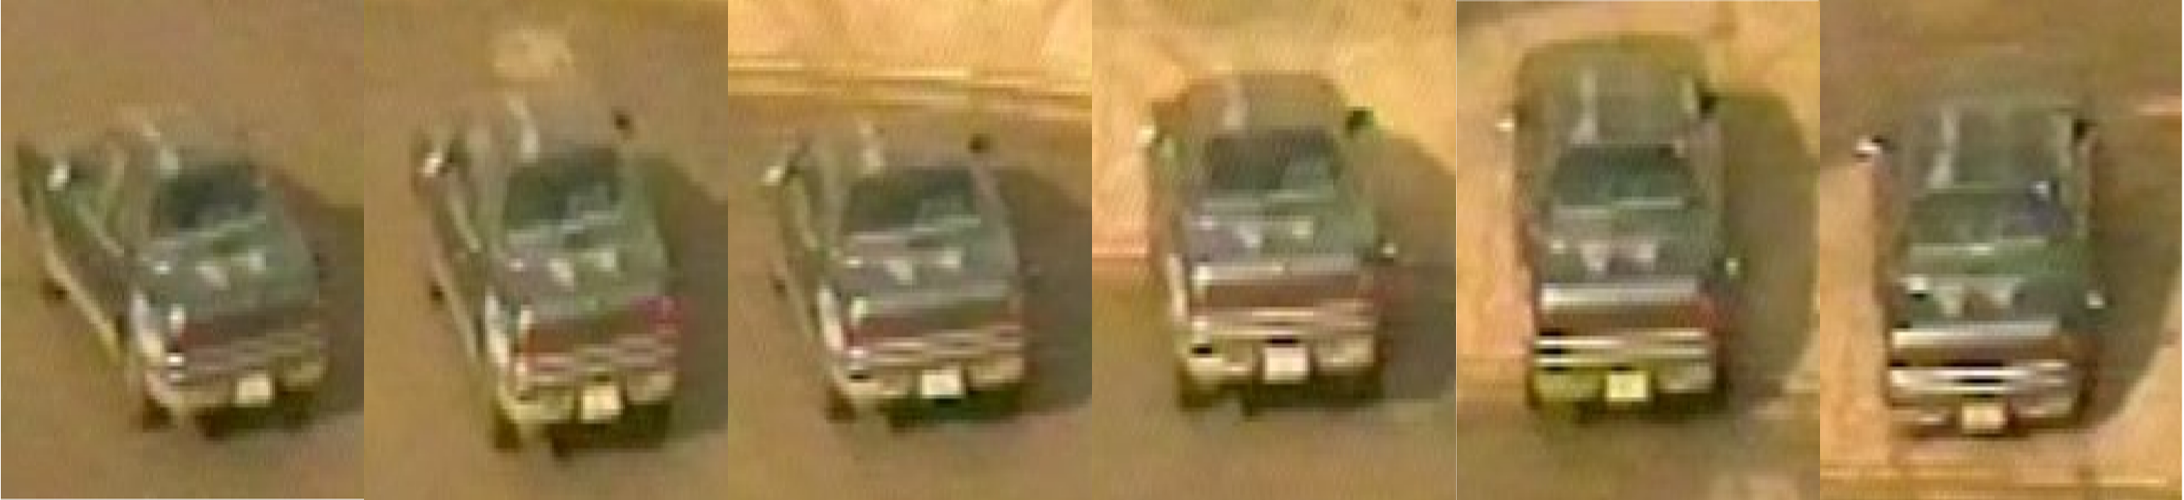
\includegraphics[width=0.9\linewidth]{changeCamera/out2.png}
\caption{Sequence of no translational movement.} \label{experiTrack2}
\end{figure}

We tested other tracking algorithms, like MeanShift, but we discarded it due to its problems to track pedestrians in a messy background.






\subsection{Feature extraction improvement}\label{exper:validation}

The strength of the further processing greatly depends on the quality and quantity of features detected in the images. In order to enhance the general performance, we apply some prepreprocessing to the images. We tried several preprocessings techniques like sharpening, image contrast, median filter, and equalization. In \ref{experiTrack3}, we can observe the relation between number of points extracted and time consumption of those techniques.




\begin{figure}[H]
\centering         
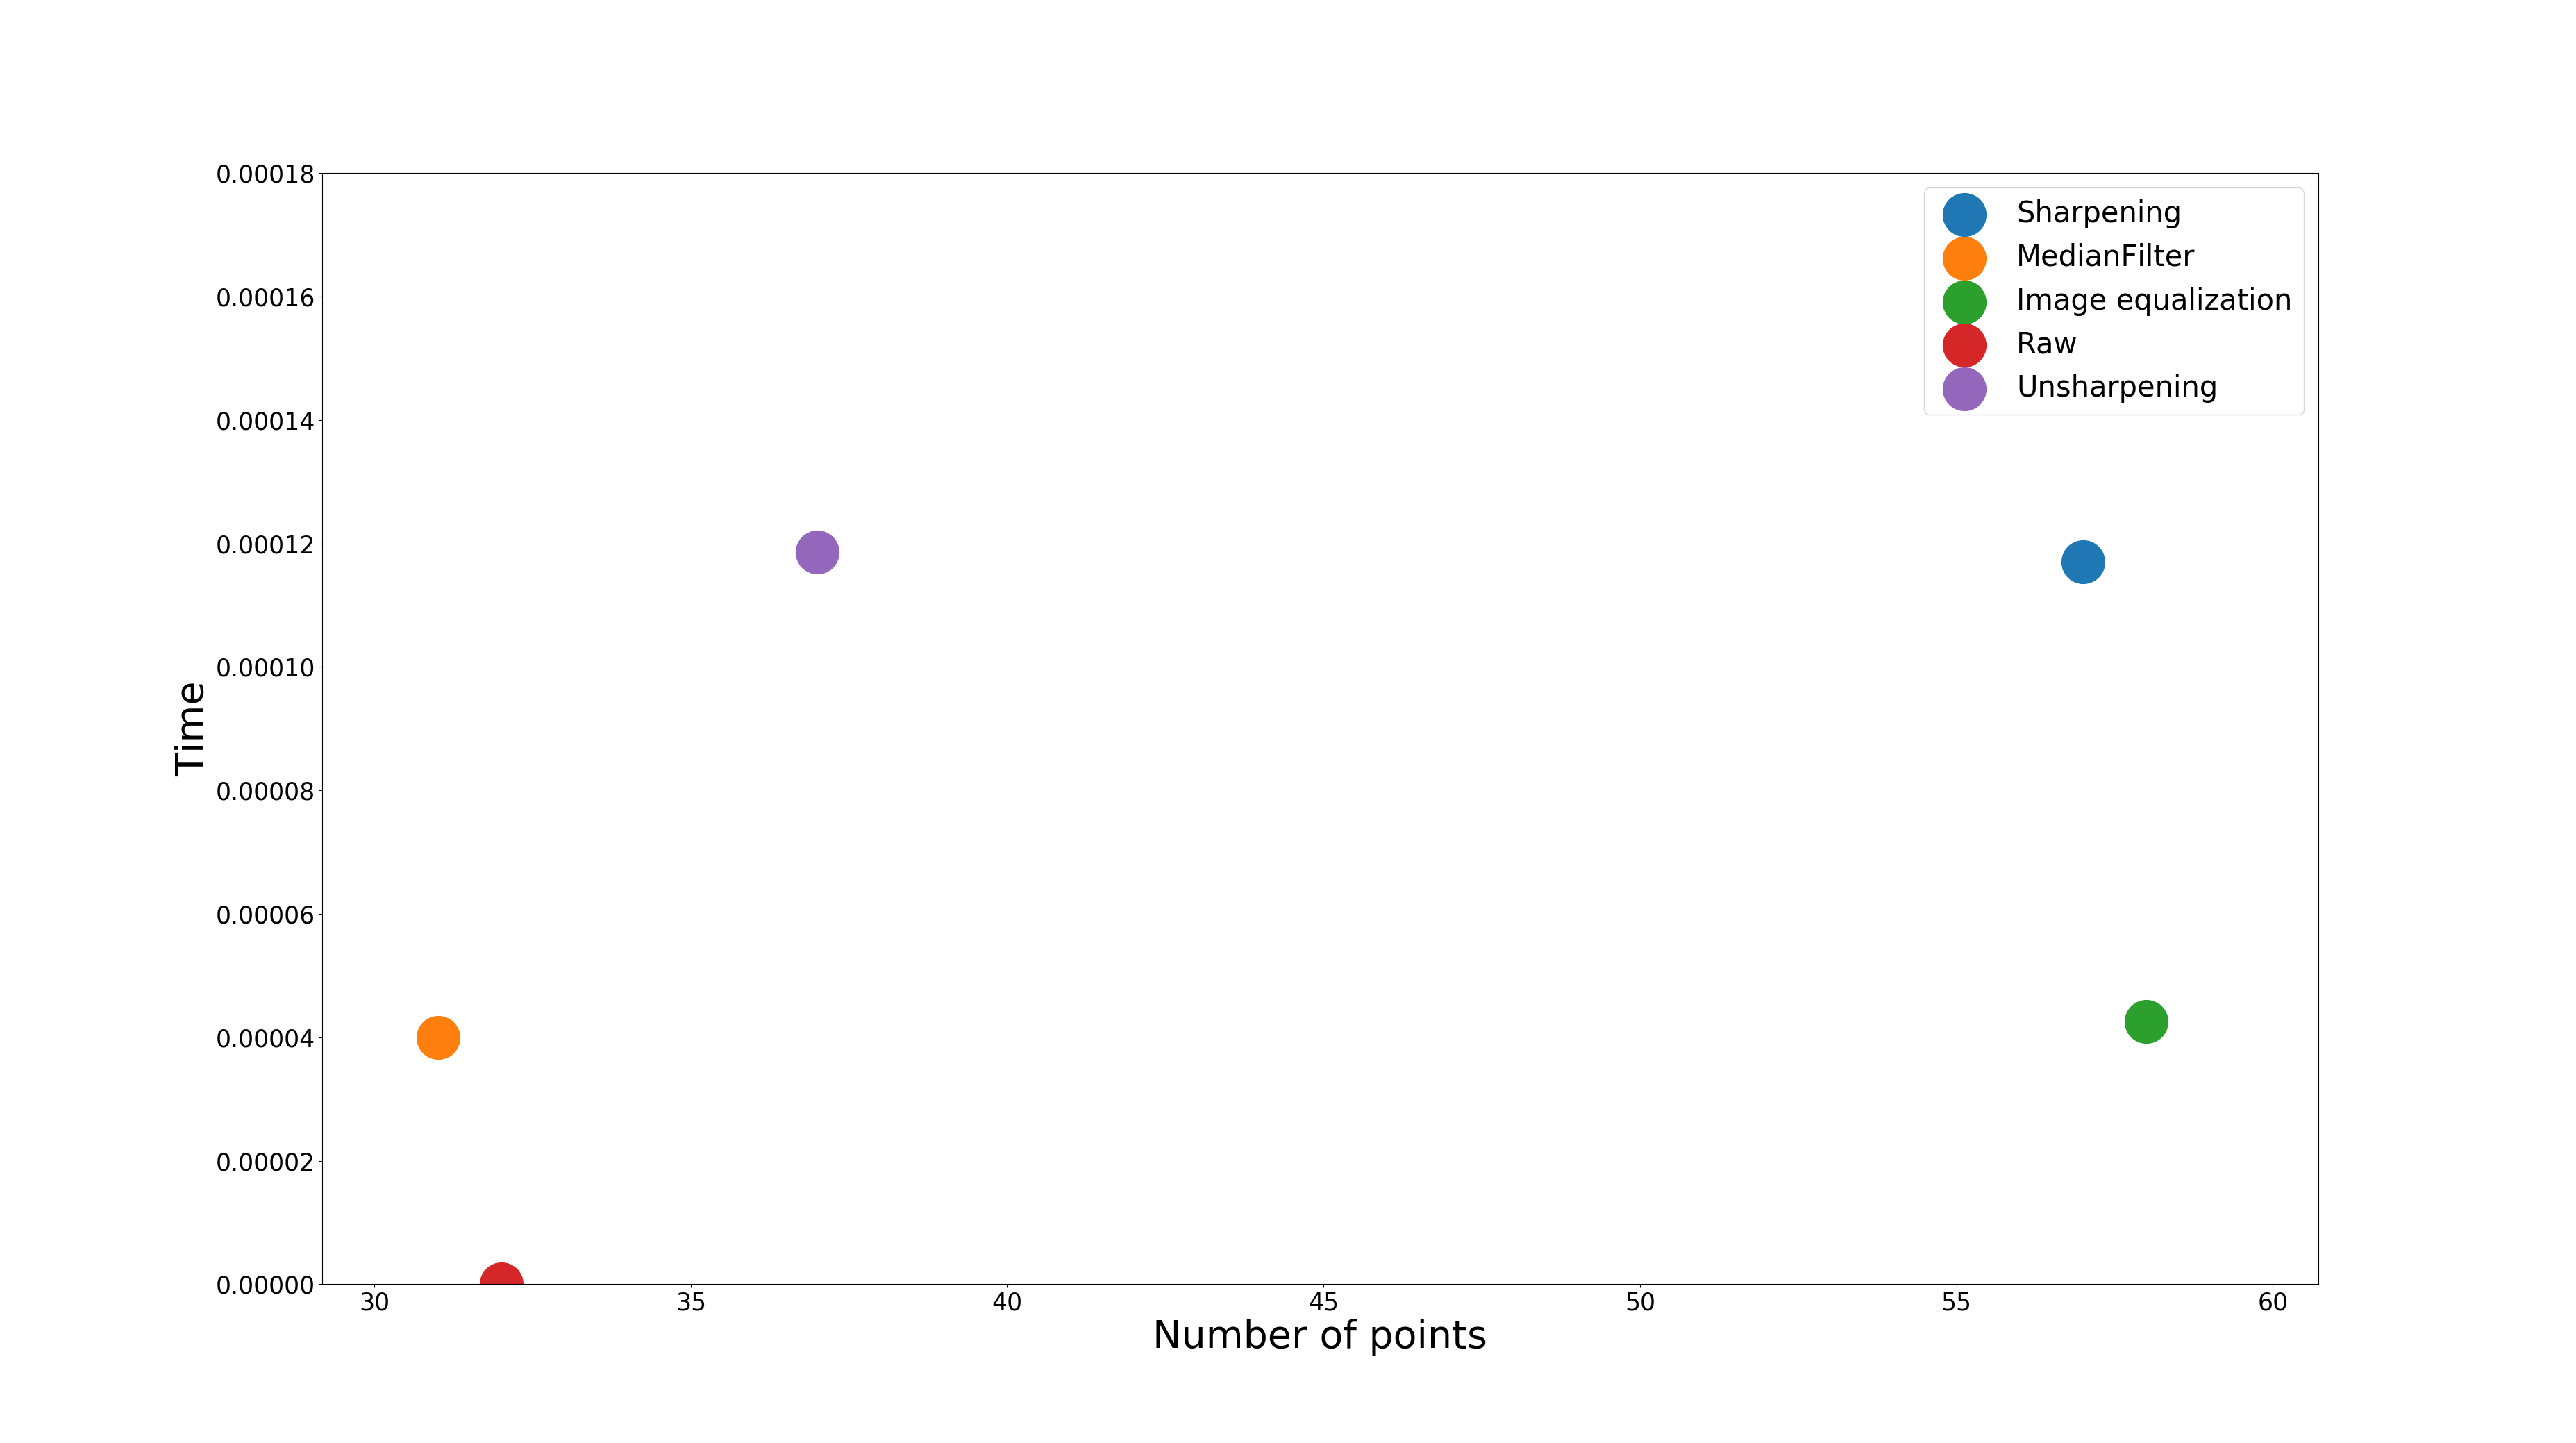
\includegraphics[width=0.9\linewidth]{tracker/preprocesing.png}
\caption{Plot of different image preprocessing techniques.} \label{experiTrack3}
\end{figure}

With this experiment, we realized that the best preprocessing in terms of speed and number of points, is to equalize the image. The computation is really simple, it only consists of equalizing an histogram and applying that transformation to the image. It increases over $ 55 \%$ the number points in comparison to not applying it to the raw image. In the figure \ref{experiTrack4} we can observe the different number of features in the raw and in the equalized image.

\begin{figure}[H]
		
\centering

\subfigure[]{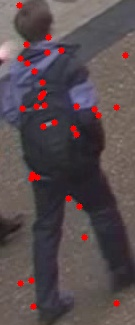
\includegraphics[width=3cm]{implementation/pointsSIN_EQU.jpg}}
\subfigure[]{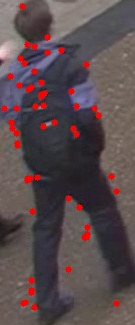
\includegraphics[width=3cm]{implementation/pointsEQU.jpg}}\\
\caption{Comparison between feature extraction on raw (a) and equalized image (b).}
\label{experiTrack4}
\end{figure}


\subsection{Matching module}

We used the Lukas-Kanade algorithm to get the displacement of the features but we implemented the same method used in \cite{medianFlow} too. The proposed method is based on so called forward-backward consistency assumption. This assumes in that correct tracking should be independent of the direction of time-flow.
Algorithmically, the assumption is exploited as follows. First, a tracker produces a trajectory by tracking the point \textit{forward} in time. Second, the point location in the last frame initializes a validation trajectory. The validation trajectory is obtained by \textit{backward} tracking from the last frame to the first one. Third, the two trajectories are compared and if they differ significantly, the forward trajectory is considered as incorrect. 

Figure \ref{experiTrack5} illustrates the method when tracking a point between two images. Point number $1$  is visible in both images and the tracker is able to localize it correctly. Tracking this point forward or backward results in identical trajectories. On the other hand, point number $2$ is not visible in the right image and the tracker localizes a different point. Tracking this point backward ends in a different location than the original one.

\begin{figure}[H]
		
\centering

\subfigure[Image forward-backward.]{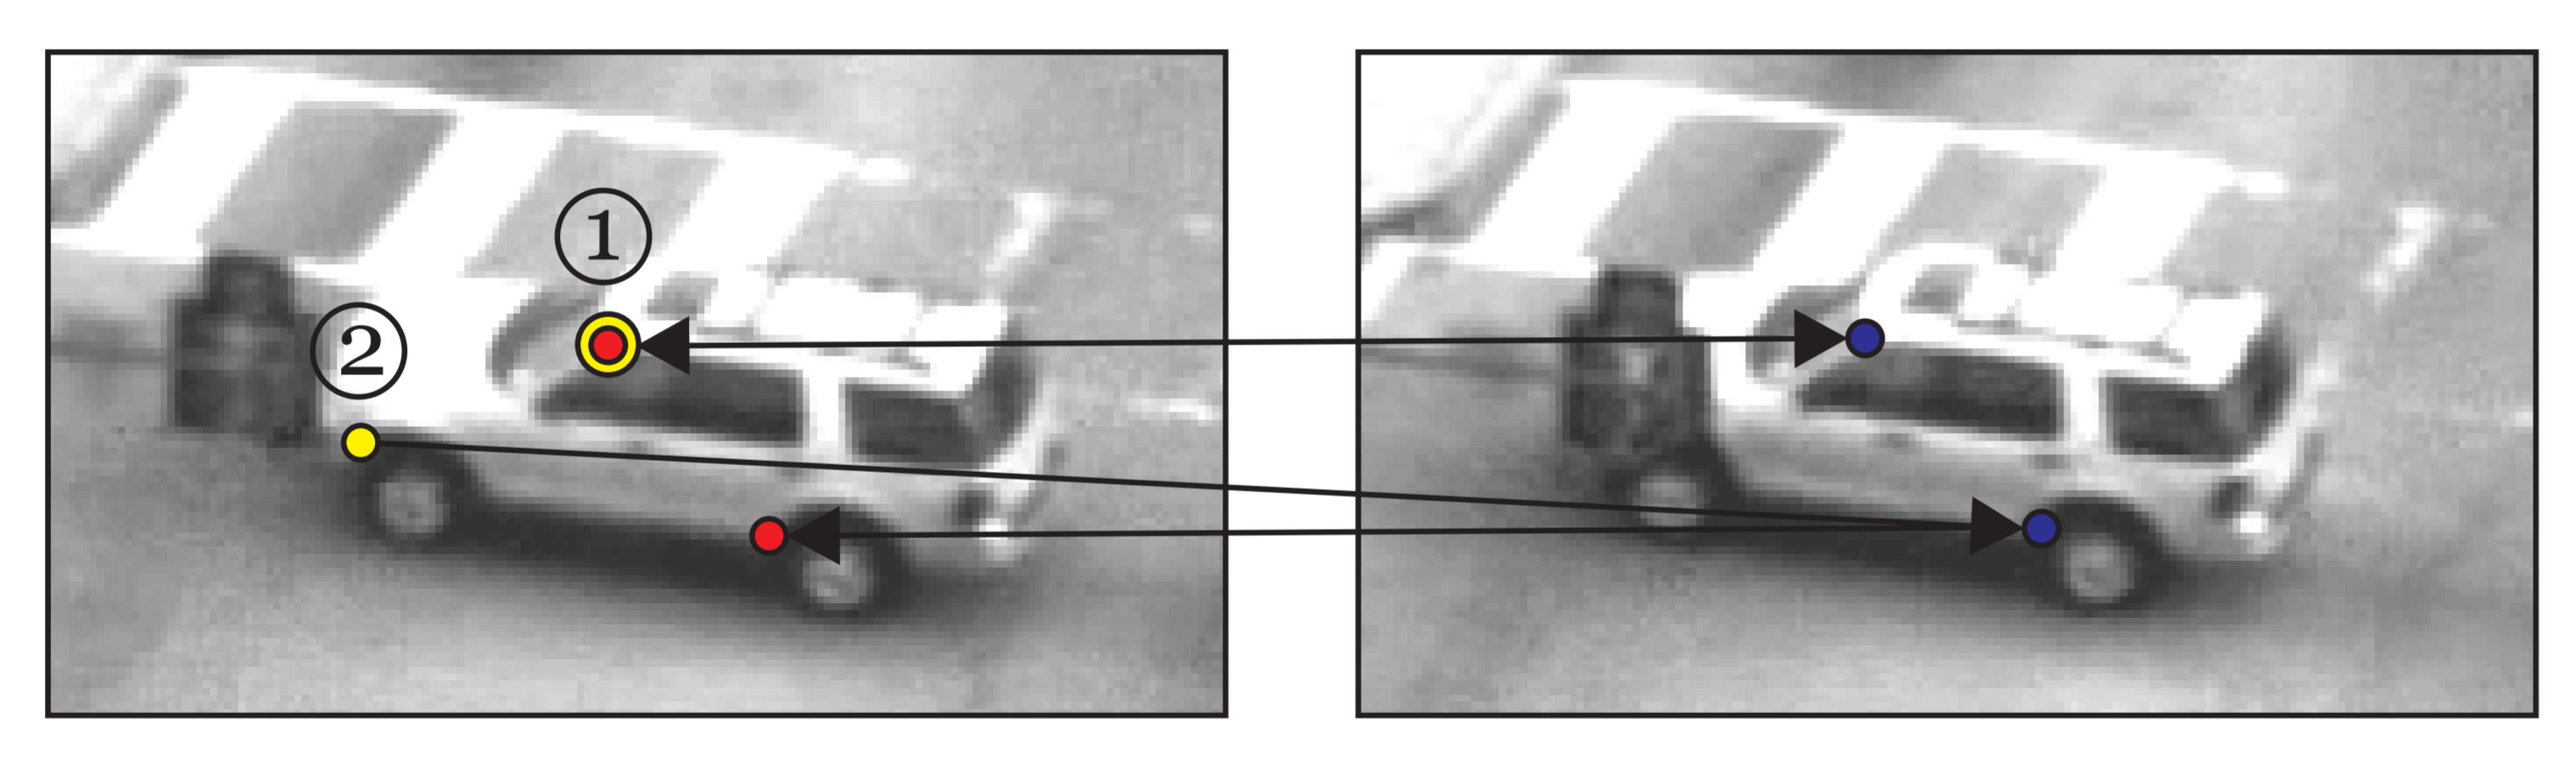
\includegraphics[width=7cm]{tracker/forwardBack.png}}
\subfigure[Scheme forward-backward.]{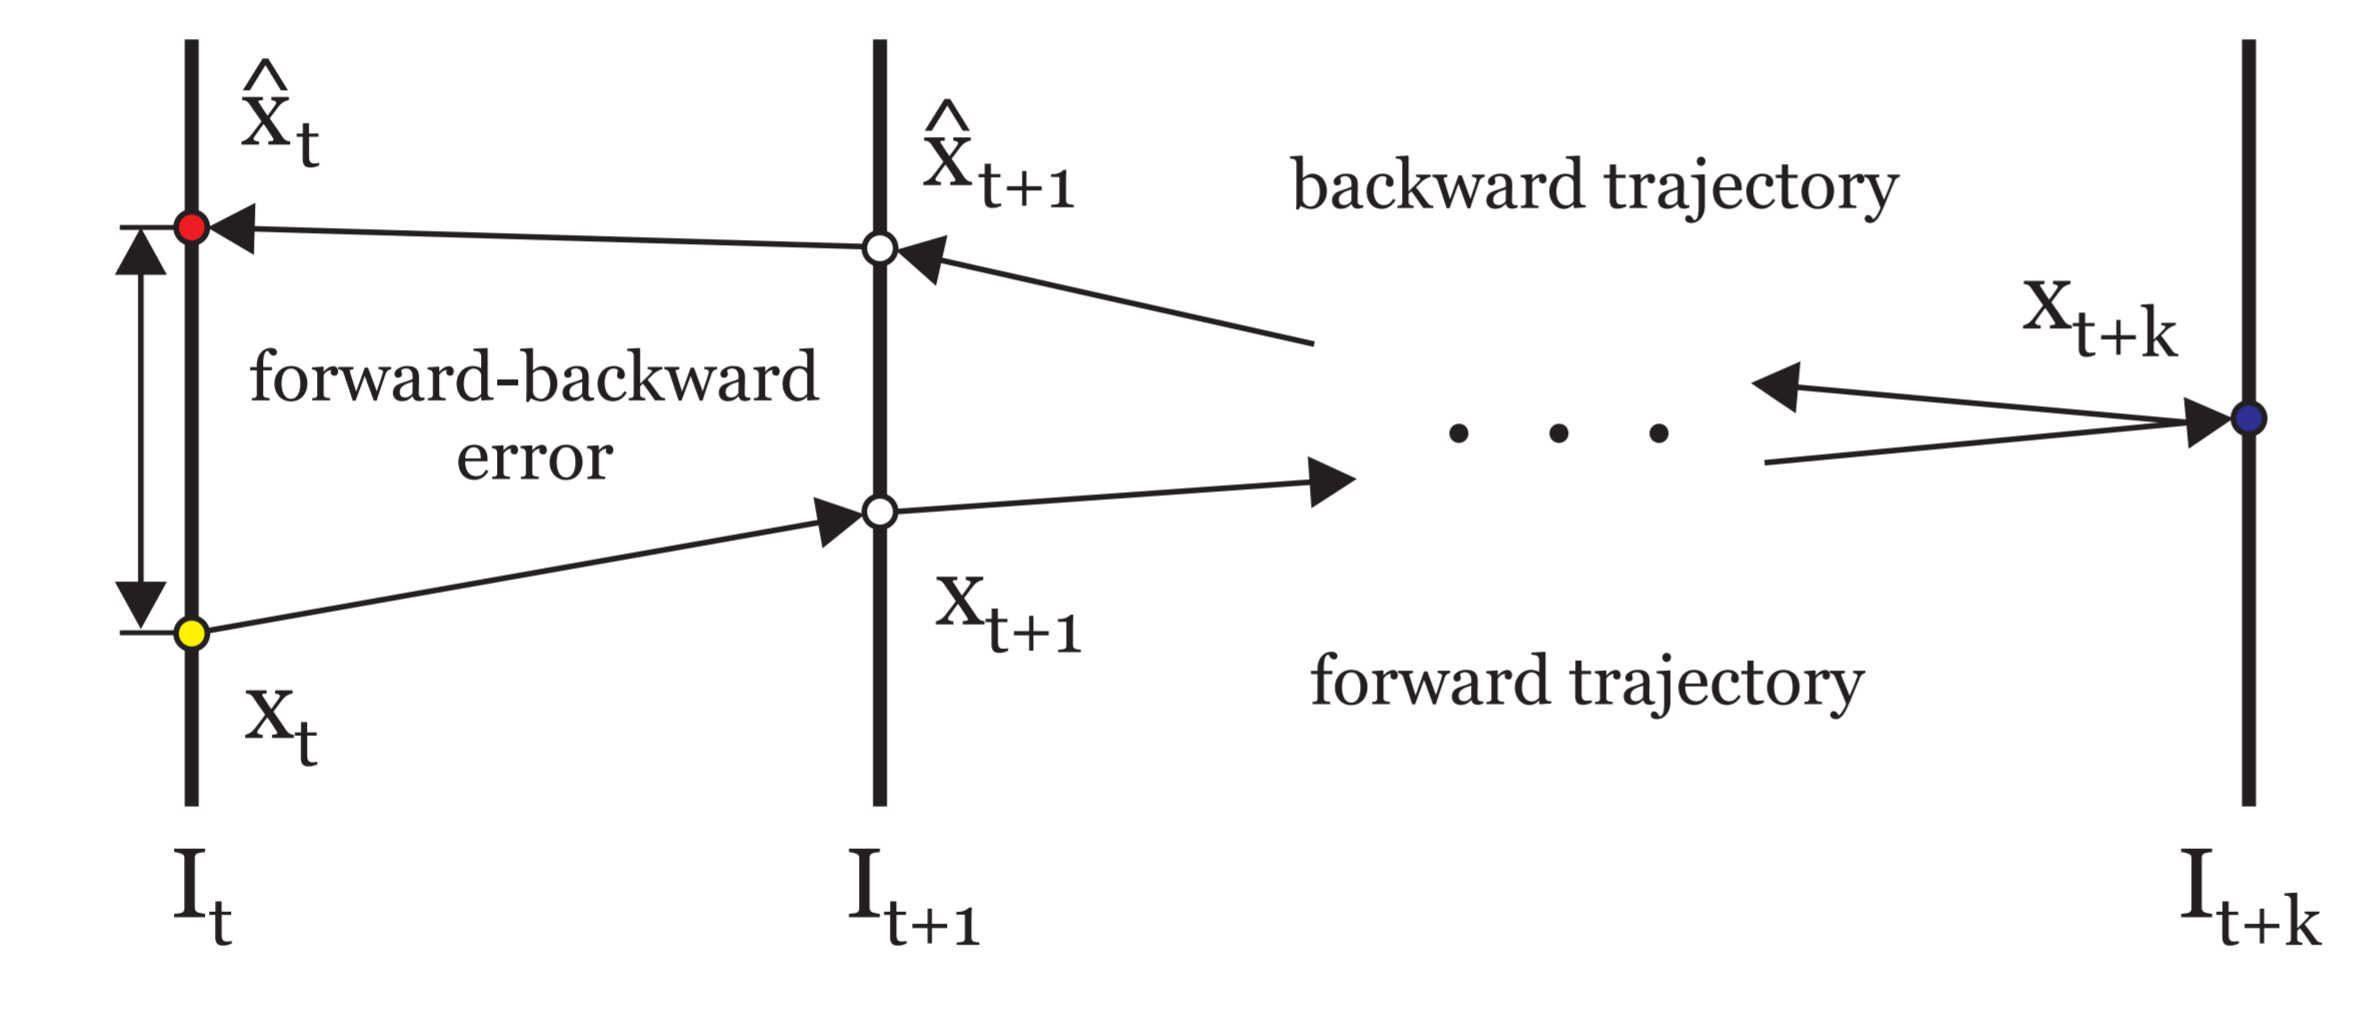
\includegraphics[width=7cm]{tracker/forwardBack2.png}}\\
\caption{Illustration forward backward error.}
\label{experiTrack5}
\end{figure}


We also implemented the forward method. We replaced for the tracking module in the algorithm. In the table \ref{tableResultsTrack} we observe the result of the forward and the forward-backward methods. Both have the same MOTA but the forward-backward methods takes around 10 $\%$ more time. Both have got the same accurcy but the forward-backward method is slower. For these reasons we decided to not use the forward-backward method and use the forward method in our solution.

\begin{table}[H]
\centering

\resizebox{\textwidth}{!}{\begin{tabular}{l|llll|lll|ll|l}
              &  \textbf{GT} & \textbf{MT} & \textbf{PT} & \textbf{ML} & \textbf{FP} & \textbf{FN} & \textbf{IDs} &  \textbf{MOTA} & \textbf{MOTP} & \textbf{FPS} \\
\textit{Forward}   & 517         & 3           & 127         & 387         & 18896       & 78999       & 618             & 10.8          & 68.1                & 15.85        \\
\textit{Forward-Backward}  & 517         & 11          & 181         & 325         & 19951       & 78940       & 827                  & 9.7           & 67.3                  & 9.0          \\
  
\end{tabular}}
\caption{Comparison tracking modules.}
\label{tableResultsTrack}
\end{table}

\subsection{Tracking analysis}

In this part we realize a qualitative analysis of the tracking module. The main disadvantage of the feature-based tracking is the dependence on the quality of the features, this method needs blobs with high texture to accomplish a good tracking. Thus, a sequence of low resolution there are less points with these characteristics. Also, we have problems with people who wear low texture clothes or are away from the camera, as we can observe in figure \ref{Fails1}.


\begin{figure}[H]
		
\centering

\subfigure[High texture person.]{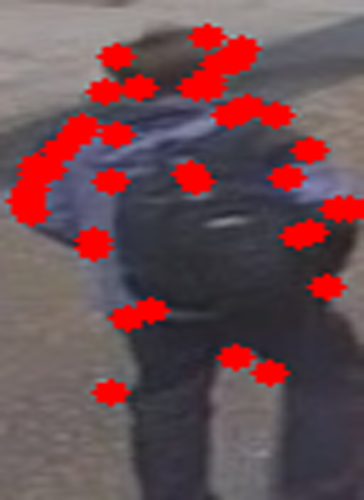
\includegraphics[width=5cm]{changeCamera/tomeuTetx.png}}
\subfigure[Low texture person.]{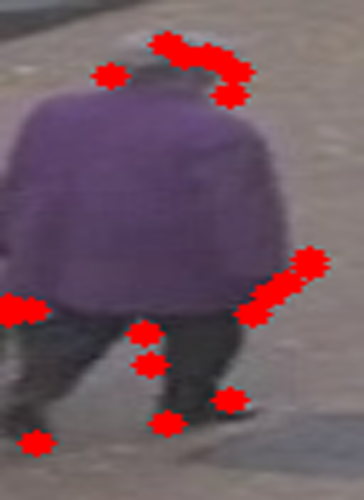
\includegraphics[width=5cm]{changeCamera/donaTetx.png}}
\subfigure[Far away person.]{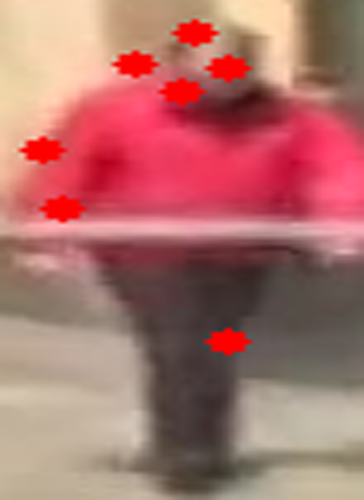
\includegraphics[width=5cm]{changeCamera/foto004.png}}
\caption{Differences texture examples.}
\label{Fails1}
\end{figure}


Although a low frame rate could penalize the matching capabilities between frames, the pyramidal implementation of the Lucas-Kanade method solve it. In the figure \ref{fails2} we show the matching procedure of a blob belonging to a low frame rate sequence, and its result is correct.


\begin{figure}[H]
\centering         
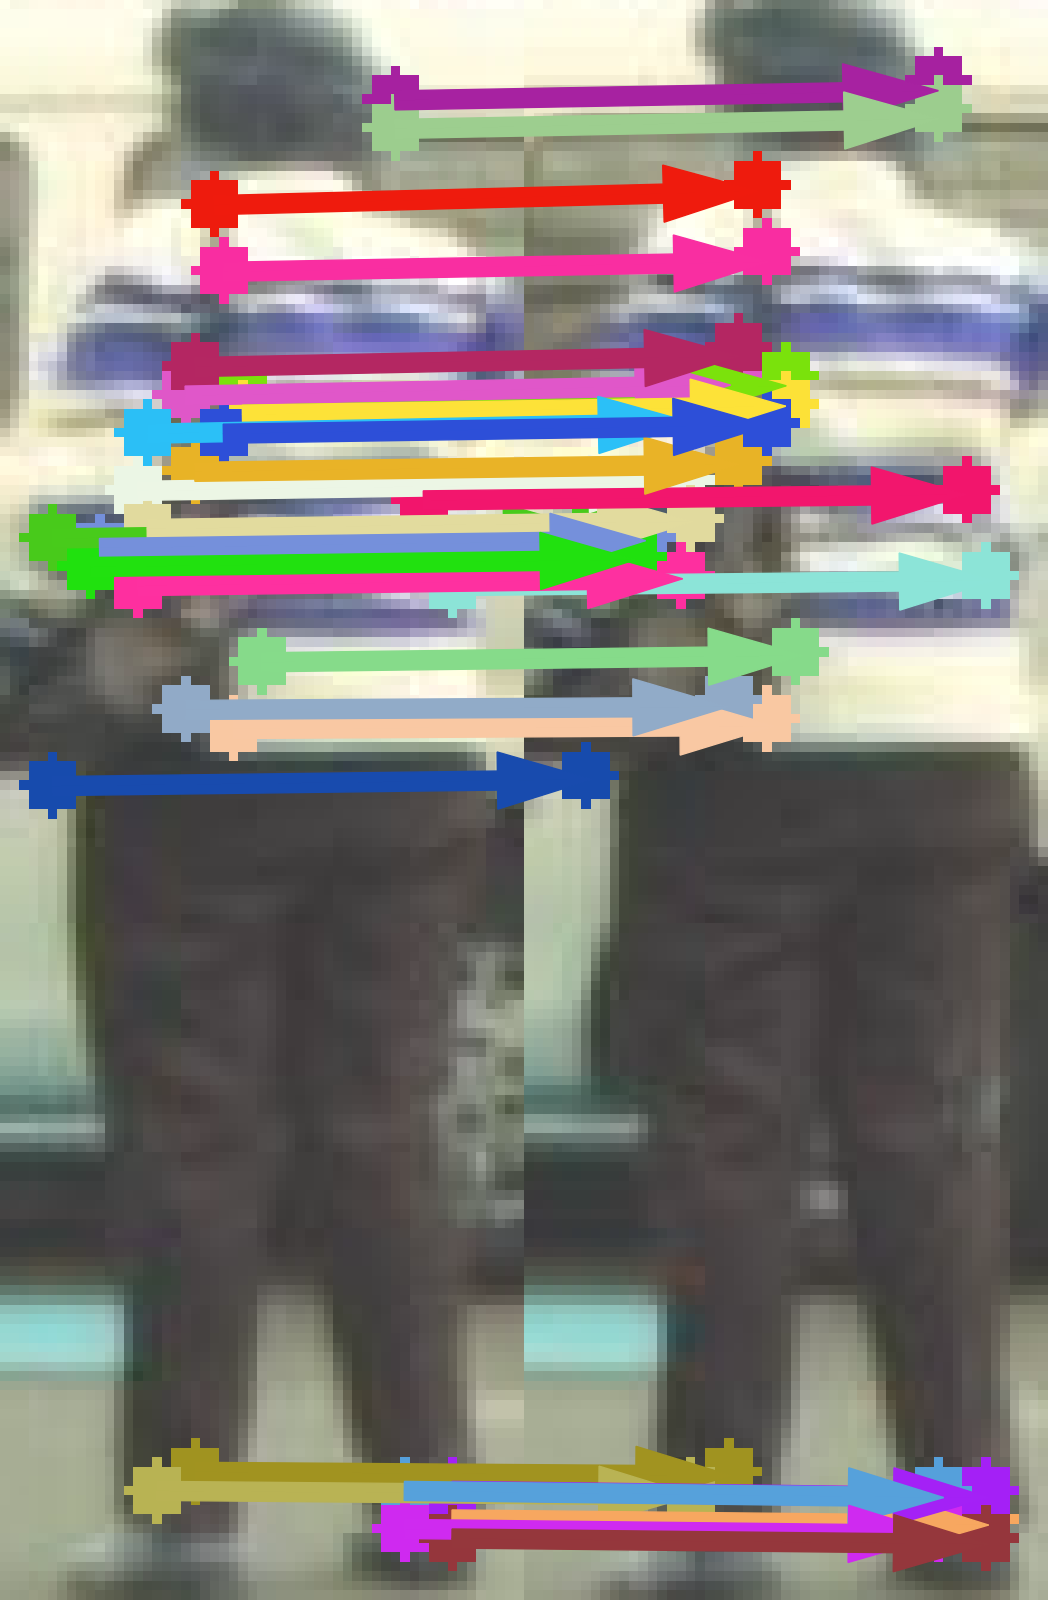
\includegraphics[width=6cm]{lucasKanade/matchinBo.png}
\caption{Blob matching low frame rate sequence.} \label{fails2}
\end{figure}



\section{Data Association experiments}\label{exper:entrenar}



With this module we want to solve the person reidentification problem generate in the feature-based tracking module. This module wants to check whether some blobs detections are new in the scene or have been seen previously. Thus, these architectures takes two blobs images as input and compute the probability to belong to the same identity. We tested how perform this task five architectures based on neural networks and we chose the best to incorporate on our tracking algorithm: 



\begin{itemize}


\item \textbf{Siamese network: Cost function}, this is based on the idea of deep learning as feature extractor and top layers as classifier. Two branches that share parameters process the images and classify it.

\item \textbf{Siamese network: In-network}, this is a mix of the previous models, where the information of the convolutional layers merges at some point before the classifier.

\item \textbf{Siamese network: Joint data input}, according to the literature this architecture gives the best results compared with the other topologies. The input of the network is a concatenation of the two images and the network processes them together.


\item \textbf{Feature extractor with cosine distance}, we used well-known architectures for image classification to extract features from the images and then compare those features with the cosine distance.

\item \textbf{Famous network fine-tuned}, we extract features for each image with a well-known architecture and merge them  with a fully connected layer.

\end{itemize}

We can observe these architectures in the figure \ref{siameseData1}.

\begin{figure}[H]
		
\centering

\subfigure[Cost function.]{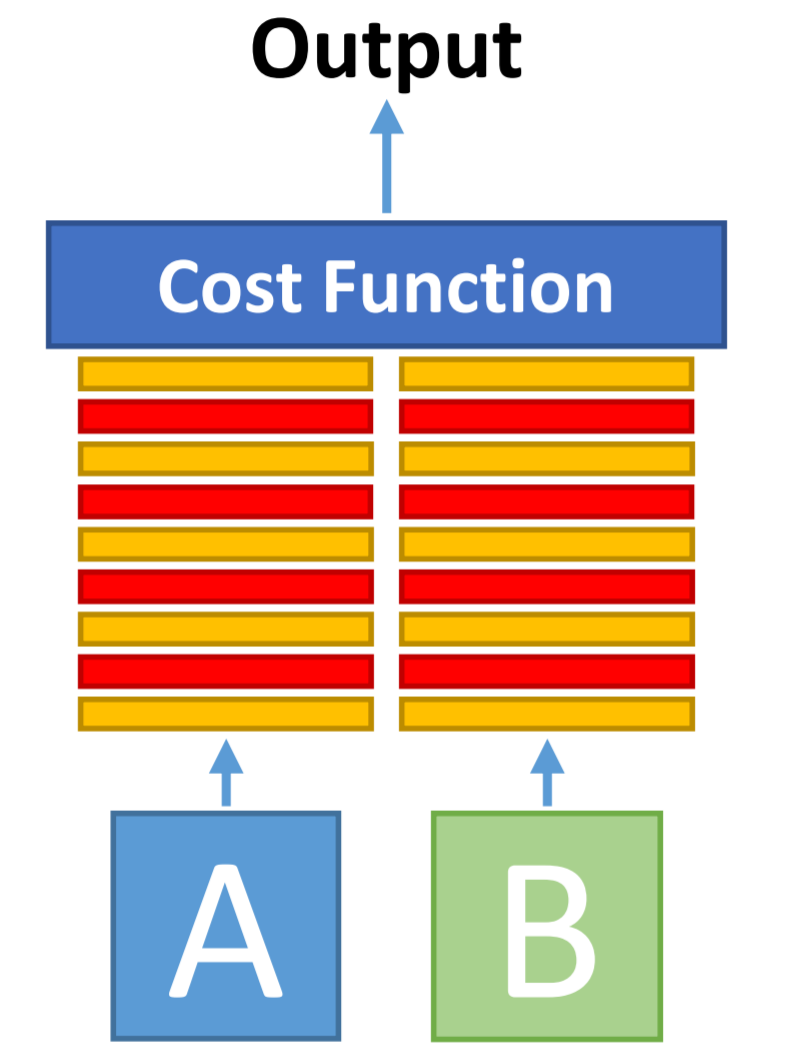
\includegraphics[width=2.7cm]{siamese/retall1.png}}
\subfigure[In-network.]{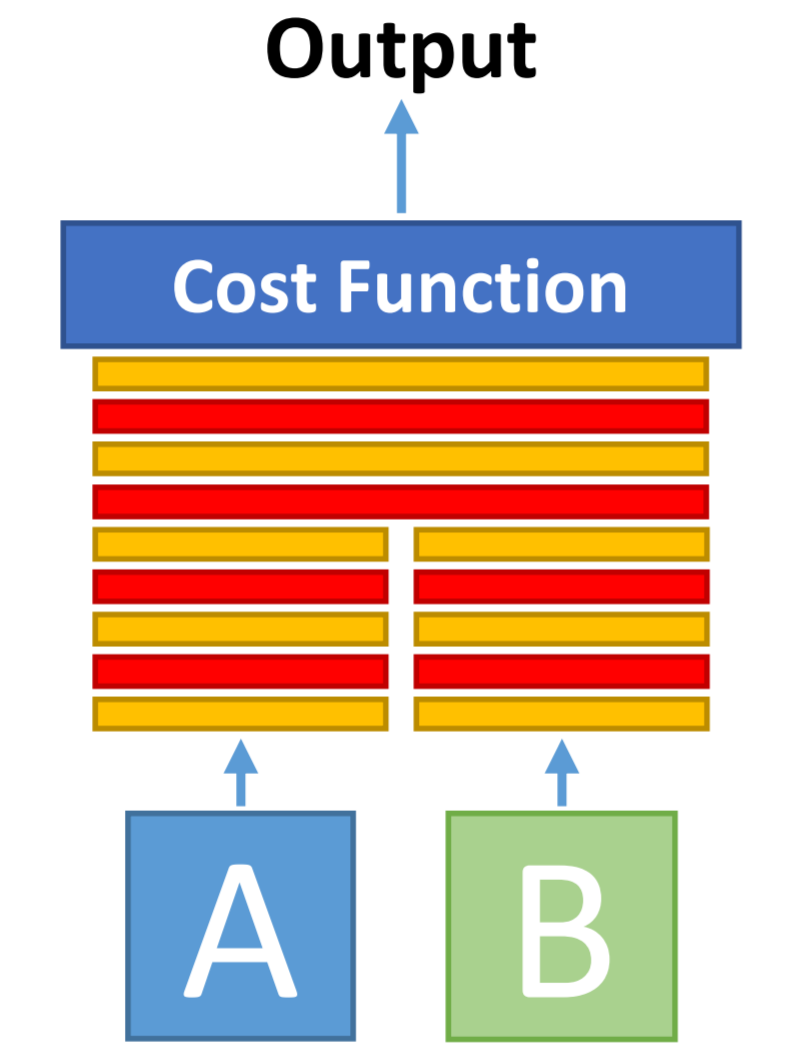
\includegraphics[width=2.7cm]{siamese/retall2.png}}
\subfigure[Joint data input.]{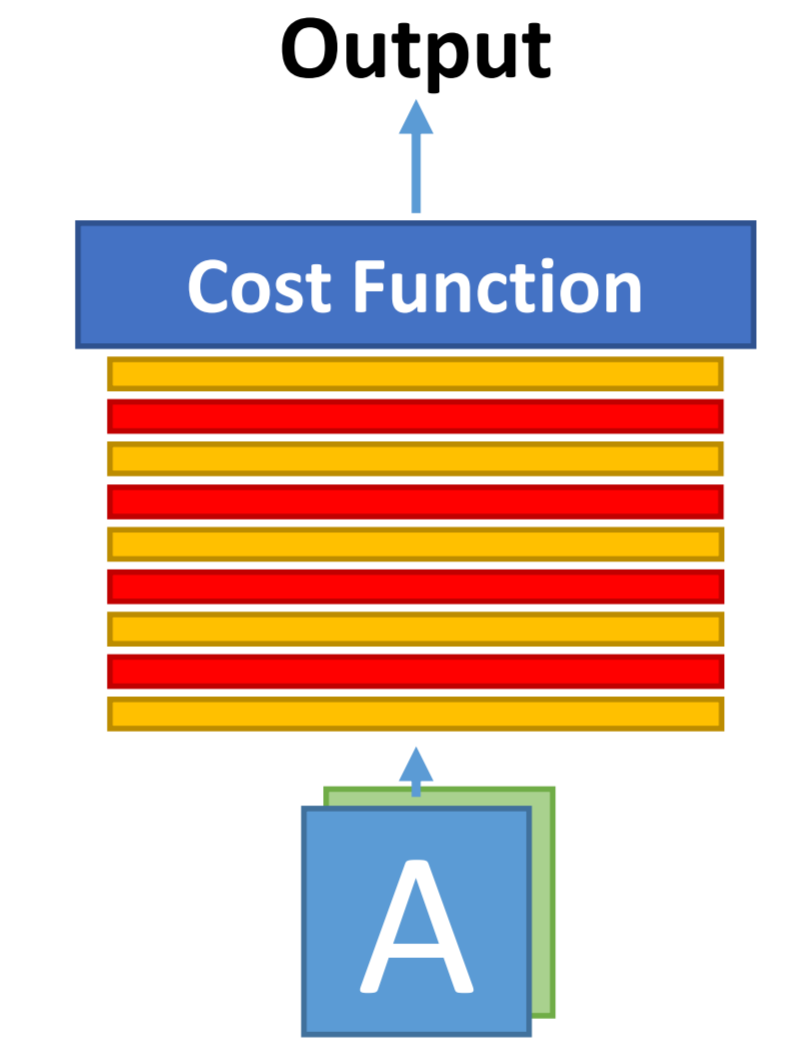
\includegraphics[width=2.7cm]{siamese/retall3.png}}
\subfigure[Features with cosine distance.]{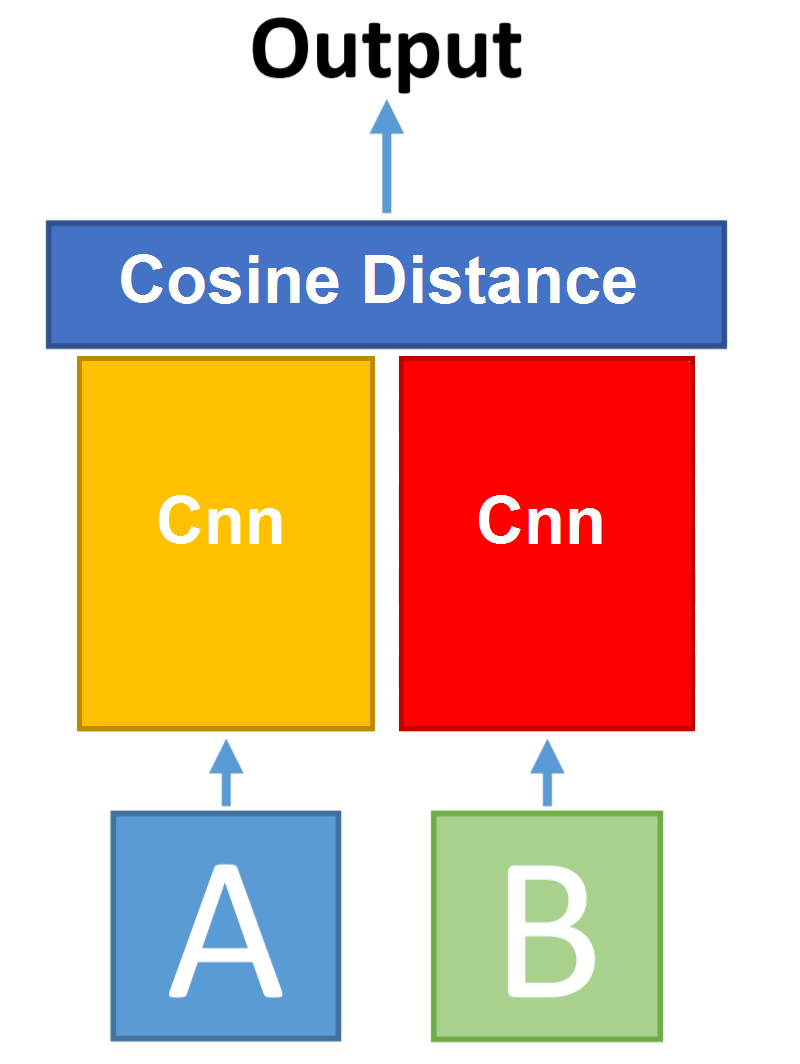
\includegraphics[width=2.7cm]{siamese/cosineDistance.png}}
\subfigure[Cnn fine-tuned.]{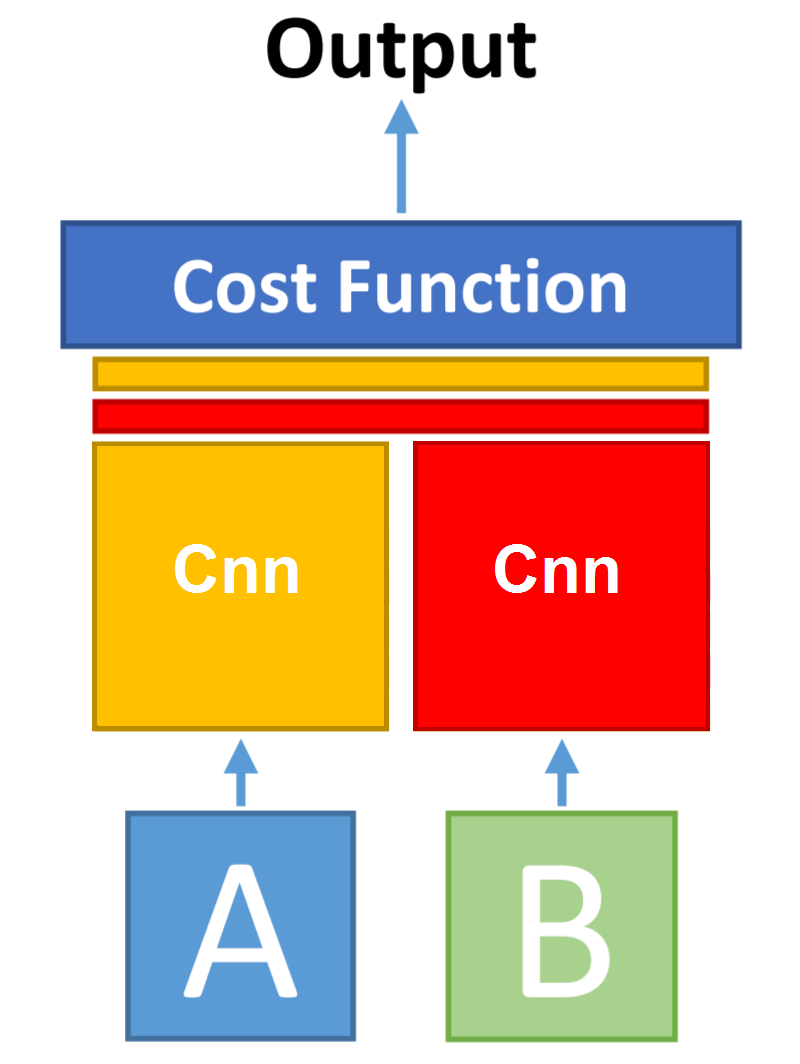
\includegraphics[width=2.7cm]{siamese/retall2cnnMAss.png}}\\


\caption{Siamese CNN topologies.}
\label{siameseData1}
\end{figure}


The main characteristics of the trained networks are the following:

\begin{itemize}

\item \textbf{Loss}, we used the binary cross entropy as a loss. We tried with the contrastive divergence but it did not converge.

\item \textbf{Optimizer}, as optimizer we used Adam, even though it has a mechanism to decrease the learning rate. We added an exponential decay to speed up the convergence

\item \textbf{Activation}, we used ReLu. Currently, there are other activations functions, but ReLu has been established as the reference.

\item \textbf{Initialization}, to initialize the weights we used the He. initialization method \cite{hemethod}. In addition we initialized the biases with the value of $0.1$, in this way we avoid the dead neurons in the firsts iterations.

\item \textbf{Batch normalization}, we tested batch normalization, but it adds to much computation time and so we discarded it.

\item \textbf{Regularization}, we used Dropout in the fully connected layer to avoid overfitting.

\item \textbf{Preprocessing}, as preprocessing techniques we centre the data.  We subtract the mean per channel calculated over all images. Also, we normalized the data between the range 0 and 1.

\item \textbf{Final layers}, historically, in the junction between the convolutional layers and the fully connected layer, a flatten mechanism has been used, but it increases dramatically the number of neurons in the fully connected layer, and it shows problems to converge. From the publication of InceptionV3 \cite{inception33}, the authors used a global average pooling layer, it generates the spatial average of each channel of the tensor. With this layer we achieve a reduction on the number of neurons in the fully connected layers and the nerwork converges quickly. Also we used the spatial pyramid pooling layers, they consist of a multiresolution max pooling. We can observe those differences in \ref{siameseData2}.

\begin{figure}[H]
		
\centering

\subfigure[Flatten.]{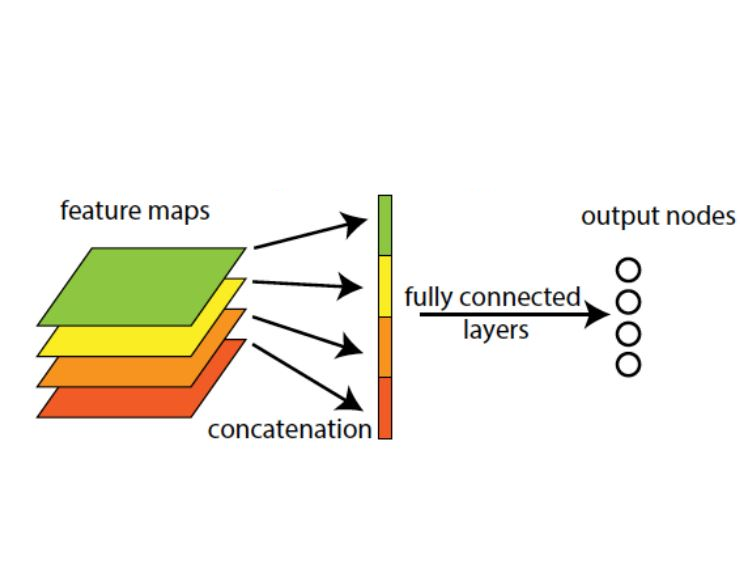
\includegraphics[width=6.5cm]{siameseDev/flatten2.png}}
\subfigure[Global average pooling.]{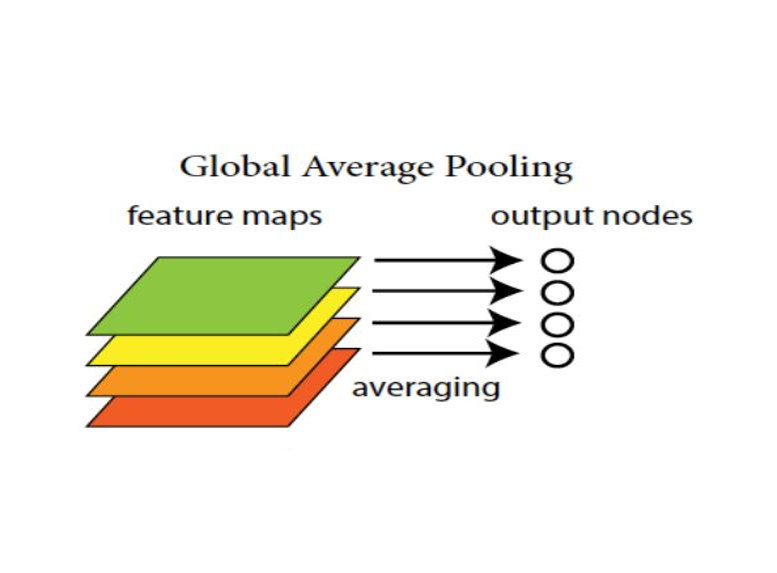
\includegraphics[width=6cm]{siameseDev/global2.png}}
\subfigure[Spatial pyramid pooling.]{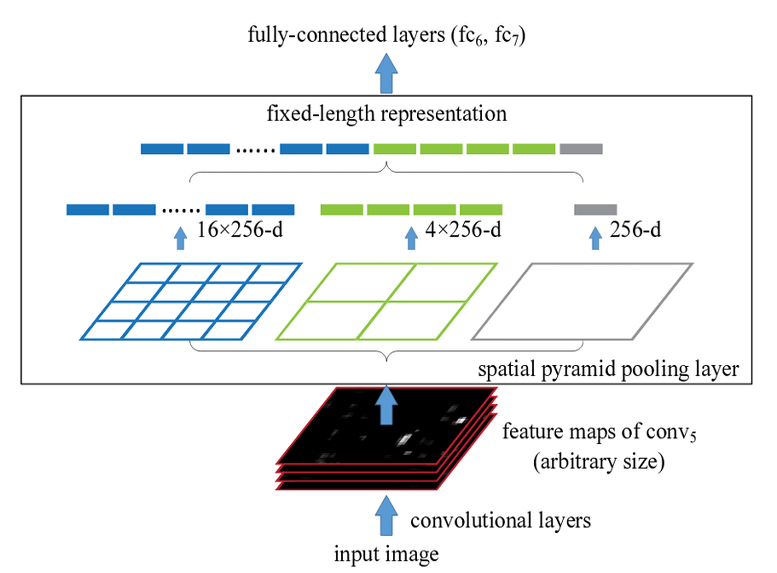
\includegraphics[width=8cm]{siameseDev/spp2.png}}\\



\caption{Final layers.}
\label{siameseData2}
\end{figure}


\item \textbf{Output}, We did not use softmax as output, we only used one neuron with sigmoid activation, in this way the output is constrained between $0$ and $1$.



\end{itemize}


%We developed our models in a VGG way, stacking  several convolutional layers and finishing the network with a fully connected layer. We started with a few convolutional layers and added more till we reached an overfitting condition. This condition is considered true when adding more layers the score on the test set declines. We started with $3$ and we end up with $7$ convolutional layers as best performance.

We developed our models in a VGG way, stacking  several convolutional layers and finishing the network with a fully connected layer. We started with a few convolutional layers and added more till the score on the test set does not improve. We started with $3$ and we end up with $6$ convolutional layers as best performance.

For the dataset, there is not a prominent dataset in the field, so at the beginning we decided to use the MOT16 as dataset and adapt it to our needs. In order to do so, we extracted the detections with their identities, and then for each identity we selected all possible random pairs as positive examples. For the negative set we selected several random identities. The negative dataset is much bigger than the positive dataset, so we limited it to have a balanced dataset. The problem with the MOT16 dataset, is that the ground truth was built with the detections of a classifier and there is not a human intervention, resulting in a messy ground truth. We inspected the dataset and around the $70 \%$ of the dataset was wrong, there are a lot of occlusion in detections resulting in wrong pairs, pairs that are not matching with the same identity.

Then, we discarded the MOT16 dataset an used the TownCenter dataset \cite{townCenter} from the University of Oxford instead, which has a manual ground truth. We have got $29824$ positive and negative pairs, then a dataset of $59648$ image pairs. We split the dataset between training and validation set, $80 \%$ and $20 \%$ respectively. For testing we selected a set of identities of the MOT16 dataset. To regularize and enlarge our dataset we applied some data augmentation techniques to our dataset like we observe in figure \ref{msii1}. These transformations consist in: apply a random change of brightness, apply a random crop, apply a vertical flip, apply gaussian blur, appply a random shadow, apply a zoom in, apply a random rotation and translation, apply a zoom out, add gaussian noise, and apply the opposite vignetting. We tried apply all the transformations for each images but then the dataset was too noisy and the network did not converge. So we finally added only one random transformation for each pair, so we double our dataset. We stop their training when its loss do not change in 5 epochs.






\begin{figure}[H]
		
\centering

\subfigure[Original image.]{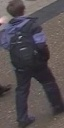
\includegraphics[width=2cm]{dataAugmentation/resizedImage.jpg}}
\subfigure[Random image brightness.]{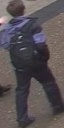
\includegraphics[width=2cm]{dataAugmentation/imageBrightnes.jpg}}
\subfigure[Random crop.]{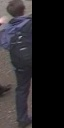
\includegraphics[width=2cm]{dataAugmentation/imageRandomCrop.jpg}}
\subfigure[Vertical flip.]{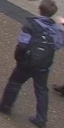
\includegraphics[width=2cm]{dataAugmentation/imageVerticalFlip.jpg}}
\subfigure[Gaussian blur.]{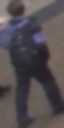
\includegraphics[width=2cm]{dataAugmentation/imageGaussianBlur.jpg}}
\subfigure[Random shadow.]{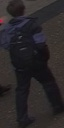
\includegraphics[width=2cm]{dataAugmentation/imageRandomShadow.jpg}}


\subfigure[Zoom in.]{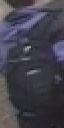
\includegraphics[width=2cm]{dataAugmentation/imageZoomIn.jpg}}
\subfigure[Rotation and translation.]{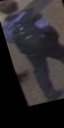
\includegraphics[width=2cm]{dataAugmentation/imageTransormed.jpg}}
\subfigure[Zoom out.]{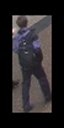
\includegraphics[width=2cm]{dataAugmentation/imageZoomOut.jpg}}
\subfigure[Gaussian noise.]{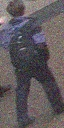
\includegraphics[width=2cm]{dataAugmentation/imageNoiseGaussian.jpg}}
\subfigure[Opposite vignetting.]{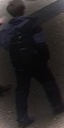
\includegraphics[width=2cm]{dataAugmentation/imageBLURcenter.jpg}}
\caption{Data augmentation.}
\label{msii1}
\end{figure}

%We trained all the models and obtained a graphs like the figure \ref{lossesSiam}, we observe that the network converge, it decreases the loss and increases the accuracy, also we observe that tests plots are a little bit noisy, but we considered that the  regularization techniques are enough. We notice that the joint data input outperforms the other siamese configurations, so we increased the number of layers of that architecture, \textit{conv I}, refers to it, with $I$ the number of layers.


We notice in the first test that the joint data input outperforms the other siamese configurations for the same number of convolutional layers, so we centre in this model. We increased the number of layers of that architecture, \textit{conv I}, refers to this type of model, with $I$ the number of layers. So, we explored conv3, conv4, conv5, conv6, conv7. In the figure \ref{lossesSiam1a} and \ref{lossesSiam2a} we observe the loss and the accuracy on the training and validation sets respectively. We notice that the best models are the conv6 and conv7, they have got a similar results. Despite of the regularization techniques applied to the models are a little bit noisy but it is tolerable ( except conv3, it is too noisy ).

\begin{figure}[H]
		
\centering

\subfigure[Loss.]{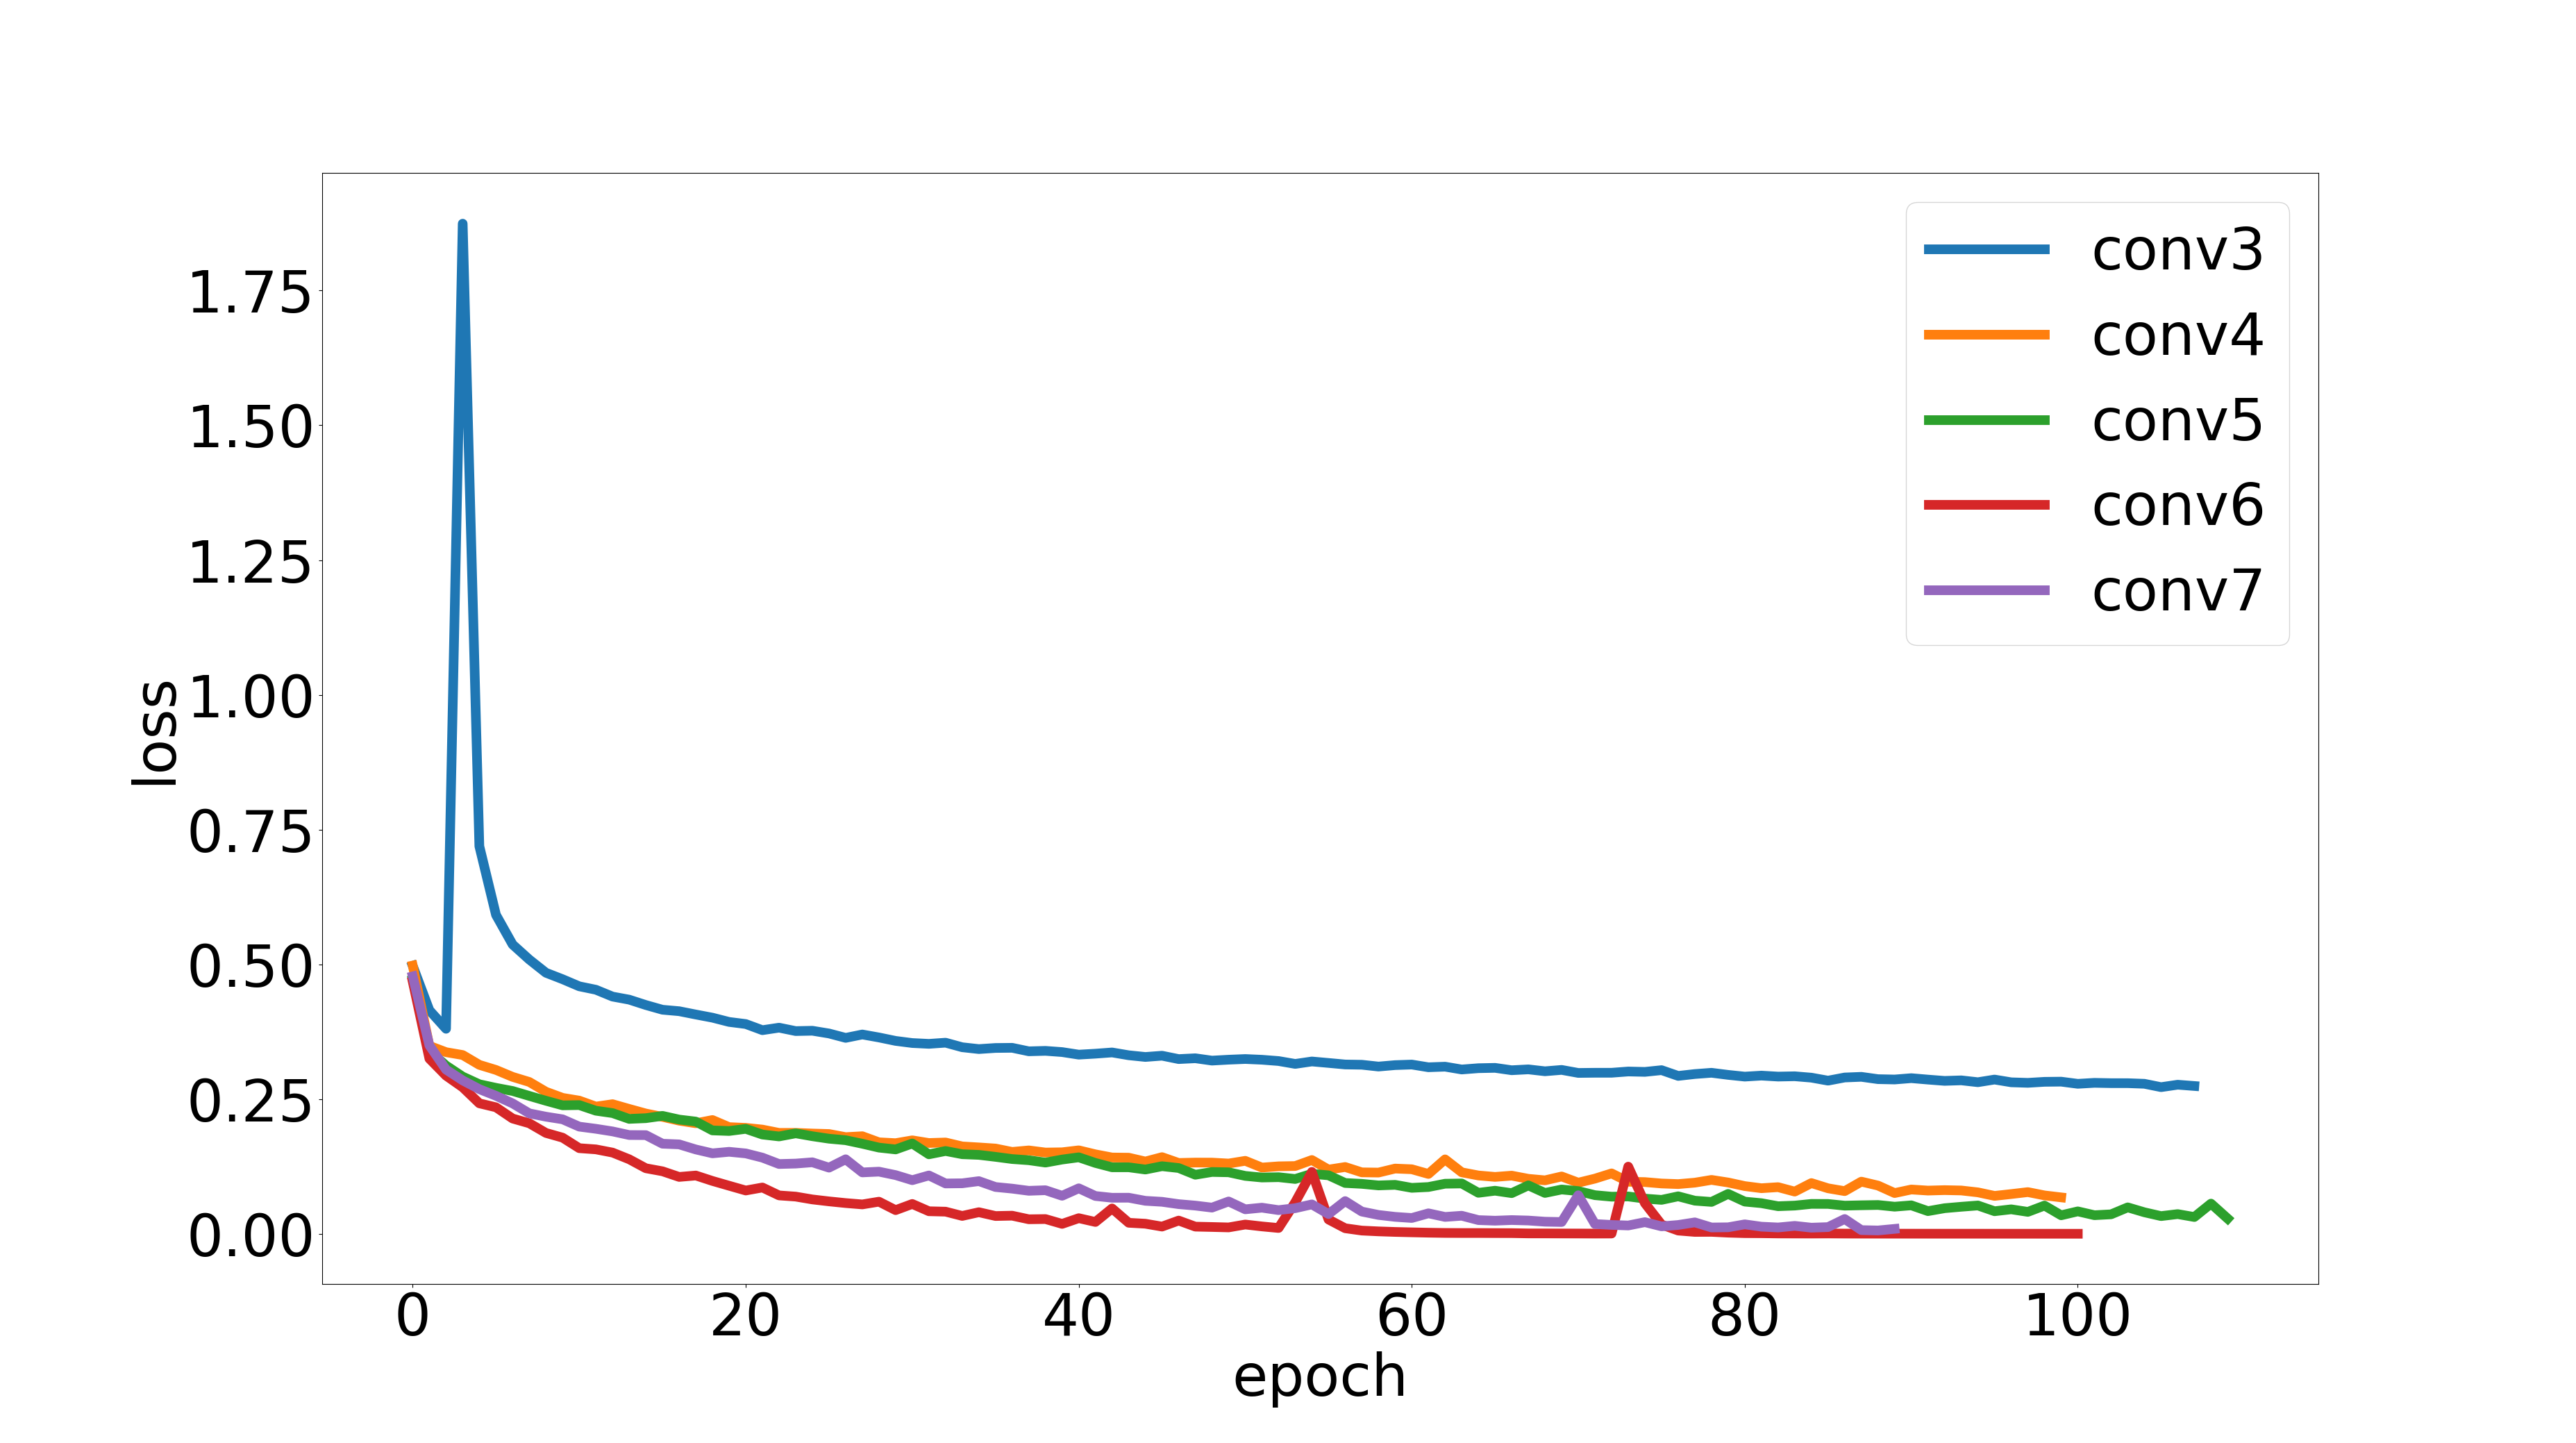
\includegraphics[width=7.5cm]{netss/train-loss.png}}
\subfigure[Accuracy.]{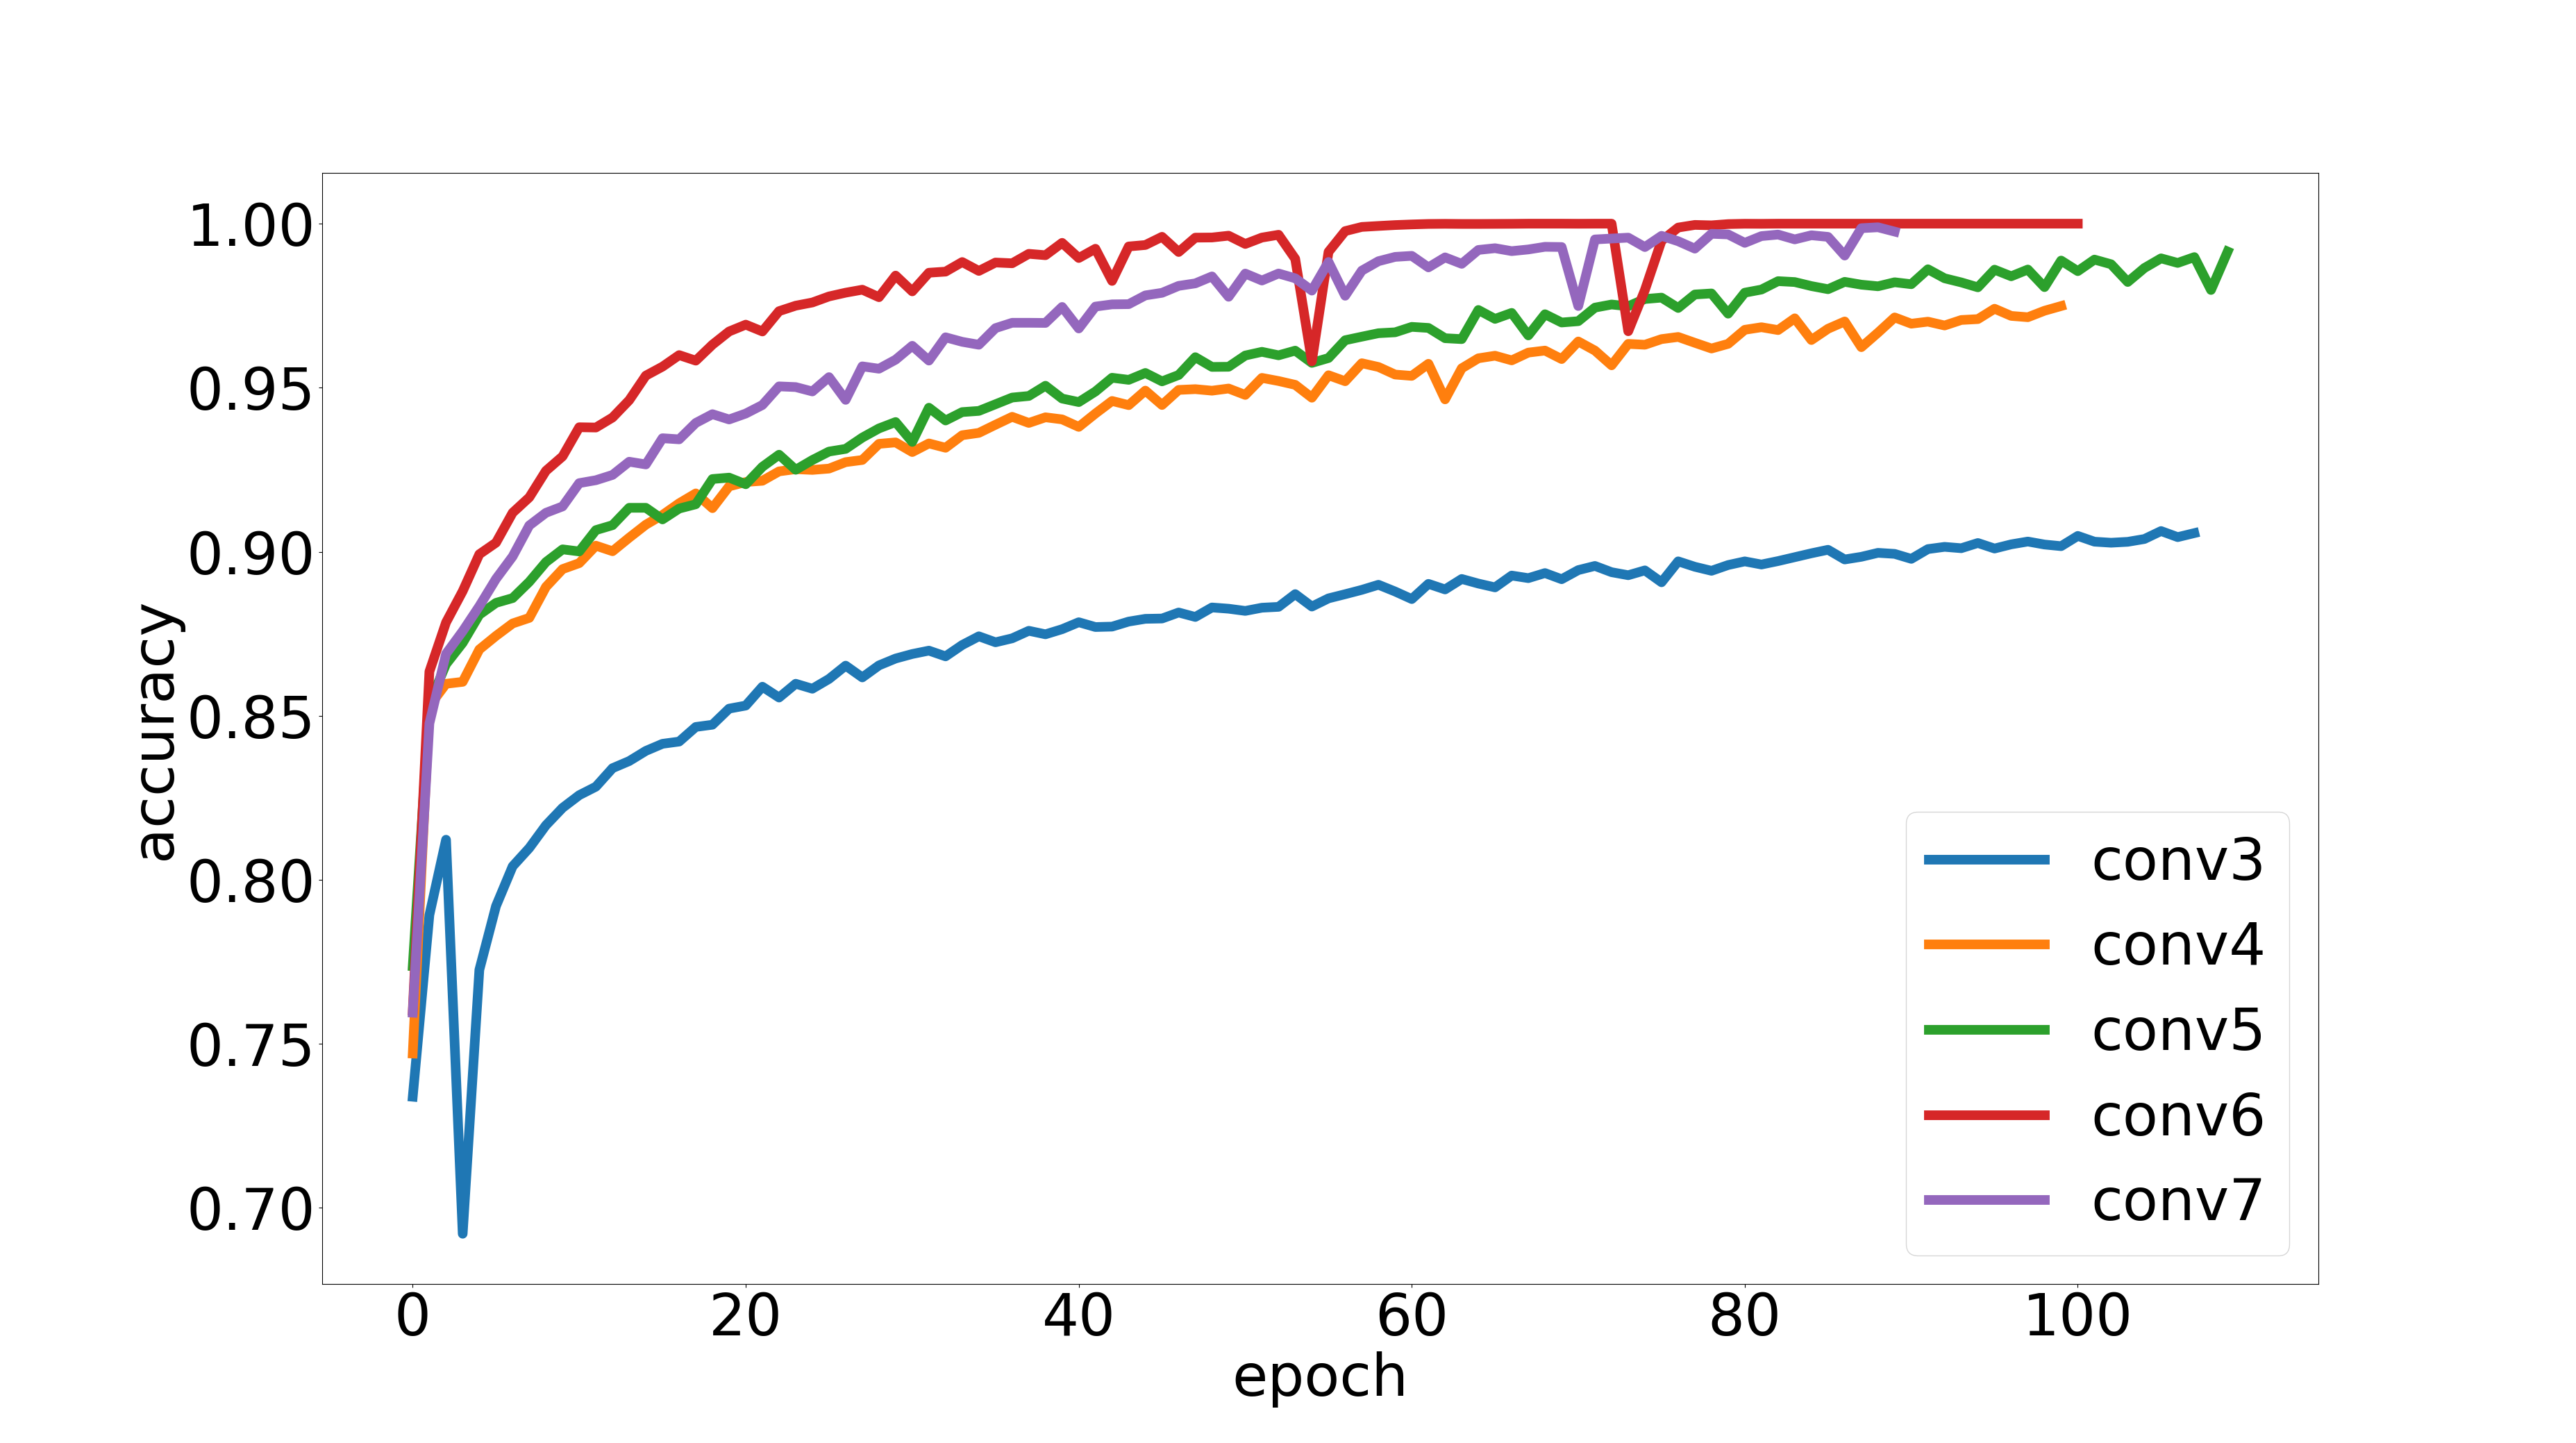
\includegraphics[width=7.5cm]{netss/train-acc.png}}\\

\caption{Results on training set.}
\label{lossesSiam1a}
\end{figure}


\begin{figure}[H]
		
\centering

\subfigure[Loss.]{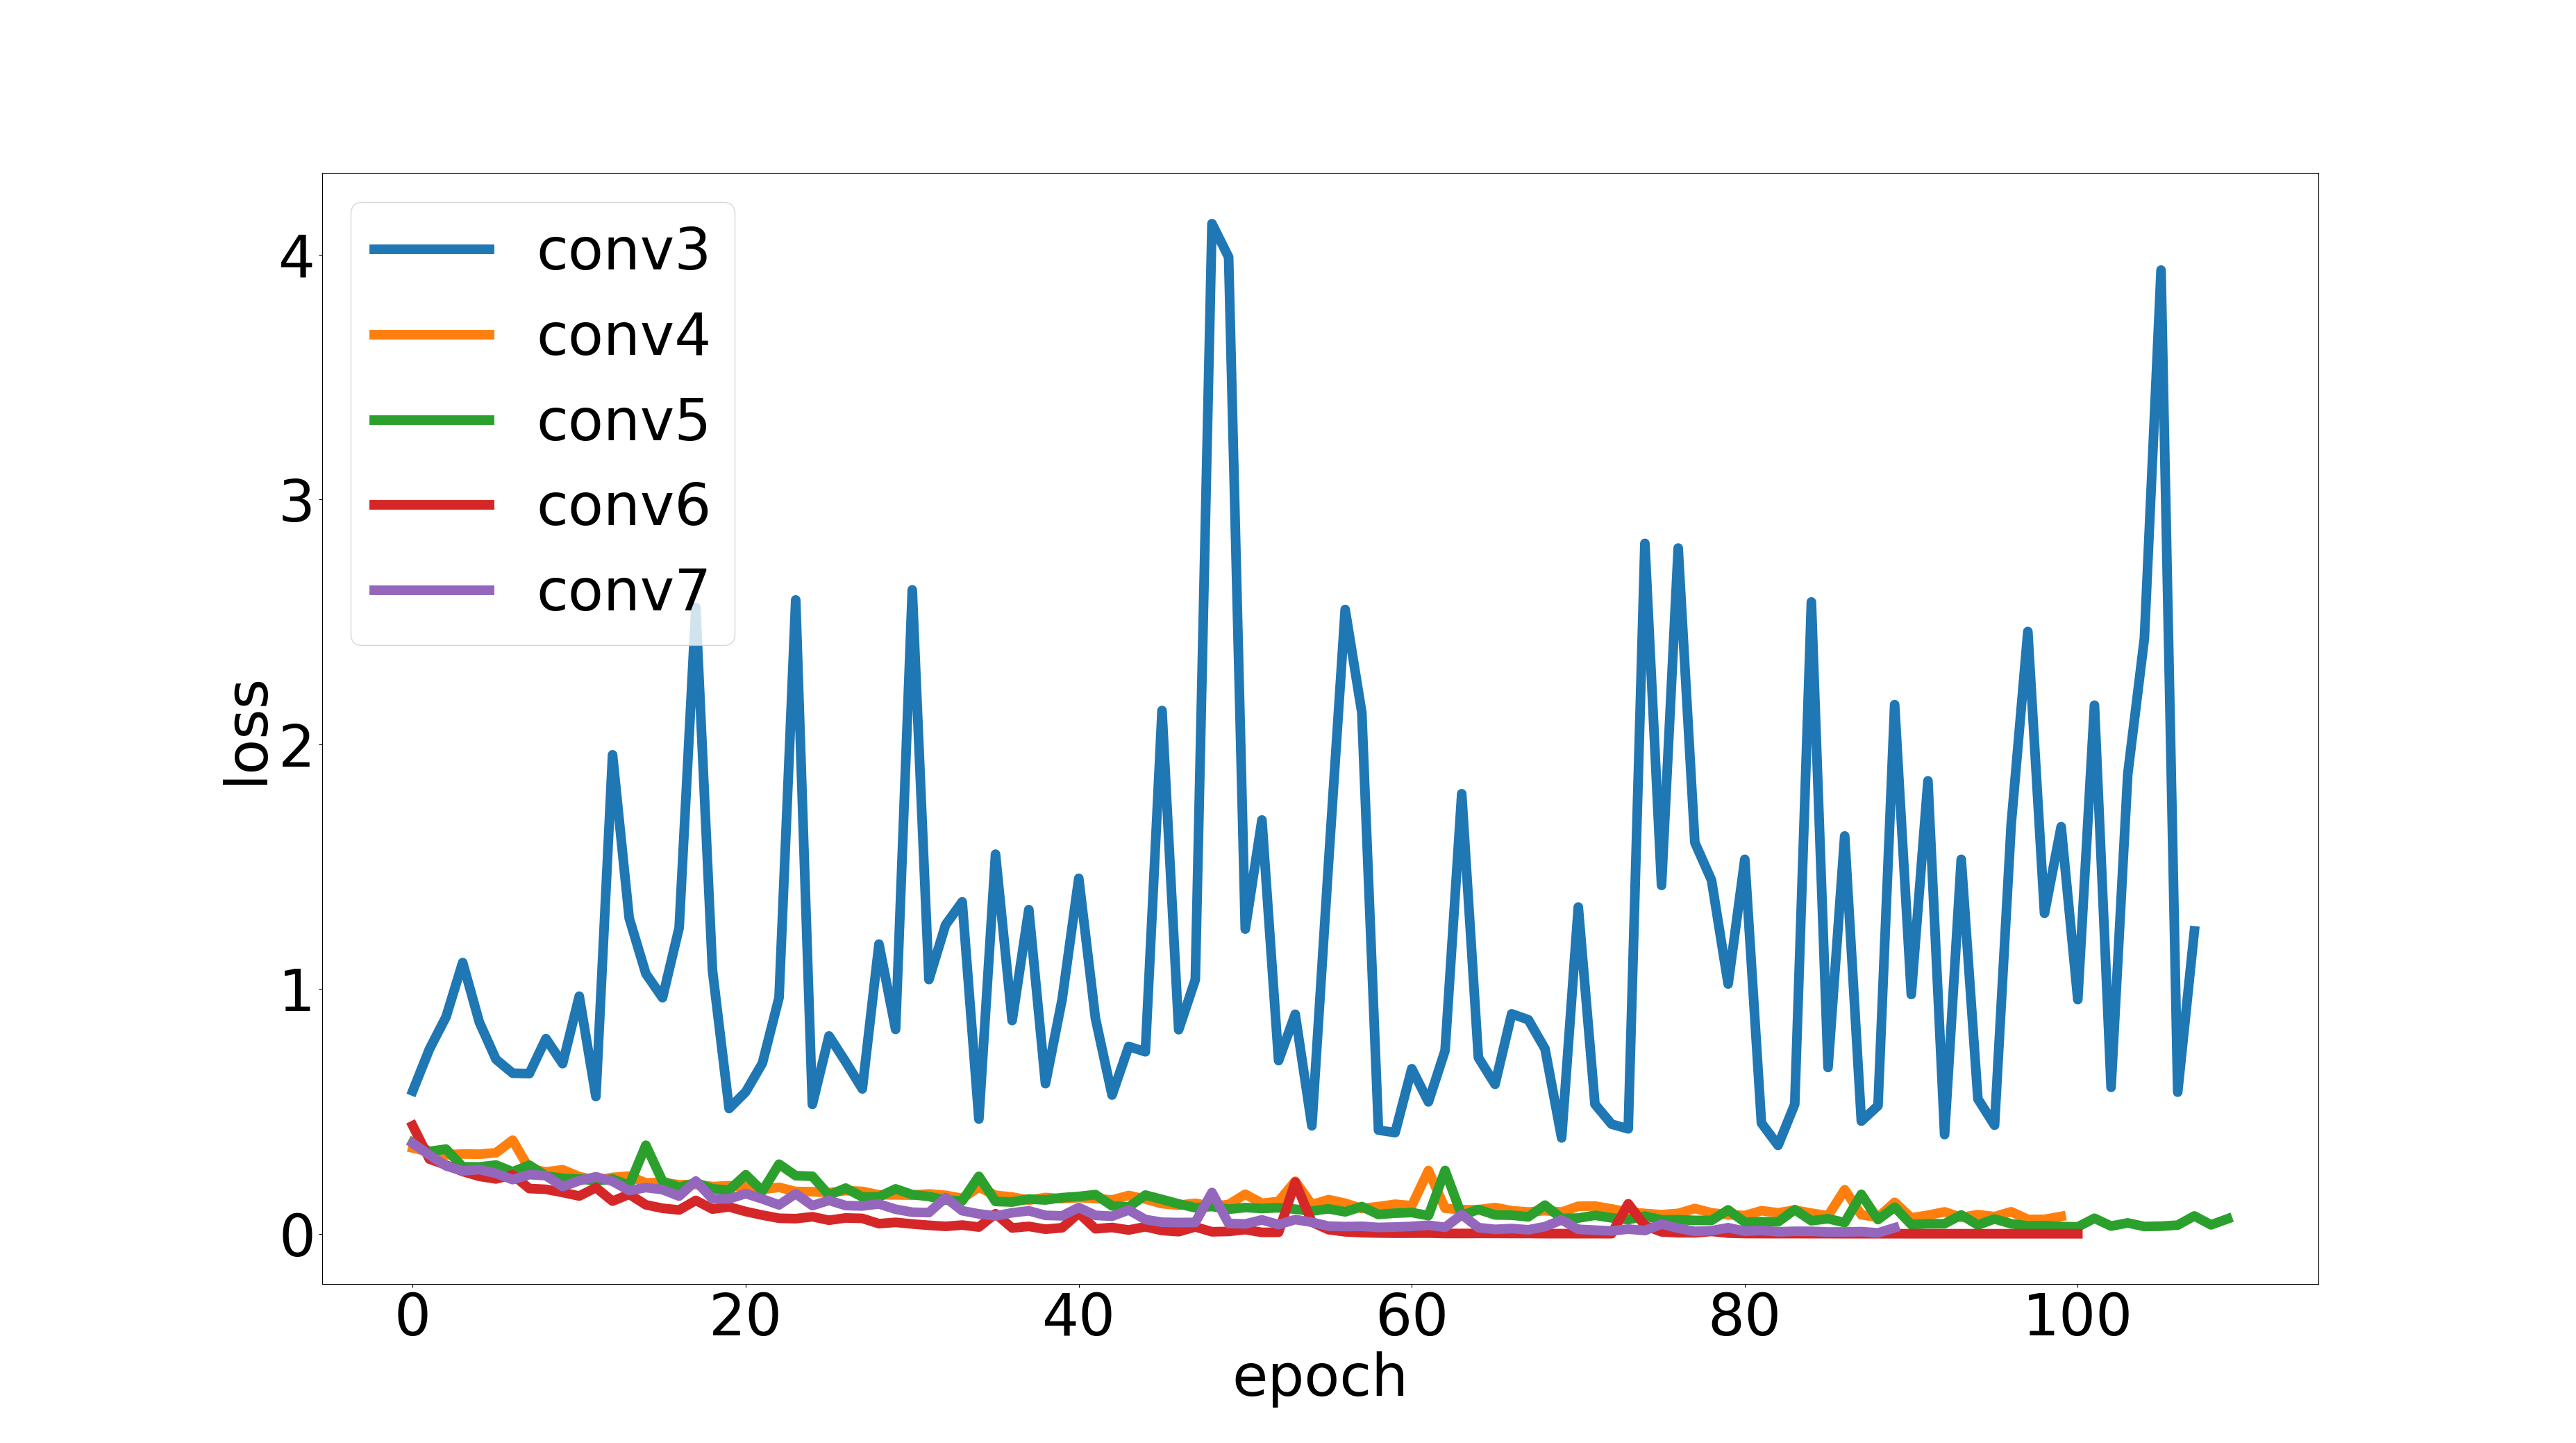
\includegraphics[width=7.5cm]{netss/val-loss.png}}
\subfigure[Accuracy.]{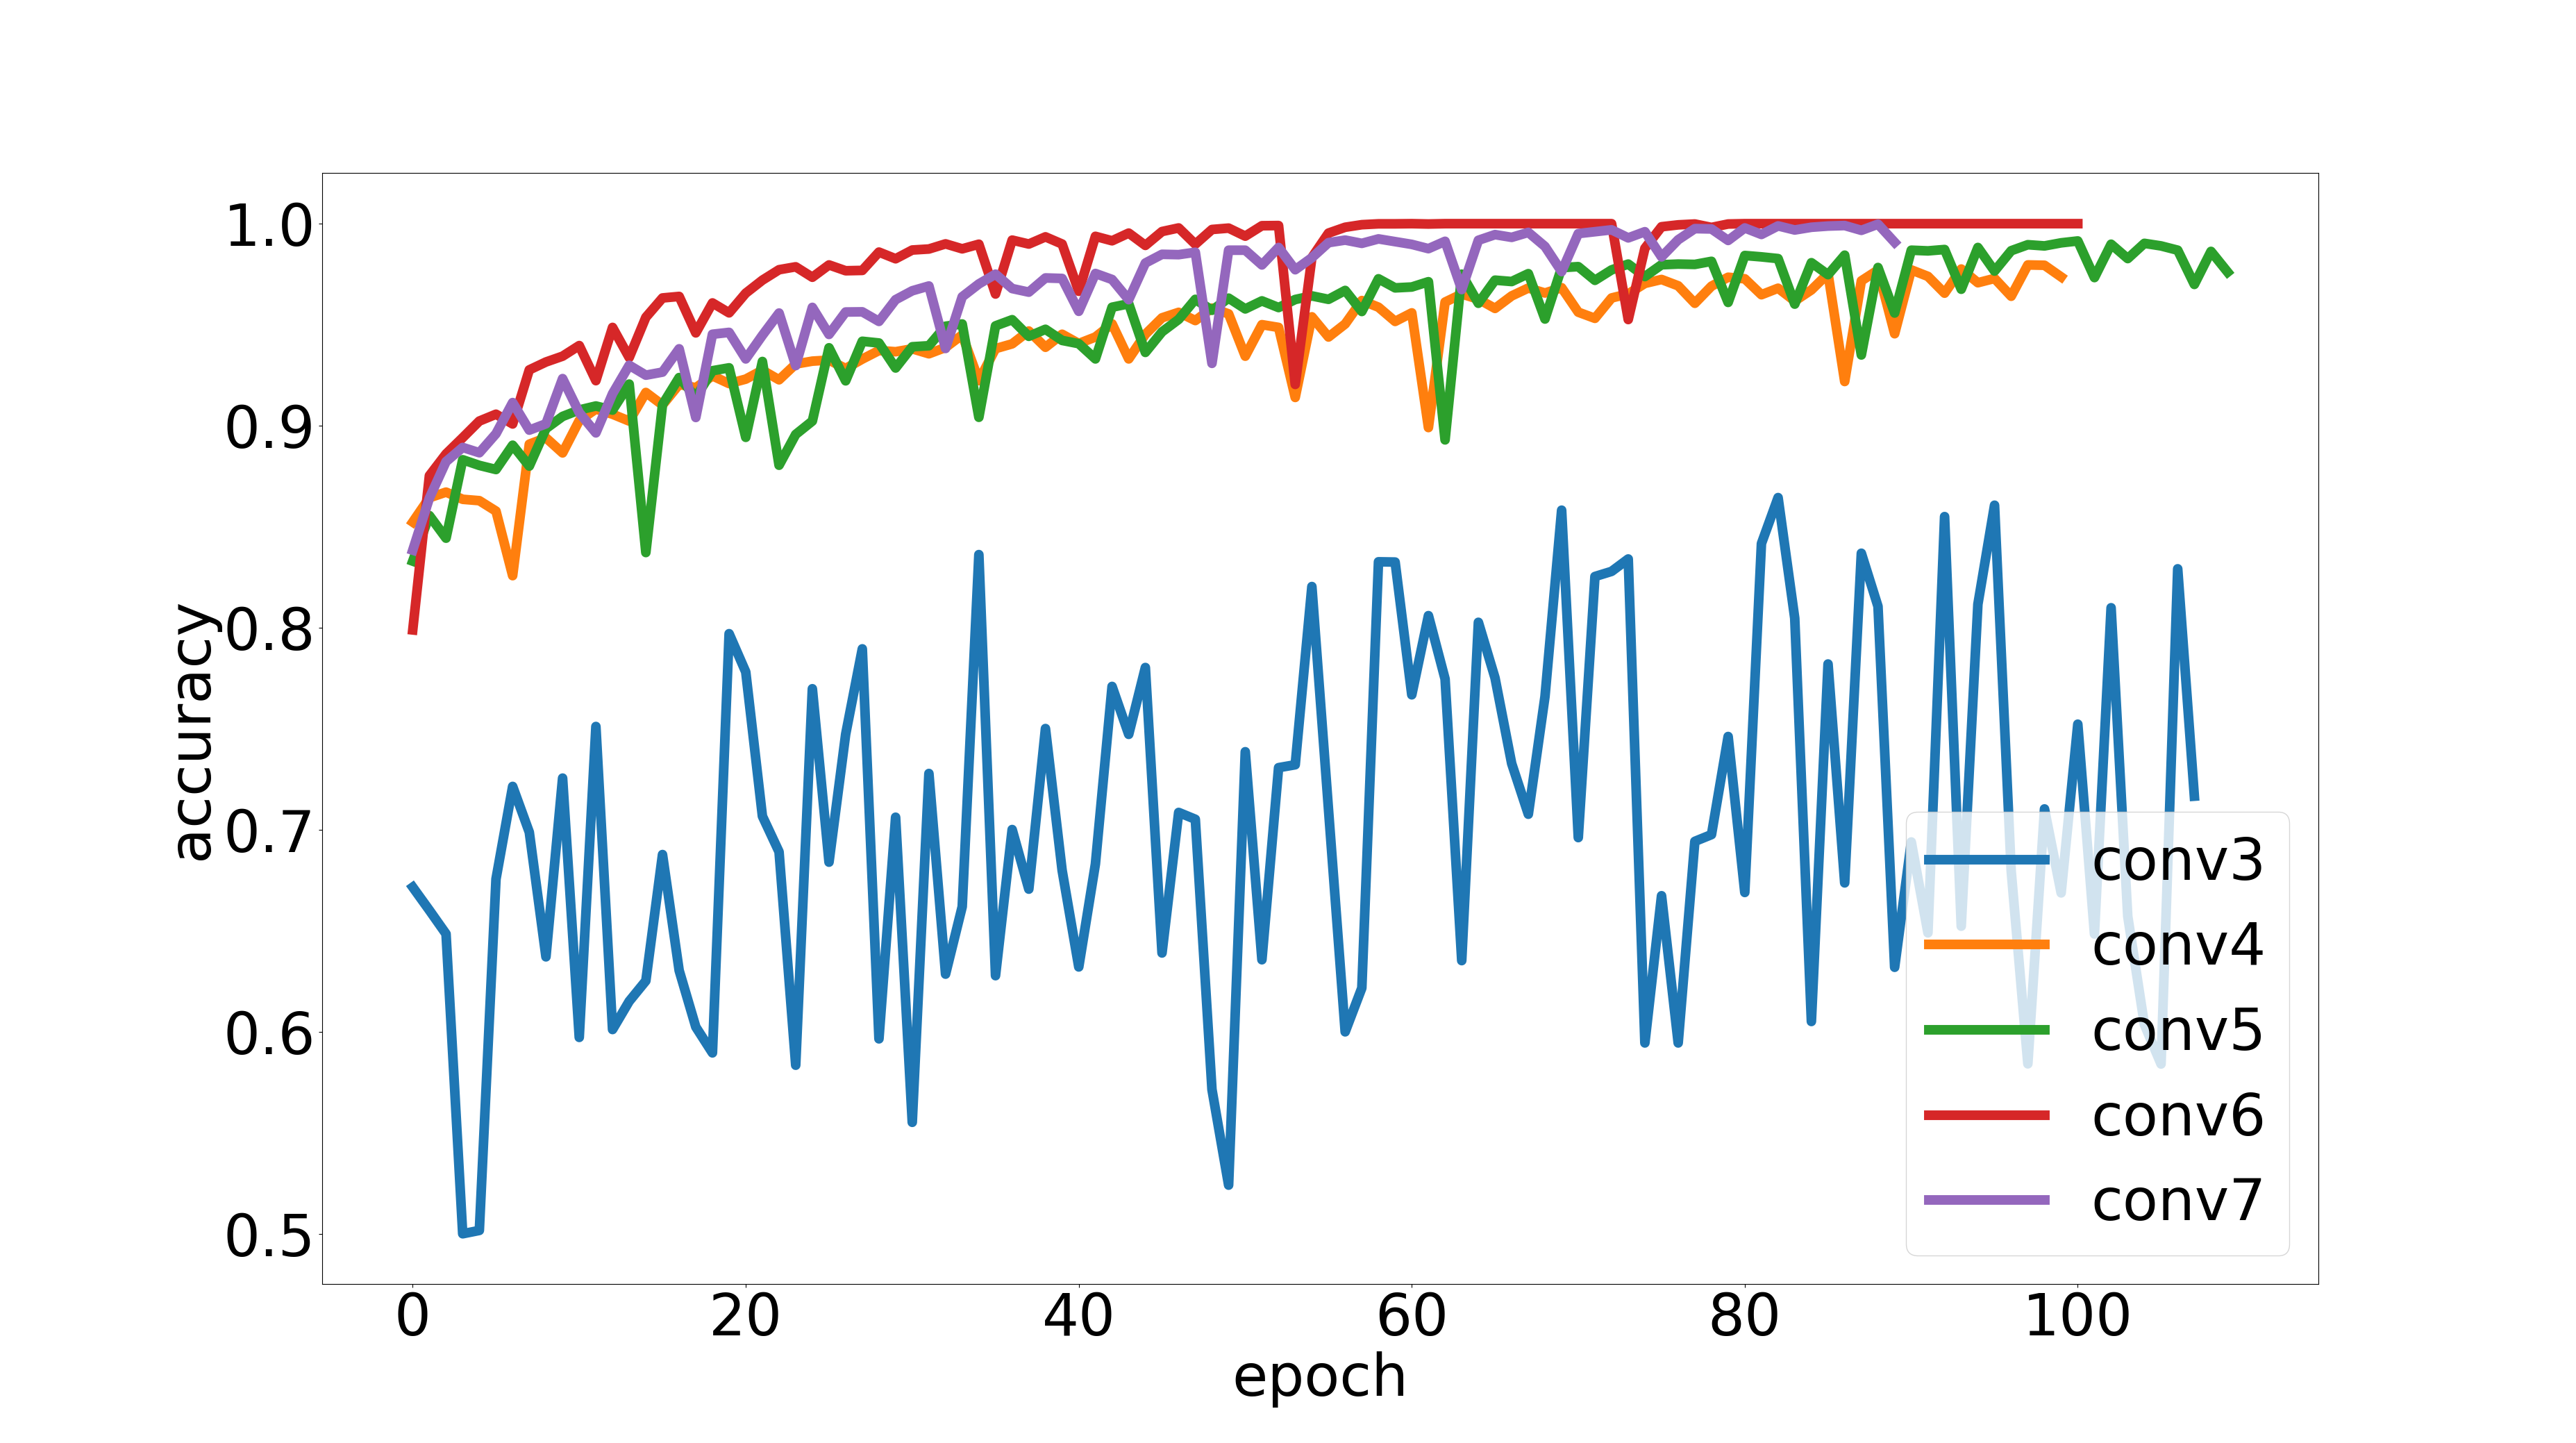
\includegraphics[width=7.5cm]{netss/val-acc.png}}\\

\caption{Results on validation set.}
\label{lossesSiam2a}
\end{figure}



We can observe the comparison using the CMC measure in the figure \ref{lossesSiam2}, we notice that the siamese network with joint data input with less layers performs better than bigger models like Inception. This remarks the idea of training jointly the feature extractor and the classifier and the need of task specific networks. Also, the siamese network with the configuration joint data input outperforms the other siamese networks. Among the siamese joint data input, the performance increases till the $6$ convolutional layer architecture, then performance of the model with $7$ convolutional layers drops.

\begin{figure}[hptb]
\centering         
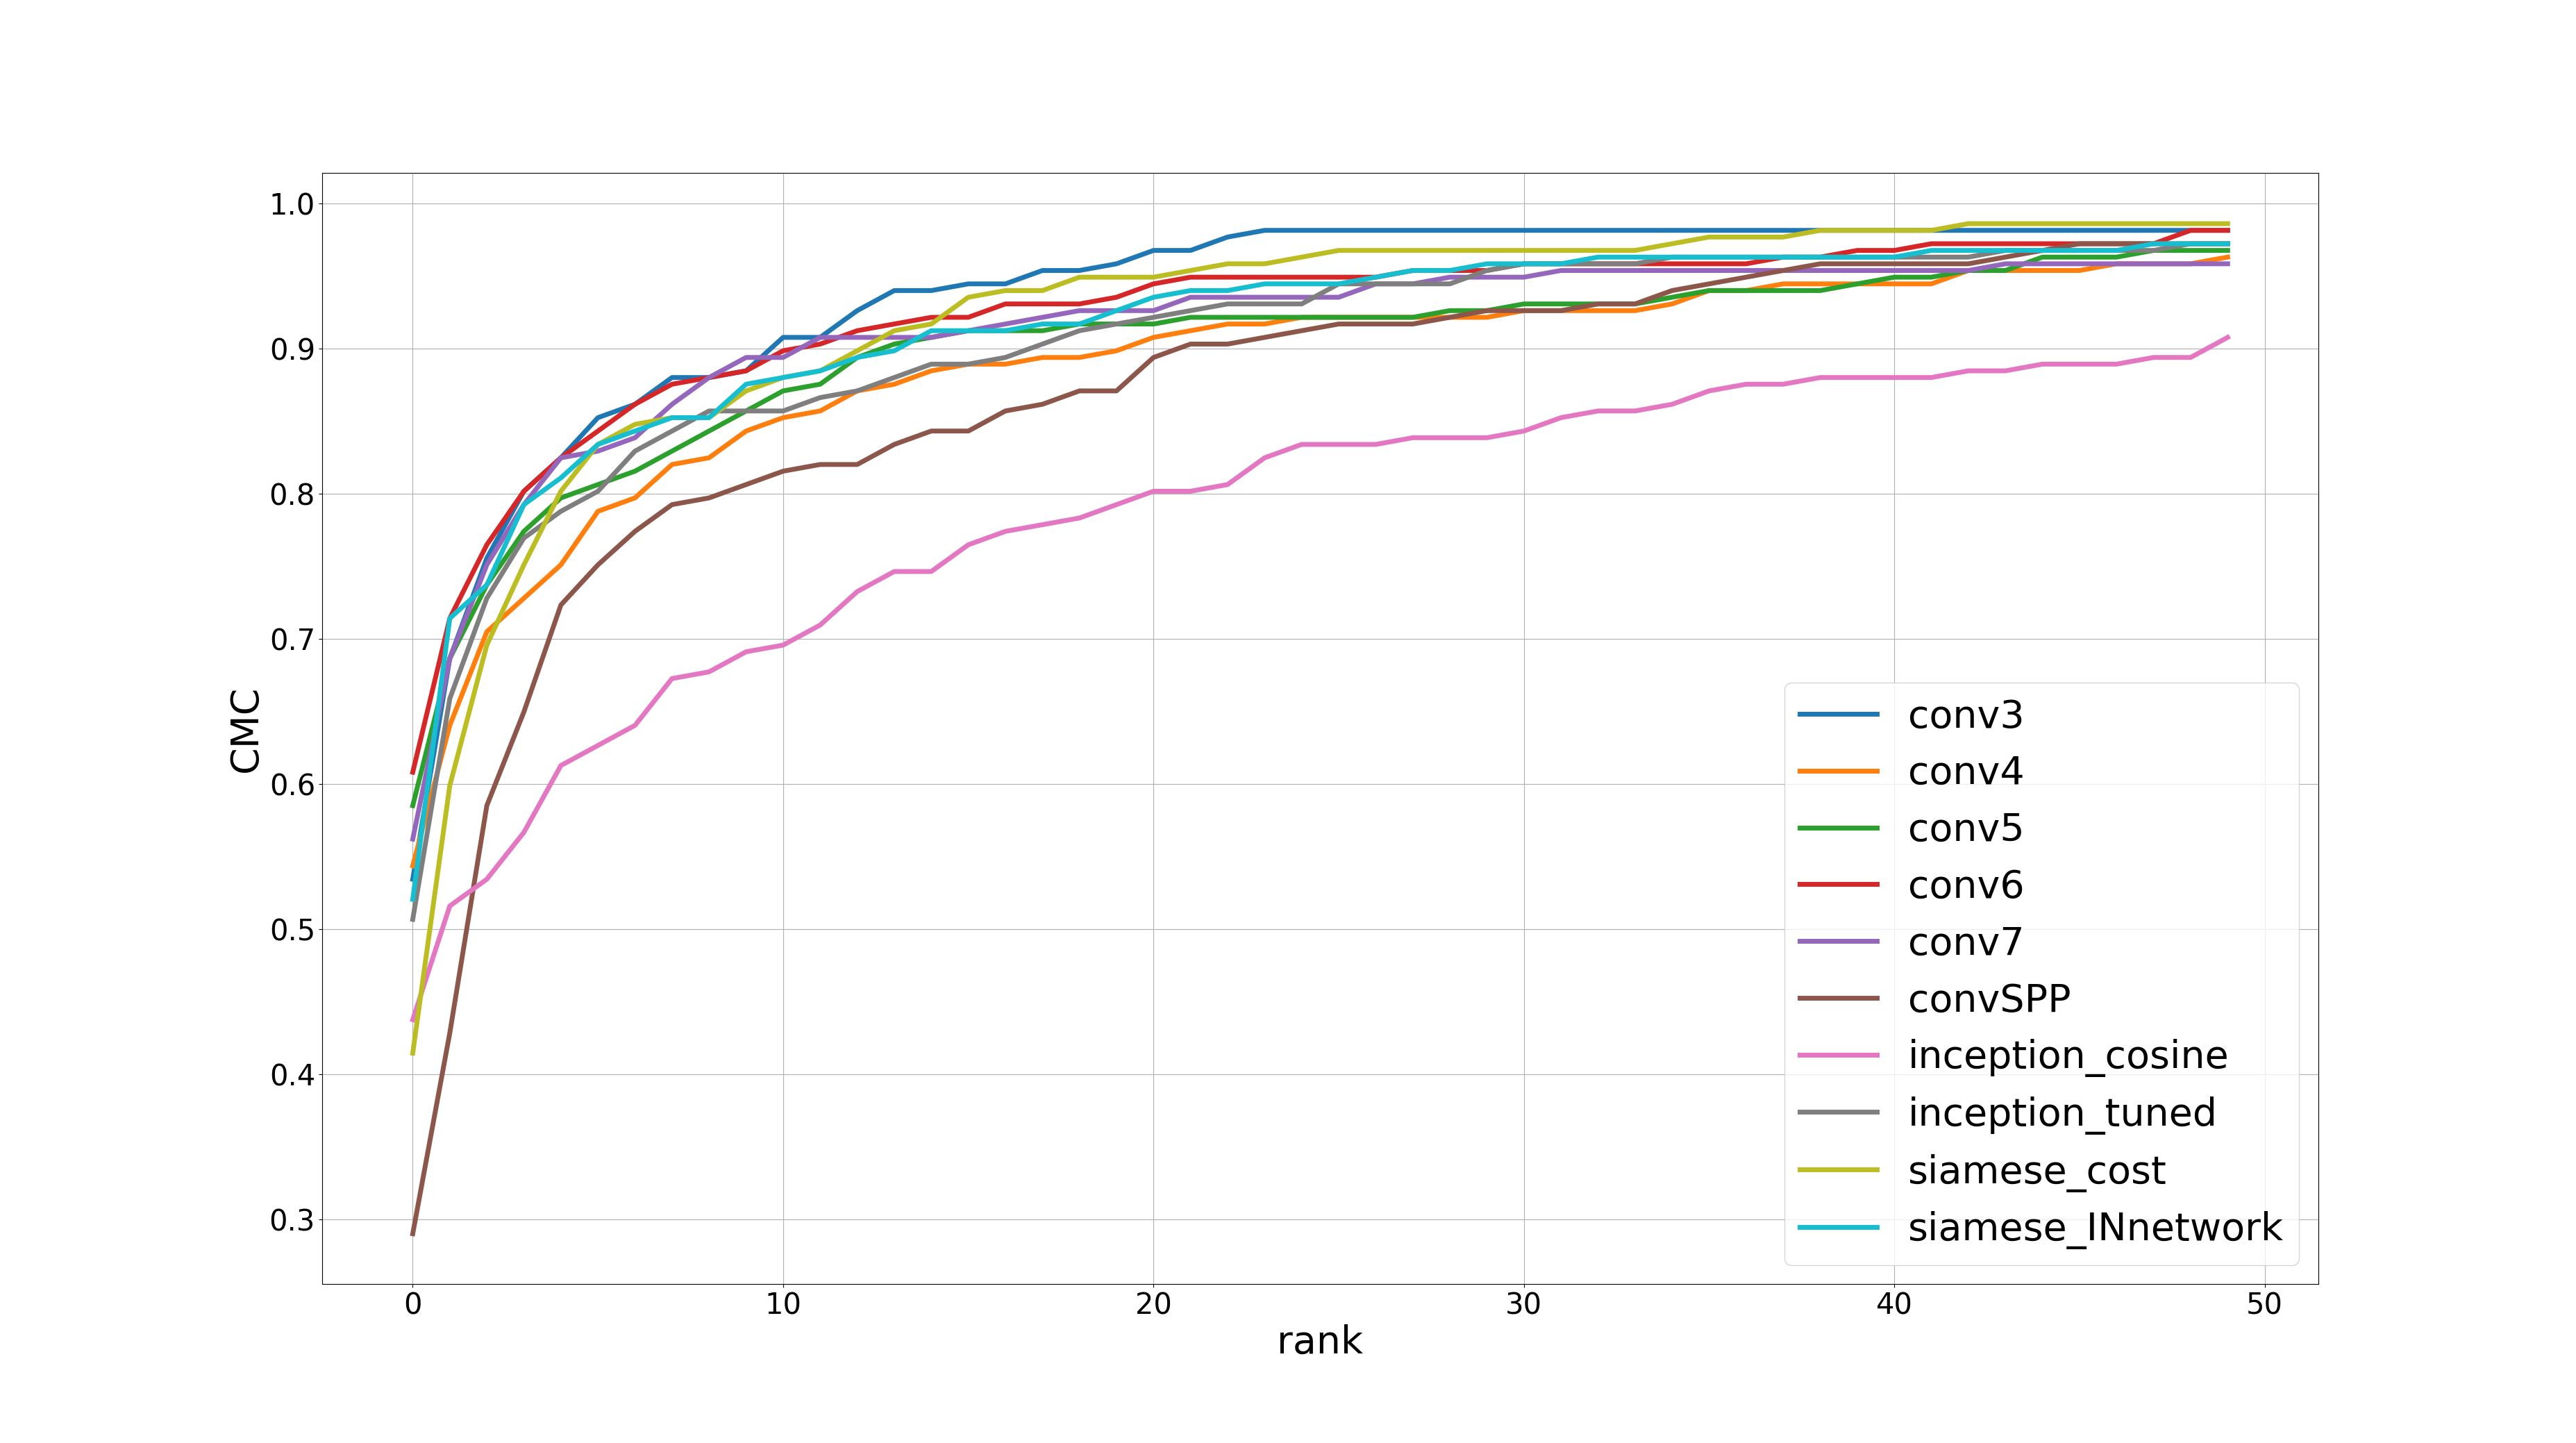
\includegraphics[width=15cm]{siameseDev/cmc2.png}
\caption{CMC plot.} \label{lossesSiam2}
\end{figure}

Also in the figure \ref{lossesSiam3}, we observe the performance against the time consumption. The siamese network with the joint data input with $6$ convolutional layers gets the best balance between performance and execution time. So this was the network included in our robust people tracker, in the reidentification module.

\begin{figure}[hptb]
\centering         
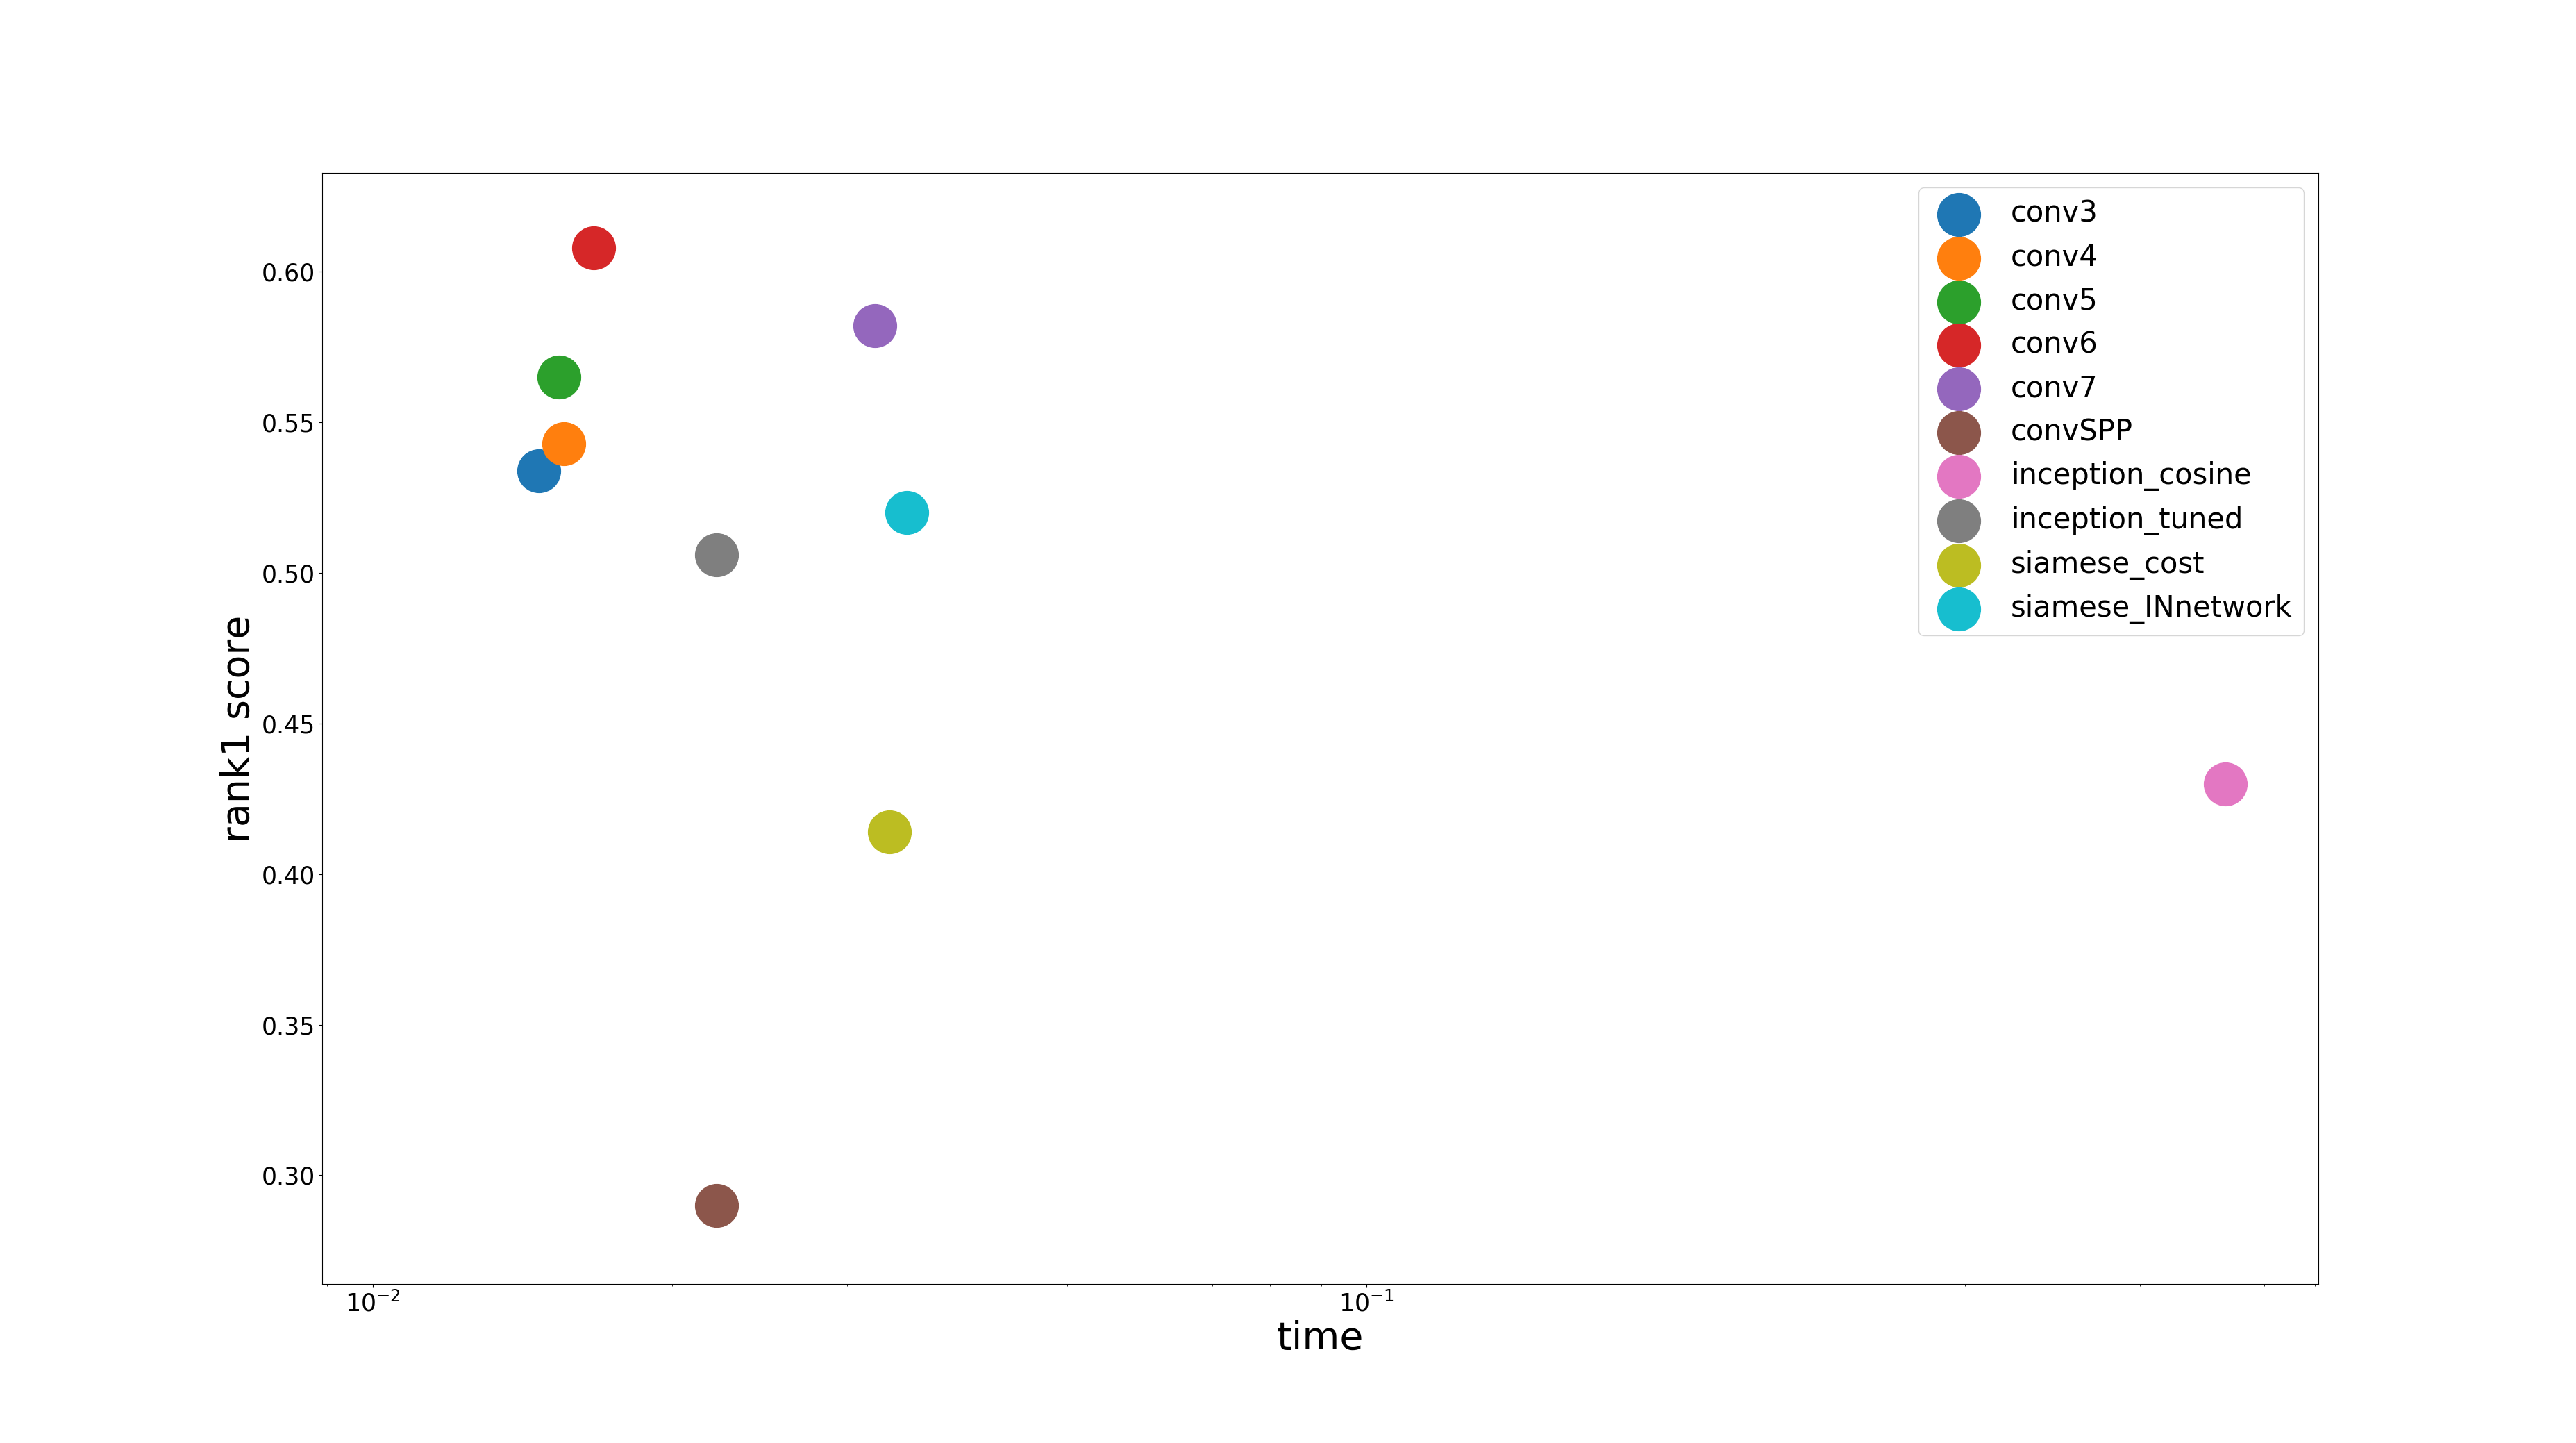
\includegraphics[width=15cm]{siameseDev/graps2.png}
\caption{Performance-timing comparision.} \label{lossesSiam3}
\end{figure}




In the table \ref{tableResultsSiamee}, we studied the impact of the reidentification module, checking the algorithm with and without it. With the reidentification the identity switching (ID's) is reduced around $24 \%$, as can be seen in the numer ob ID's detected in the same dataset.


\begin{table}[H]
\centering

\resizebox{\textwidth}{!}{\begin{tabular}{l|llll|lll|lll|l}
              &  \textbf{GT} & \textbf{MT} & \textbf{PT} & \textbf{ML} & \textbf{FP} & \textbf{FN} & \textbf{IDs} &  \textbf{MOTA} & \textbf{MOTP} &  \textbf{FPS} \\
\textit{Without reidentification}   & 517         & 12           & 180         & 325         & 19098       & 78329       & 827             & 10.3          & 69.1                & 18.2        \\
\textit{With reidentification}  & 517         & 3          & 127         & 387         & 18896       & 78999       & 618                 & 10.8           & 70.3                   & 15.85          \\
  
\end{tabular}}
\caption{Impact of the reidentification module.}
\label{tableResultsSiamee}
\end{table}

\section{Global validation experiments}\label{valdiation}

Once we have explained the experiments for each module, in this sections we show some results of the global system.


\subsection{Typical execution}



Using the code provided by the MOT16 challenge organization, we evaluate our solution on the training set. The evaluation procedure and dataset are explained in previous sections,  \ref{datasetracksEval} and \ref{datasetracks} respectively. The principal measure to compare the algoirthms is the MOTA score, this measure combines three error sources: false positives [FP], missed targets [FN] and identity switches [IDs]. Another measure is the track quality, this measure classifies each trajectory as mostly tracked [MT], partially tracket [PT], and mostly lost [ML]. 


We show the results of our algorithm in the table \ref{tableResults}. We reach 10.8 of MOTA at 15.85 FPS, also around of $24 \%$  of the blobs are partially tracket.




%\begin{table}[H]
%\centering
%
%\resizebox{\textwidth}{!}{\begin{tabular}{l|llll|llll|lll|l}
%              &  \textbf{GT} & \textbf{MT} & \textbf{PT} & \textbf{ML} & \textbf{FP} & \textbf{FN} & \textbf{IDs} & \textbf{FM} & \textbf{MOTA} & \textbf{MOTP} & \textbf{MOTAL} & \textbf{FPS} \\
%\textit{v1}   &  517         & 12          & 180         & 325         & 13339       & 78998       & 827          & 1053        & 9.8           & 69.1          & 6.5            & 18.2         \\
%\textit{v2}  & 517         & 11          & 181         & 325         & 11212       & 75738       & 827          & 1056        & 9.7           & 67.3          & 6.1            & 9.0          \\
%\textit{v3}   & 517         & 3           & 127         & 387         & 13373       & 78999       & 618          & 936         & 10.8          & 70.3          & 7.5            & 15.85        \\
%\textit{SOTA} & 517         & 92          & 219         & 206         & 5333        & 86795       & 391          & -           & 49.3          & 79.0          & -              & 0.8         
%\end{tabular}}
%\caption{Results algorithm global.}
%\label{tableResults}
%\end{table}


\begin{table}[H]
\centering

\resizebox{\textwidth}{!}{\begin{tabular}{l|llll|lll|ll|l}
              &  \textbf{GT} & \textbf{MT} & \textbf{PT} & \textbf{ML} & \textbf{FP} & \textbf{FN} & \textbf{IDs}  & \textbf{MOTA} & \textbf{MOTP}  & \textbf{FPS} \\
\textit{Our algorithm}   & 517         & 3           & 127         & 387         & 18896       & 78999       & 618             & 10.8          & 70.3                & 15.85        \\
\end{tabular}}
\caption{Results of our algorithm.}
\label{tableResults}
\end{table}





%According to this results, we decided to do not use the forward-backward method, due for its high computation demands and its limited improvement. Also, we observe the usage of a mechanism of re-identification increment the MOTA performance, so the overall performance of the detector, with the cost of increase the running time. This improvement come from the reduction in around $24 \%$ the identity switching (ID's) parameter. From this statistical comparision we discard the forward-backward method and it is worth to use the person re-identification module.

In addition, we show the results for each sequences, we can observe the results in the table \ref{tableResultsSequences}. 


%\begin{table}[]
%\centering
%\caption{My caption}
%\begin{tabular}{lllll}
%Name        & FPS & Resolution & Density & Description                        \\ \hline
%\textit{02} & 30  & 1920x1080  & 29.7    & Fixed camera, low angle            \\
%\textit{04} & 30  & 1920x1080  & 45.3    & Fixed camera, elevated viewpoint   \\
%\textit{05} & 14  & 640x480    & 8.1     & Moving camera, low angle           \\
%\textit{09} & 30  & 1920x1080  & 10      & Fixed camera, low angle            \\
%\textit{10} & 30  & 1920x1080  & 18.8    & Moving camera, low angle           \\
%\textit{11} & 30  & 1920x1080  & 10.2    & Moving camera, low angle           \\
%\textit{13} & 25  & 1920x1080  & 15.3    & Moving camera, elevated  viewpoint
%\end{tabular}
%\label{my-label}
%\end{table}


\begin{table}[!]
\centering

\resizebox{\textwidth}{!}{\begin{tabular}{l|llll|lll|ll|l}
                & \textbf{GT} & \textbf{MT} & \textbf{PT} & \textbf{ML} & \textbf{FP} & \textbf{FN} & \textbf{IDs}  & \textbf{MOTA} & \textbf{MOTP}  & \textbf{FPS} \\
\textit{02}     & 54          & 0           & 13          & 41          & 2181        & 15526       & 113                  & 0.1           & 67.1           & 9.02         \\
\textit{04}     & 83          & 0           & 41          & 42          & 5495        & 33980             & 290         & 16.6          & 71.1          &  12.3         \\
\textit{05}              & 125         & 3           & 43          & 79          & 28571       & 4713              & 109         & -12.2         & 67.8          & 17.94        \\
\textit{09}              & 25          & 1           & 19          & 5           & 932         & 3225              & 71          & 19.7          & 62           & 10.52        \\
\textit{10}              & 54          & 0           & 4           & 50          & 404         & 11647       & 81                    & 1.5           & 68.4                 & 14.23        \\
\textit{11}              & 69          & 0           & 16          & 53          & 948         & 7366        & 72                   & 8.6           & 71.4                 & 17.49        \\
\textit{13}              & 107         & 0           & 9           & 98          & 1315        & 10743       & 32                    & -5.6          & 67.1                  & 20.5         \\ \hline
\textit{Global} & 517         & 3           & 127         & 387         & 18896       & 78999       & 618                  & 10.8          & 70.3           & 15.85       
\end{tabular}}
\caption{Results algorithm by sequences.}
\label{tableResultsSequences}
\end{table}


The algorithm gets the best performance on sequences with a fixed camera from an elevated view point and a low angle recording and close targets like sequences $4,9 $, and $11$. In the figures \ref{seq1} and \ref{seq2} we can observe a snapshot of these sequences.



\begin{figure}[H]
		
\centering

\subfigure[Our algorithm]{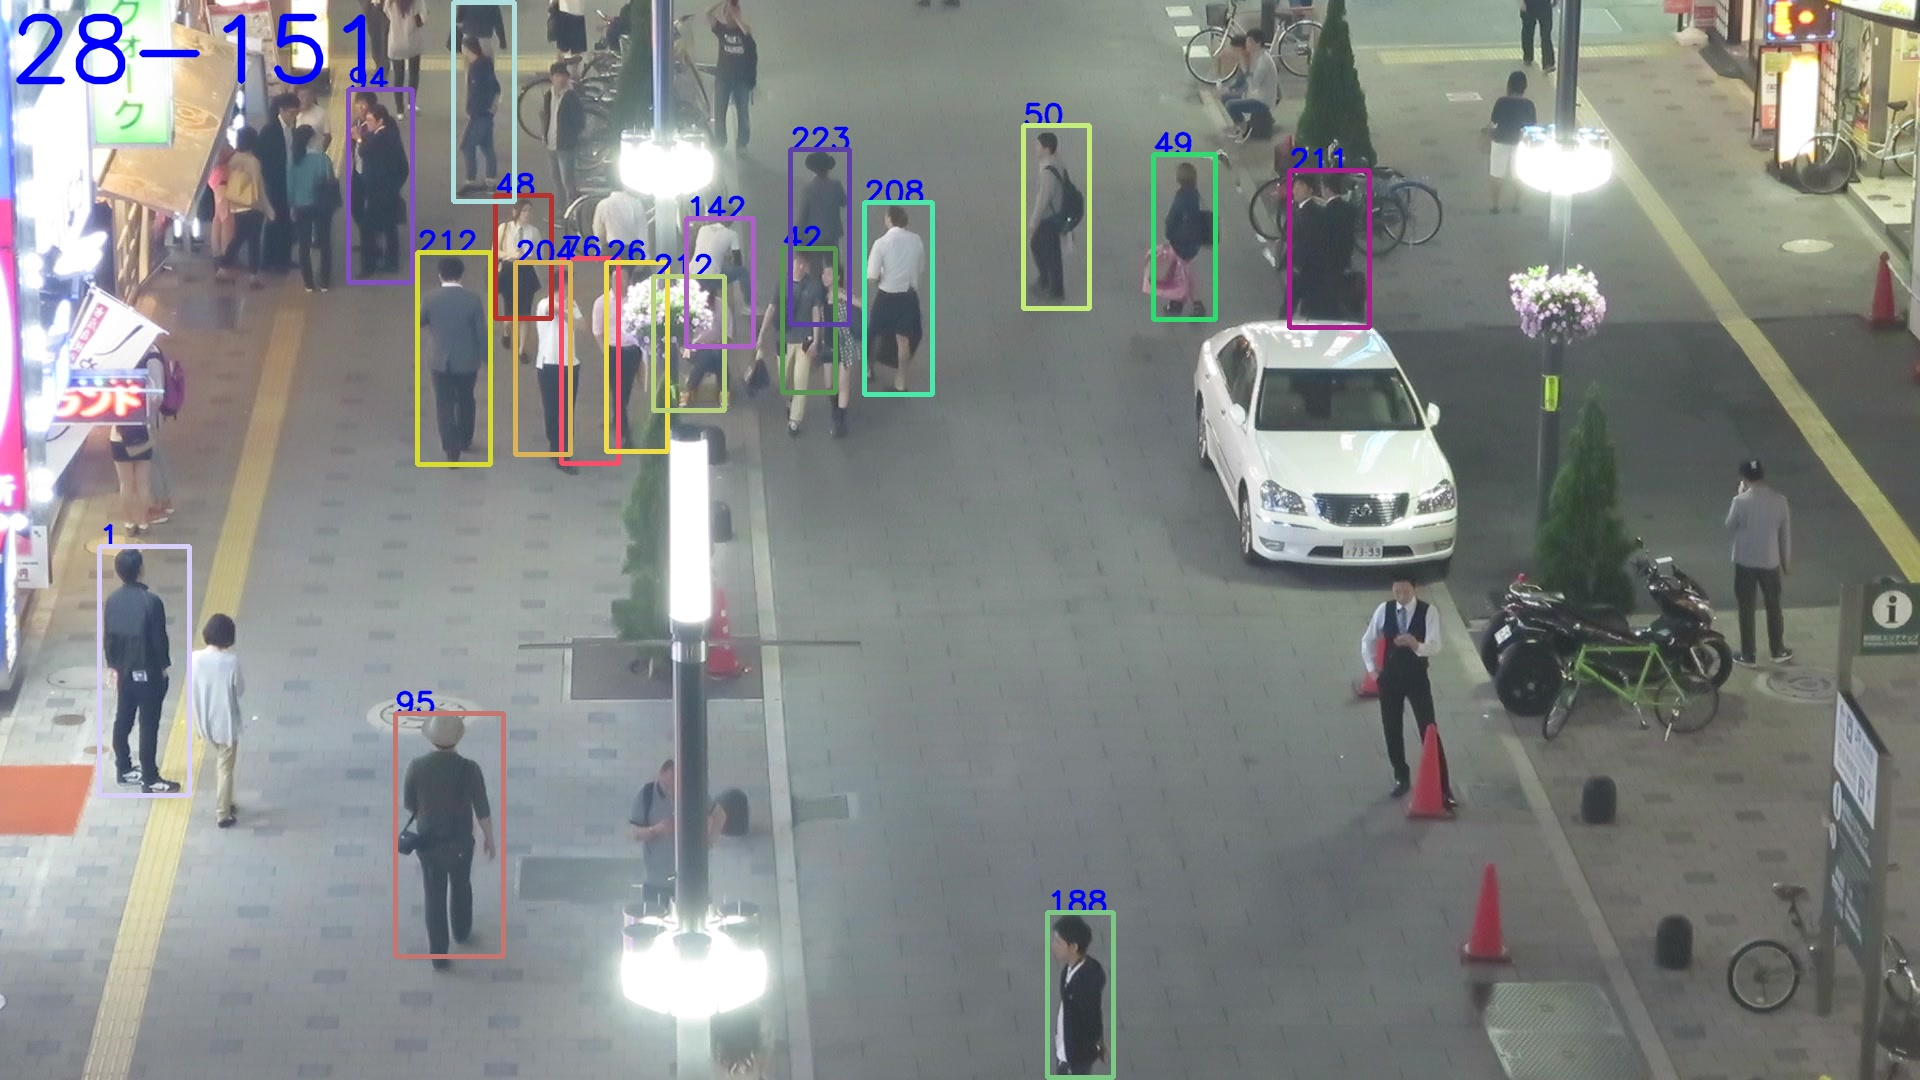
\includegraphics[width=7cm]{comparision/our04.jpg}}
\subfigure[Ground truth]{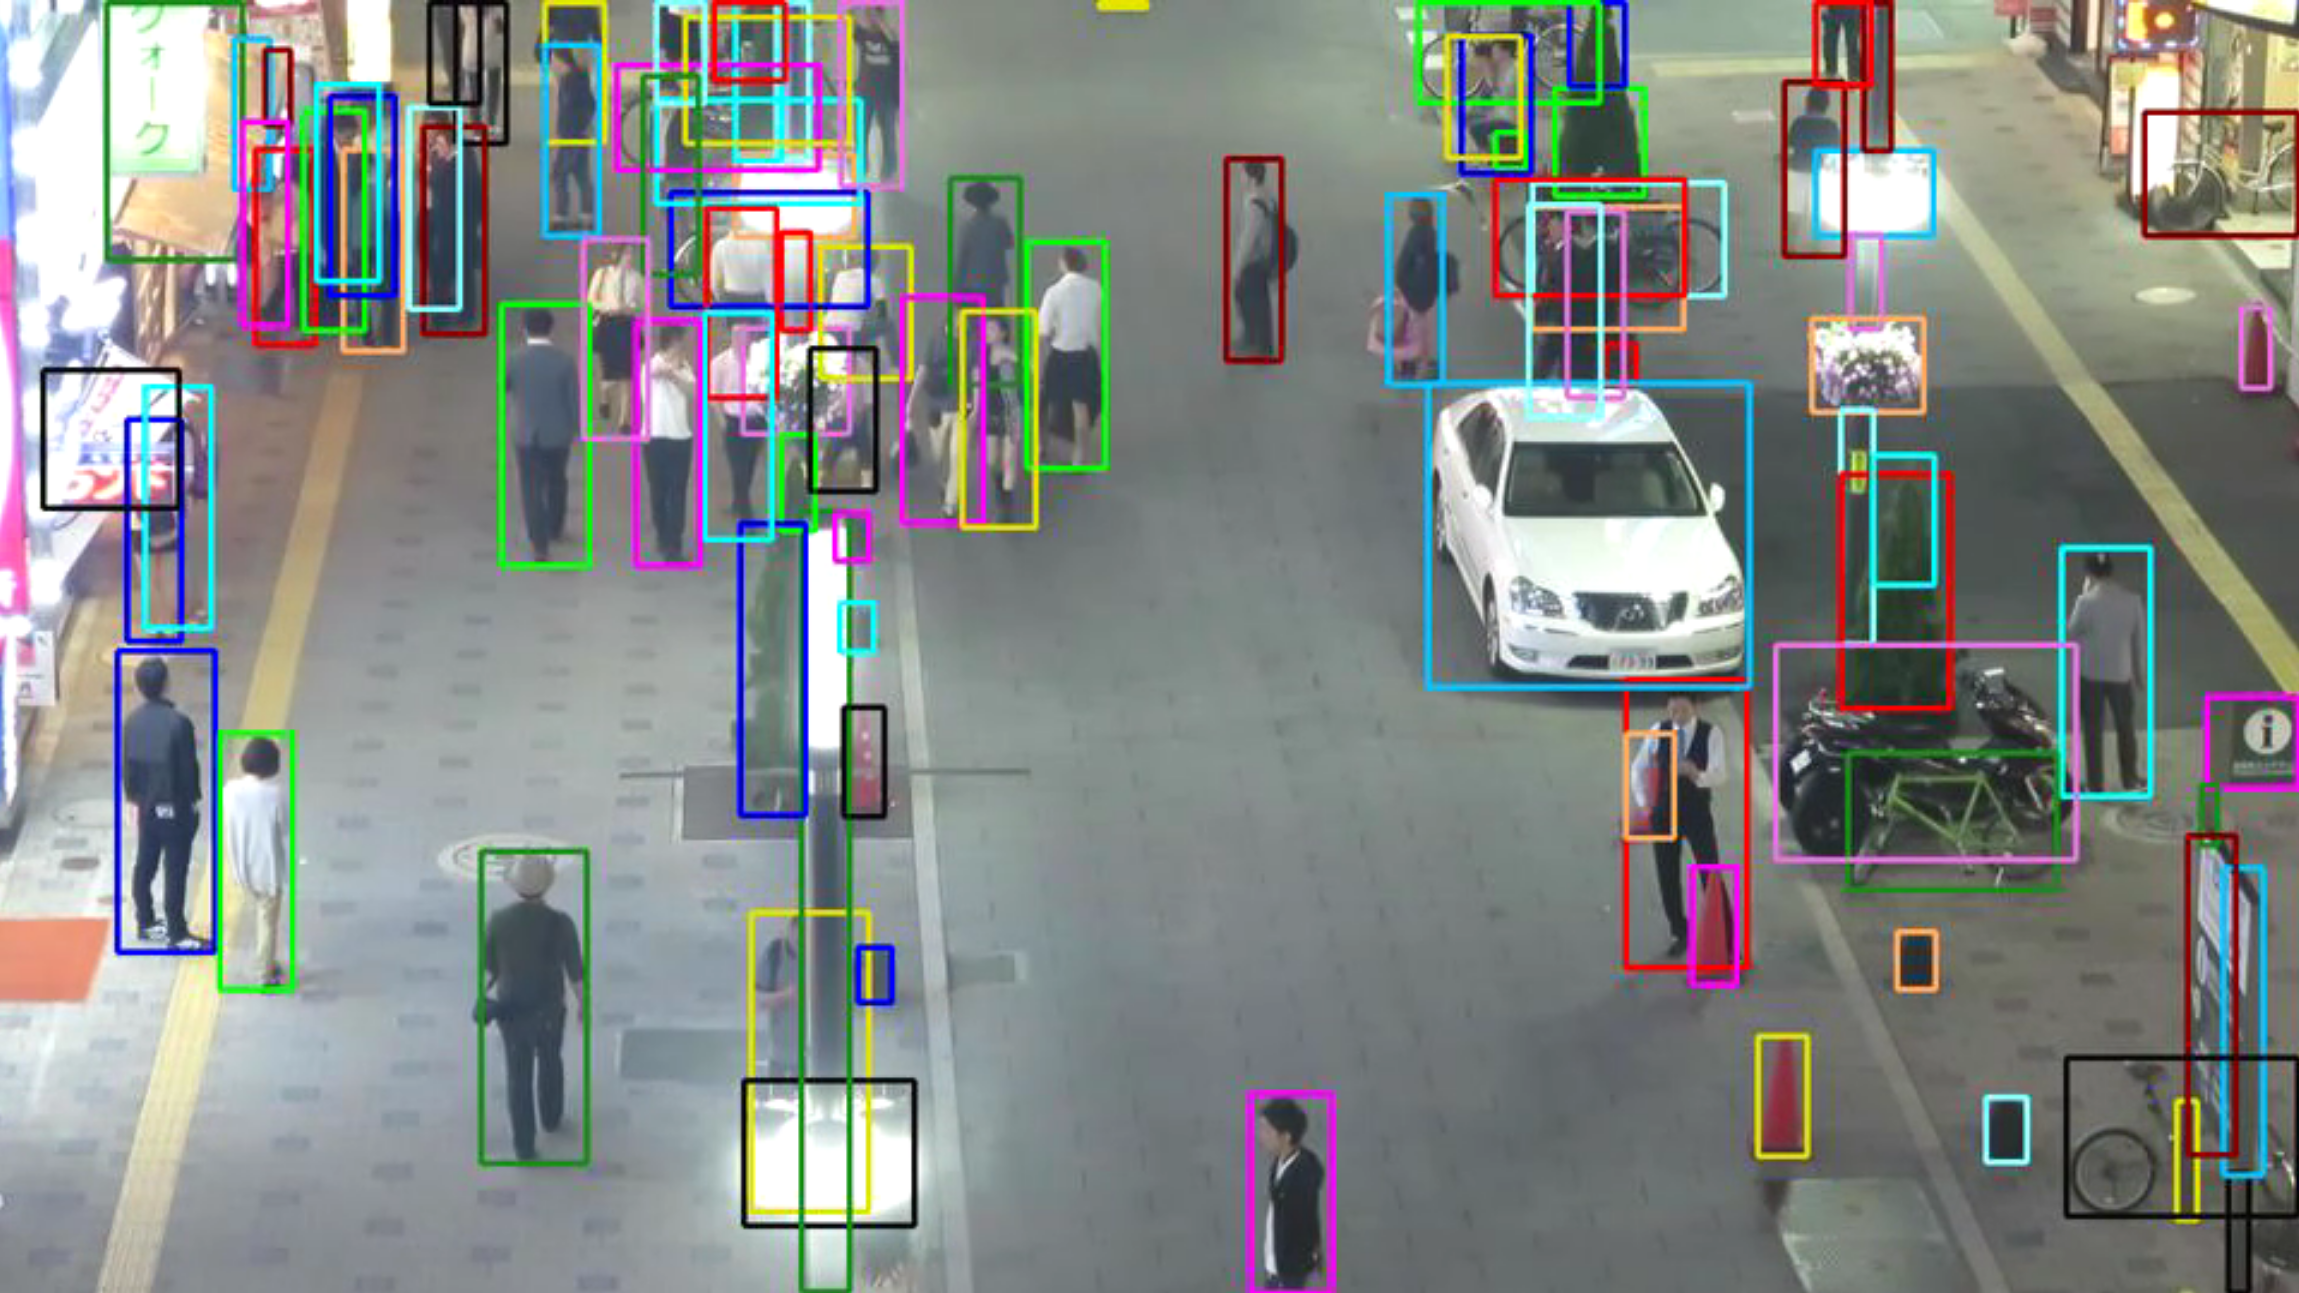
\includegraphics[width=7cm]{comparision/gt04.png}}\\
\caption{Comparision between our algorithm with MOT-04 ground truth.}
\label{seq1}
\end{figure}


\begin{figure}[H]
		
\centering

\subfigure[Our algorithm]{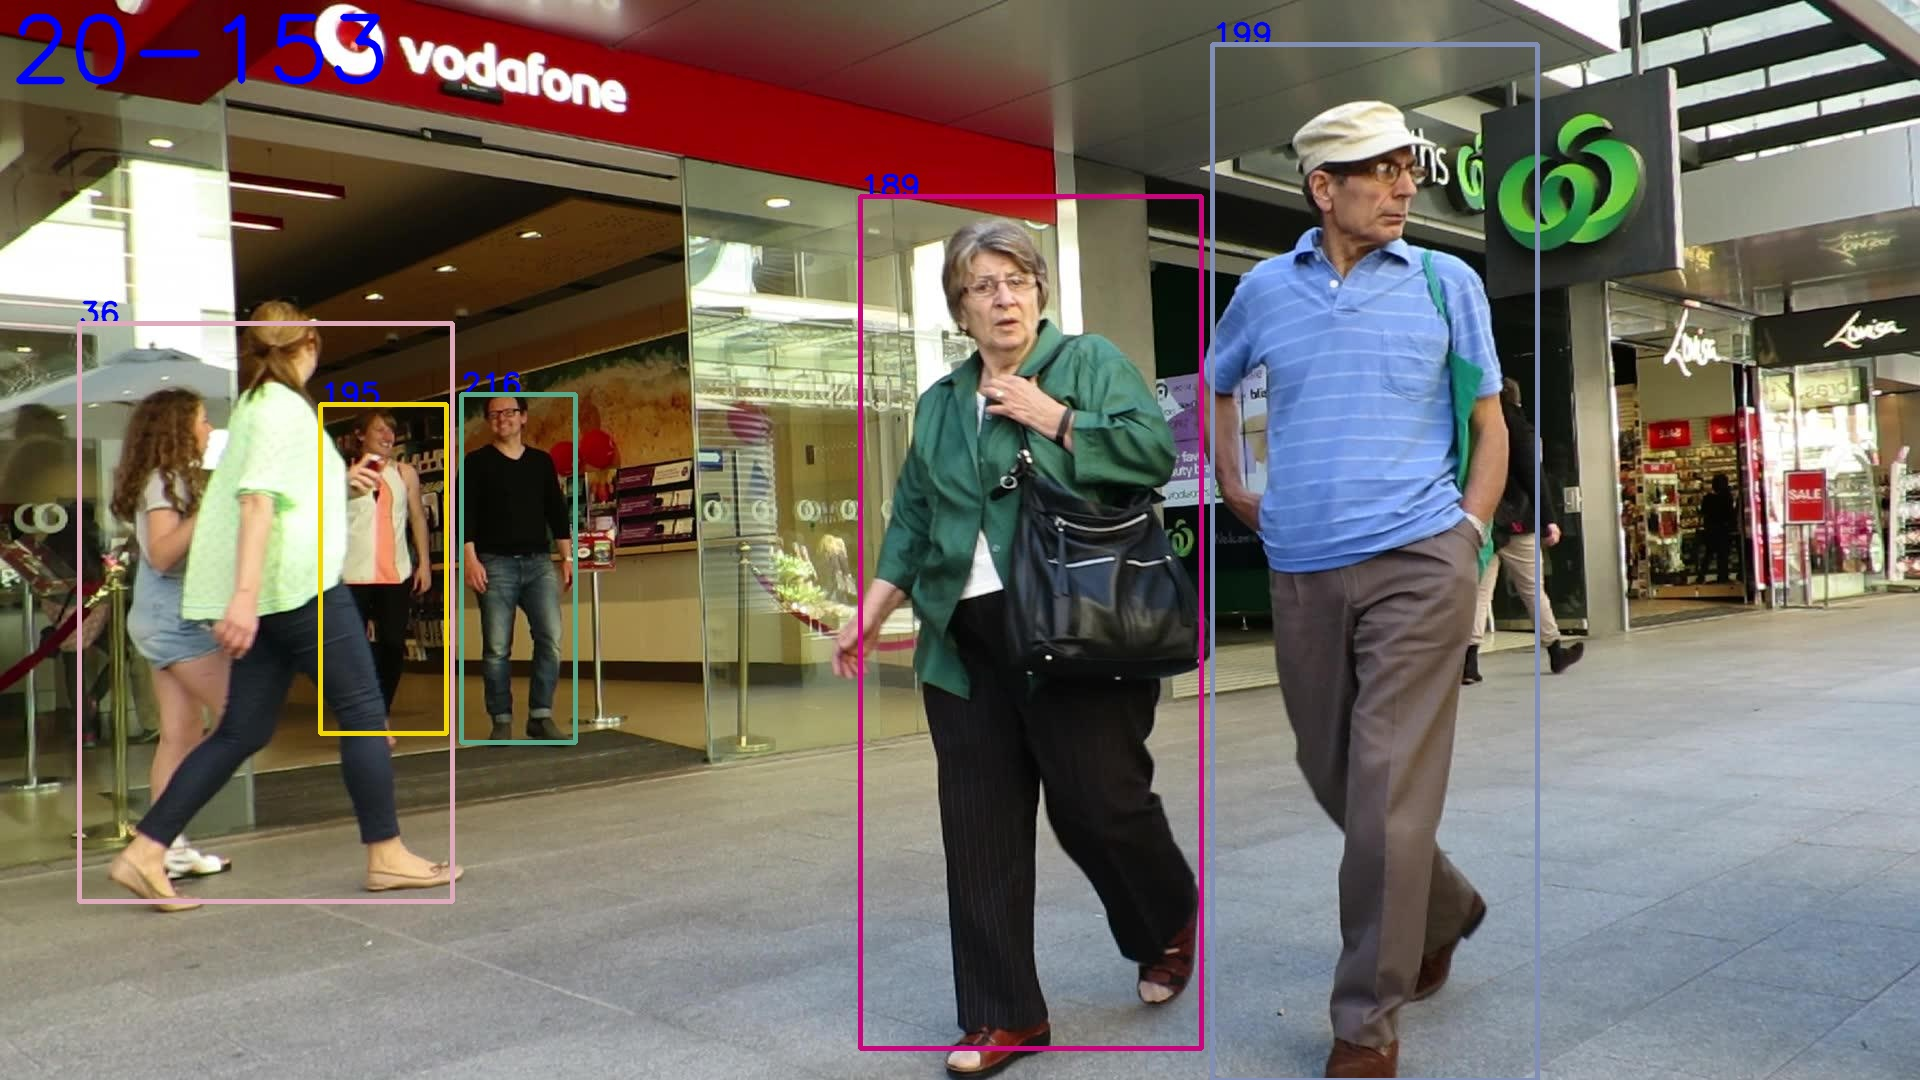
\includegraphics[width=7cm]{comparision/our09.jpg}}
\subfigure[Ground truth]{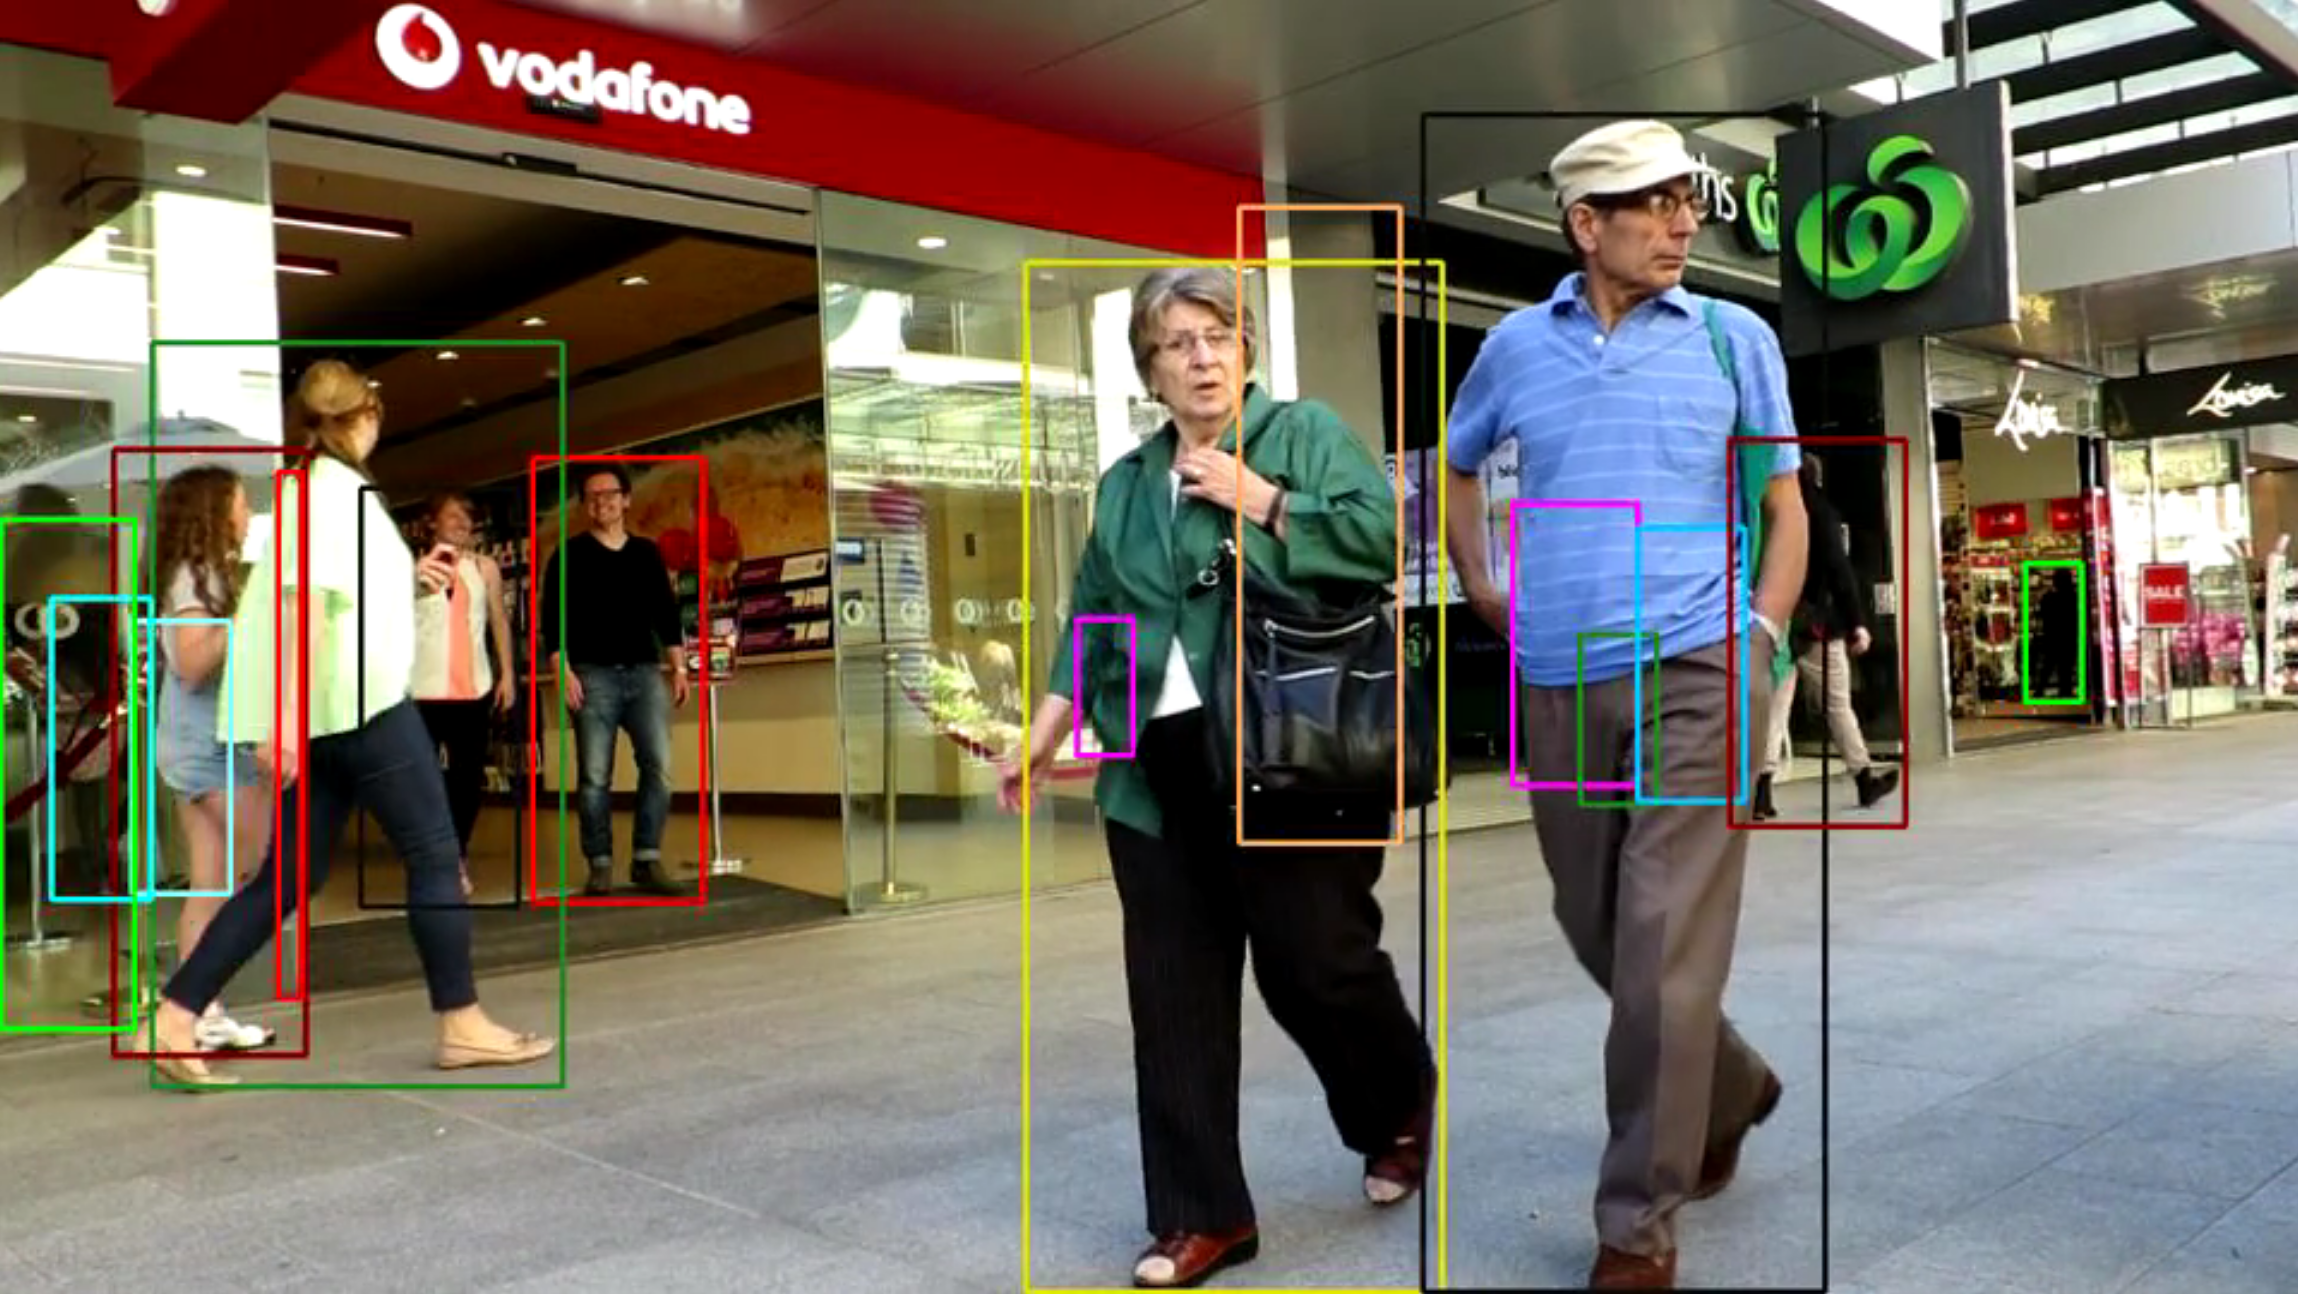
\includegraphics[width=7cm]{comparision/gt09.png}}\\
\caption{Comparision between our algorithm with MOT-09 ground truth.}
\label{seq2}
\end{figure}


In contrast, our algorithm struggles in sequences with low resolution like sequences $5$, and when the targets are away from the camera like $13$. In the figure \ref{seq3} and \ref{seq4} we can observe a snapshot of these sequences.


\begin{figure}[H]
		
\centering

\subfigure[Our algorithm]{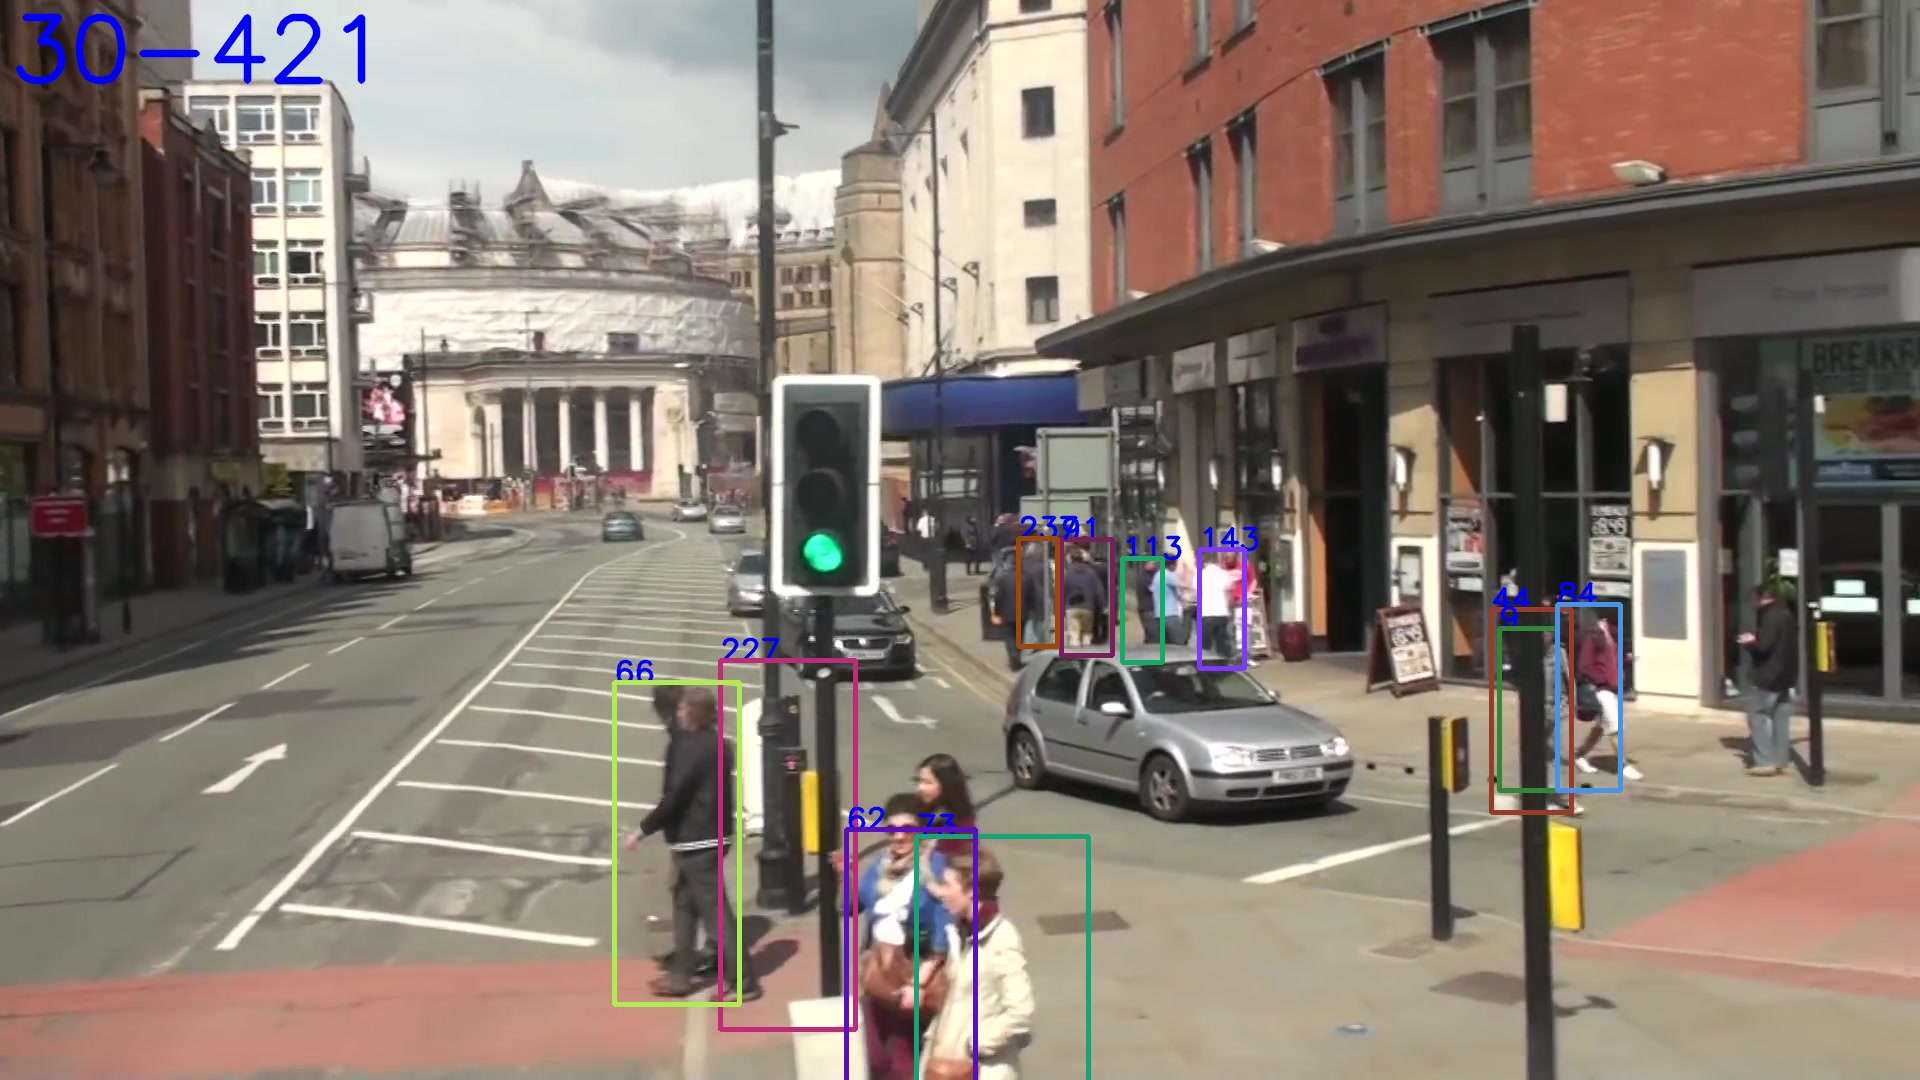
\includegraphics[width=7cm]{comparision/our13.jpg}}
\subfigure[Ground truth]{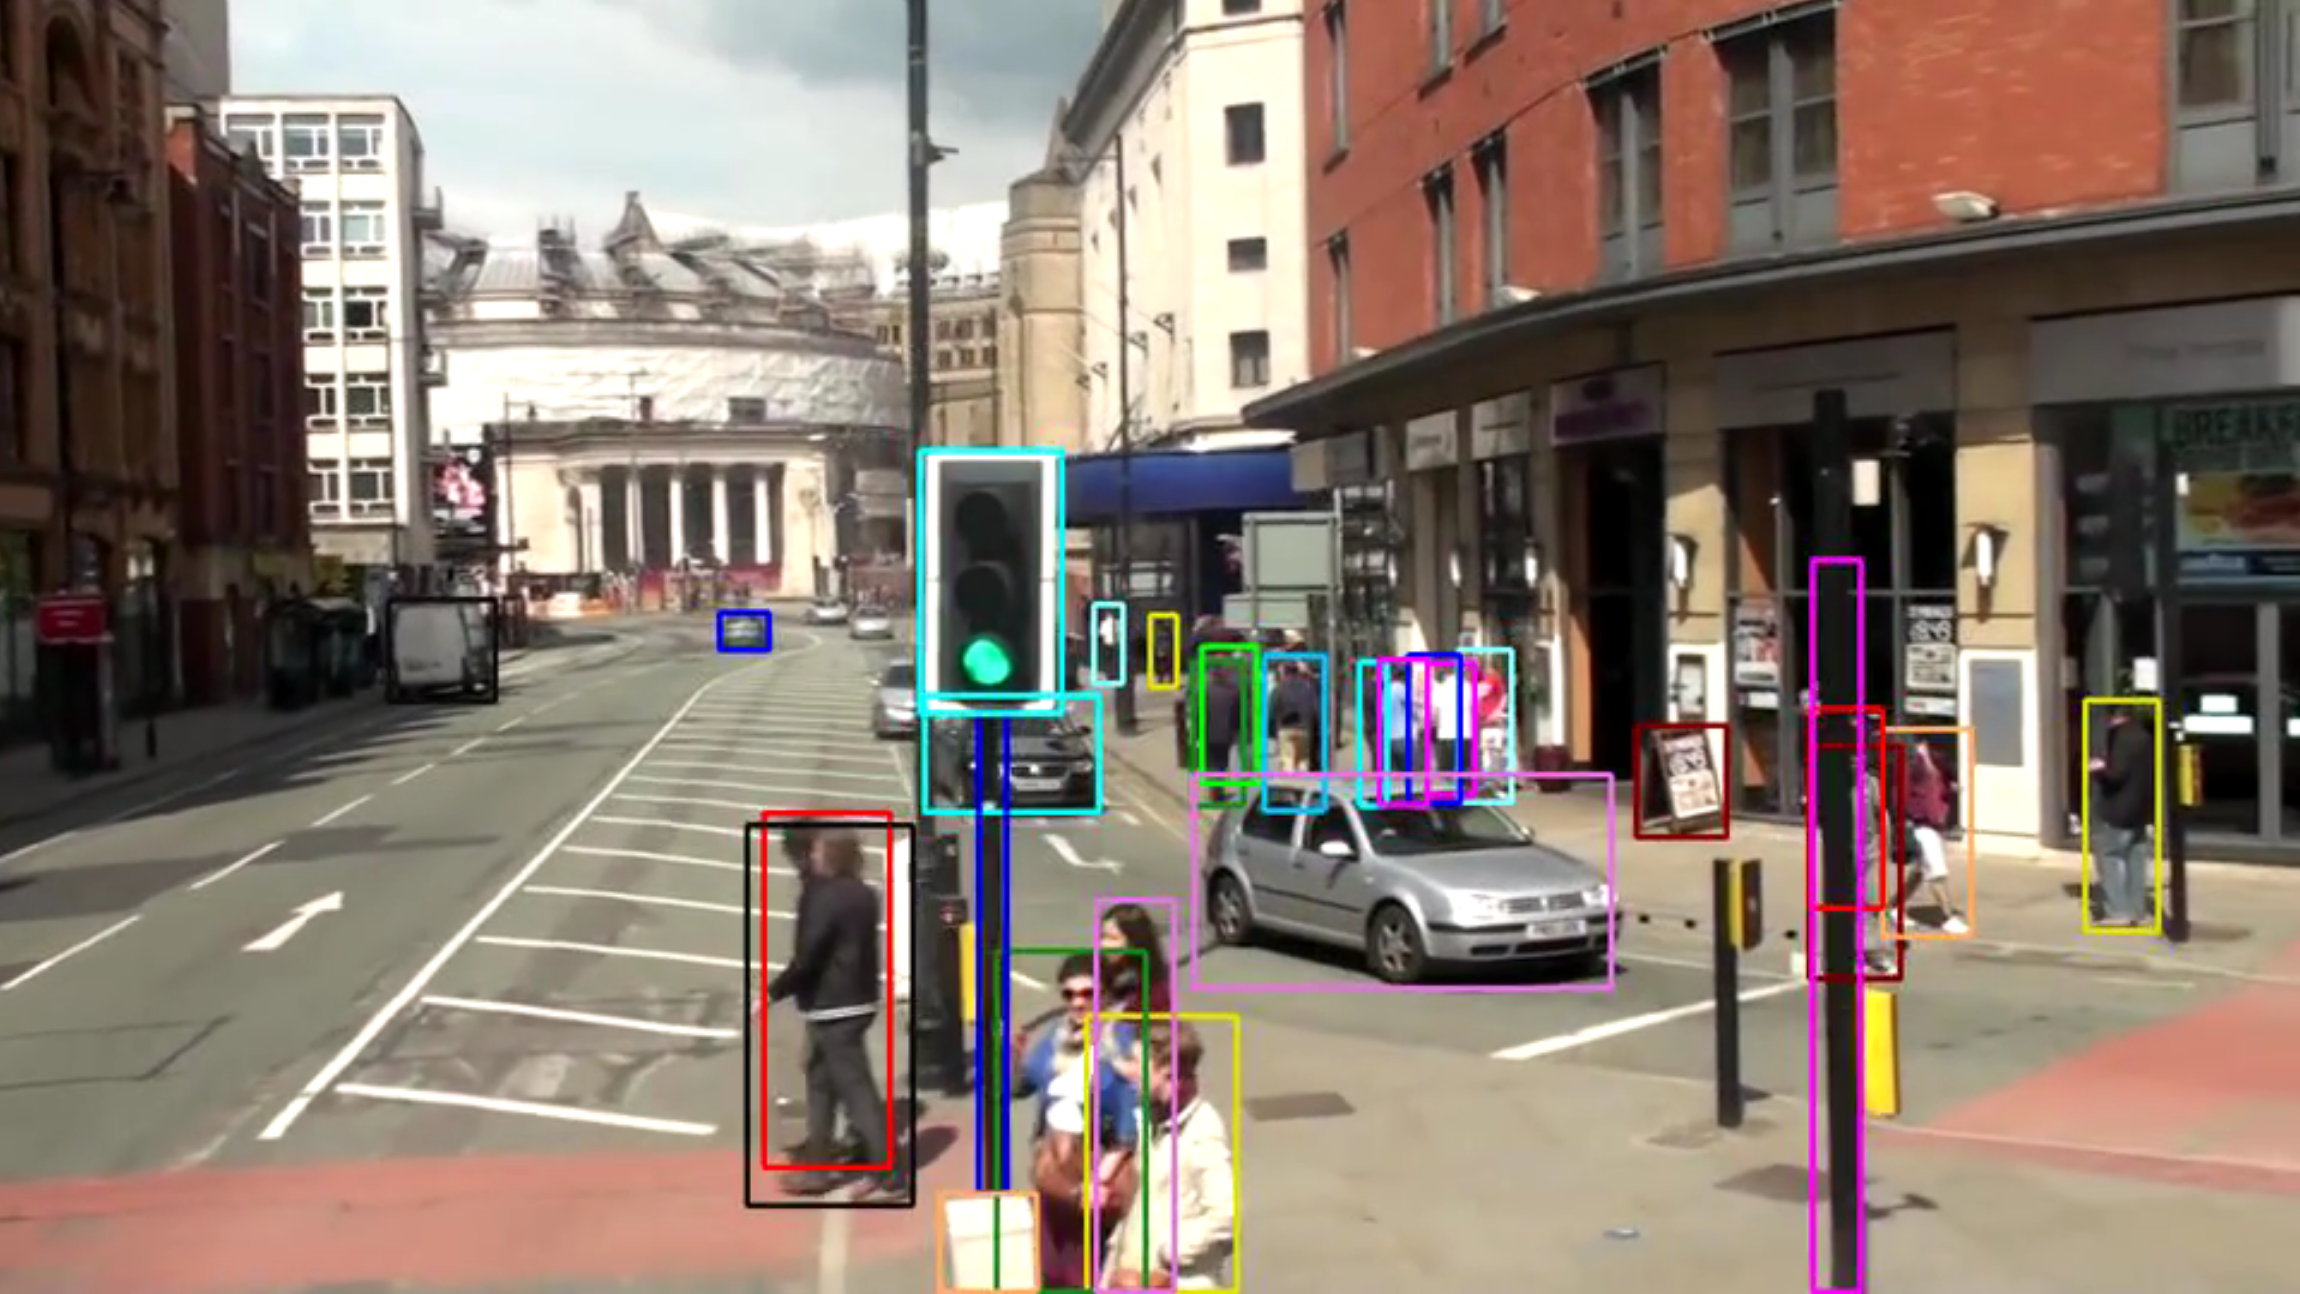
\includegraphics[width=7cm]{comparision/gt13.png}}\\
\caption{Comparison between our algorithm with MOT-13 ground truth}
\label{seq3}
\end{figure}


\begin{figure}[H]
		
\centering

\subfigure[Our algorithm]{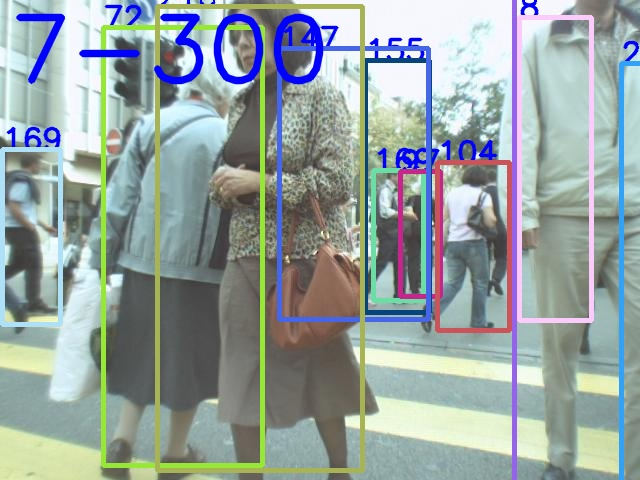
\includegraphics[width=7cm]{comparision/our05.jpg}}
\subfigure[Ground truth]{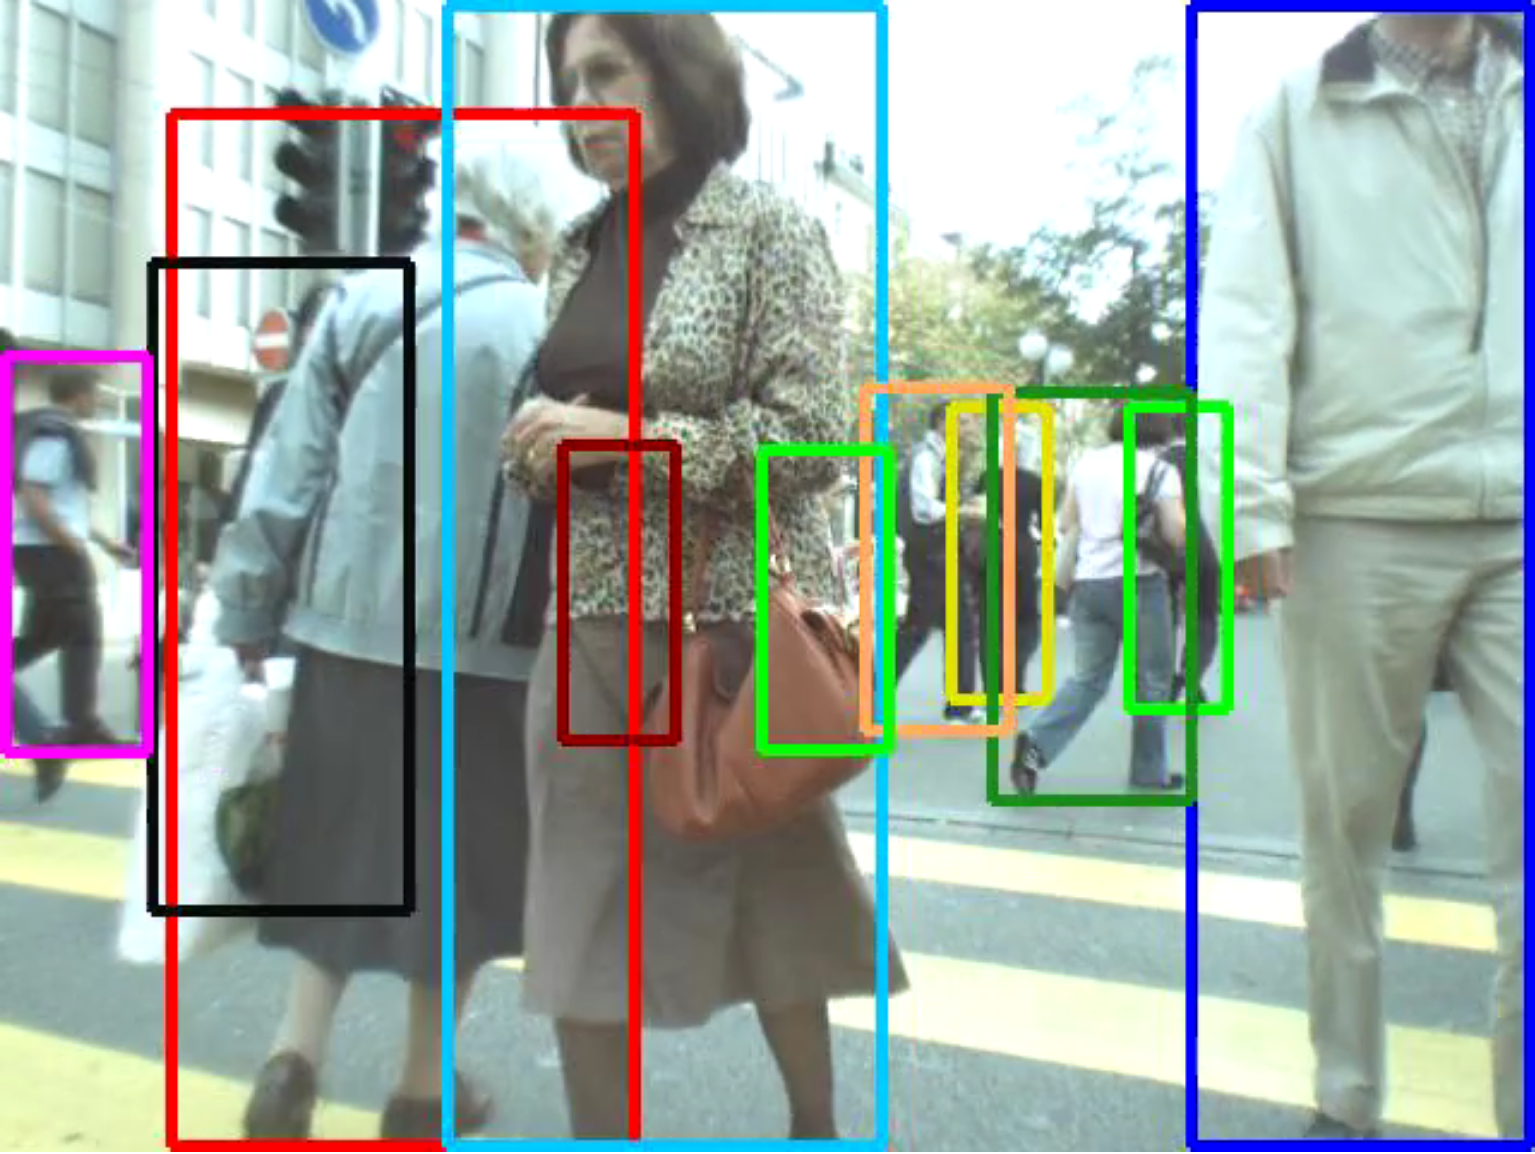
\includegraphics[width=7cm]{comparision/gt05.png}}\\
\caption{Comparison between our algorithm with MOT-05 ground truth}
\label{seq4}
\end{figure}



We did not evaluate on the test set because the ground truth it is not provided by the organization. You have to submit yours results on their website to get an evaluation on this set, but the website it is blocked because an upcoming conference. Evaluating our results on the test set will not reveal any furhter analyse because they are different cuts of the same video sequences


\subsection{Comparison with other algorithms}

%\begin{table}[H]
%\centering
%
%\resizebox{\textwidth}{!}{\begin{tabular}{l|llll|llll|lll|l}
%              &  \textbf{GT} & \textbf{MT} & \textbf{PT} & \textbf{ML} & \textbf{FP} & \textbf{FN} & \textbf{IDs} & \textbf{FM} & \textbf{MOTA} & \textbf{MOTP} & \textbf{MOTAL} & \textbf{FPS} \\
%\textit{Our}   & 517         & 3           & 127         & 387         & 13373       & 78999       & 618          & 936         & 10.8          & 70.3          & 7.5            & 15.85        \\
%\textit{SOTA} & 517         & 92          & 219         & 206         & 5333        & 86795       & 391          & -           & 49.3          & 79.0          & -              & 0.8         
%\end{tabular}}
%\caption{Results algorithm global.}
%\label{tableResults}
%\end{table}

We have compared our algorithm with the MOT16 leaderboard \cite{motResults}, we only include the algorithms which belong to a research paper, in the table \ref{tableSOTatomeu} and the figure \ref{experimenComp} we can observe those results. We observe that these algorithms overtake our solution on the MOTA measure but we pass them in processing speed, even their processing speed parameter does not include the execution of their detector.

These algorithms are focused on solving the data association module from the tracking-by-detection paradigm, to do so they have access to the detection at each frame. They focus on how to link those detections and do not consider the processing speed. Instead, we were focused on how to develop a tracking-by-detection with neural networks on real time.
 

\begin{table}[!]
\centering
\begin{tabular}{l|llll|lll|ll|l}
                 & \textbf{GT} & \textbf{MT} & \textbf{PT} & \textbf{ML} & \textbf{FP} & \textbf{FN} & \textbf{IDs} & \textbf{MOTA} & \textbf{MOTP} & \textbf{FPS} \\
\textit{DP\_NMS} \cite{dpnms} & 517         & 28          & 169         & 320         & 1123        & 121578      & 972          & 32.2          & 76.4          & 212.6        \\
\textit{CEM} \cite{cem}             & 517         & 40          & 198         & 279         & 6837        & 114322      & 642          & 33.2          & 75.8          & 0.3          \\
\textit{SMOT} \cite{smot}    & 517         & 22          & 253         & 242         & 17426       & 107552      & 3108         & 29.7          & 76.3          & 0.2          \\
\textit{LP2D} \cite{mot}   & 517         & 44          & 211         & 262         & 5084        & 111163      & 915          & 35.7          & 75.8          & 49.3         \\
\textit{MDPNN} \cite{savaresee}  & 517         & 72          & 287         & 215         & 2681        & 92856       & 774          & 47.2          & 75.8          & 1.0          \\
\textit{LMP}  \cite{lmp}   & 517         & 98          & 222         & 197         & 8886        & 85487       & 852          & 48.8          & 79            & 0.5          \\
\textit{Our method}     & 517         & 3           & 127         & 387         & 18896       & 78999       & 618          & 10.8          & 70.3          & 15.85       
\end{tabular}
\caption{Comprarison with the MOT's results}
\label{tableSOTatomeu}
\end{table}



\begin{figure}[!]
\centering         
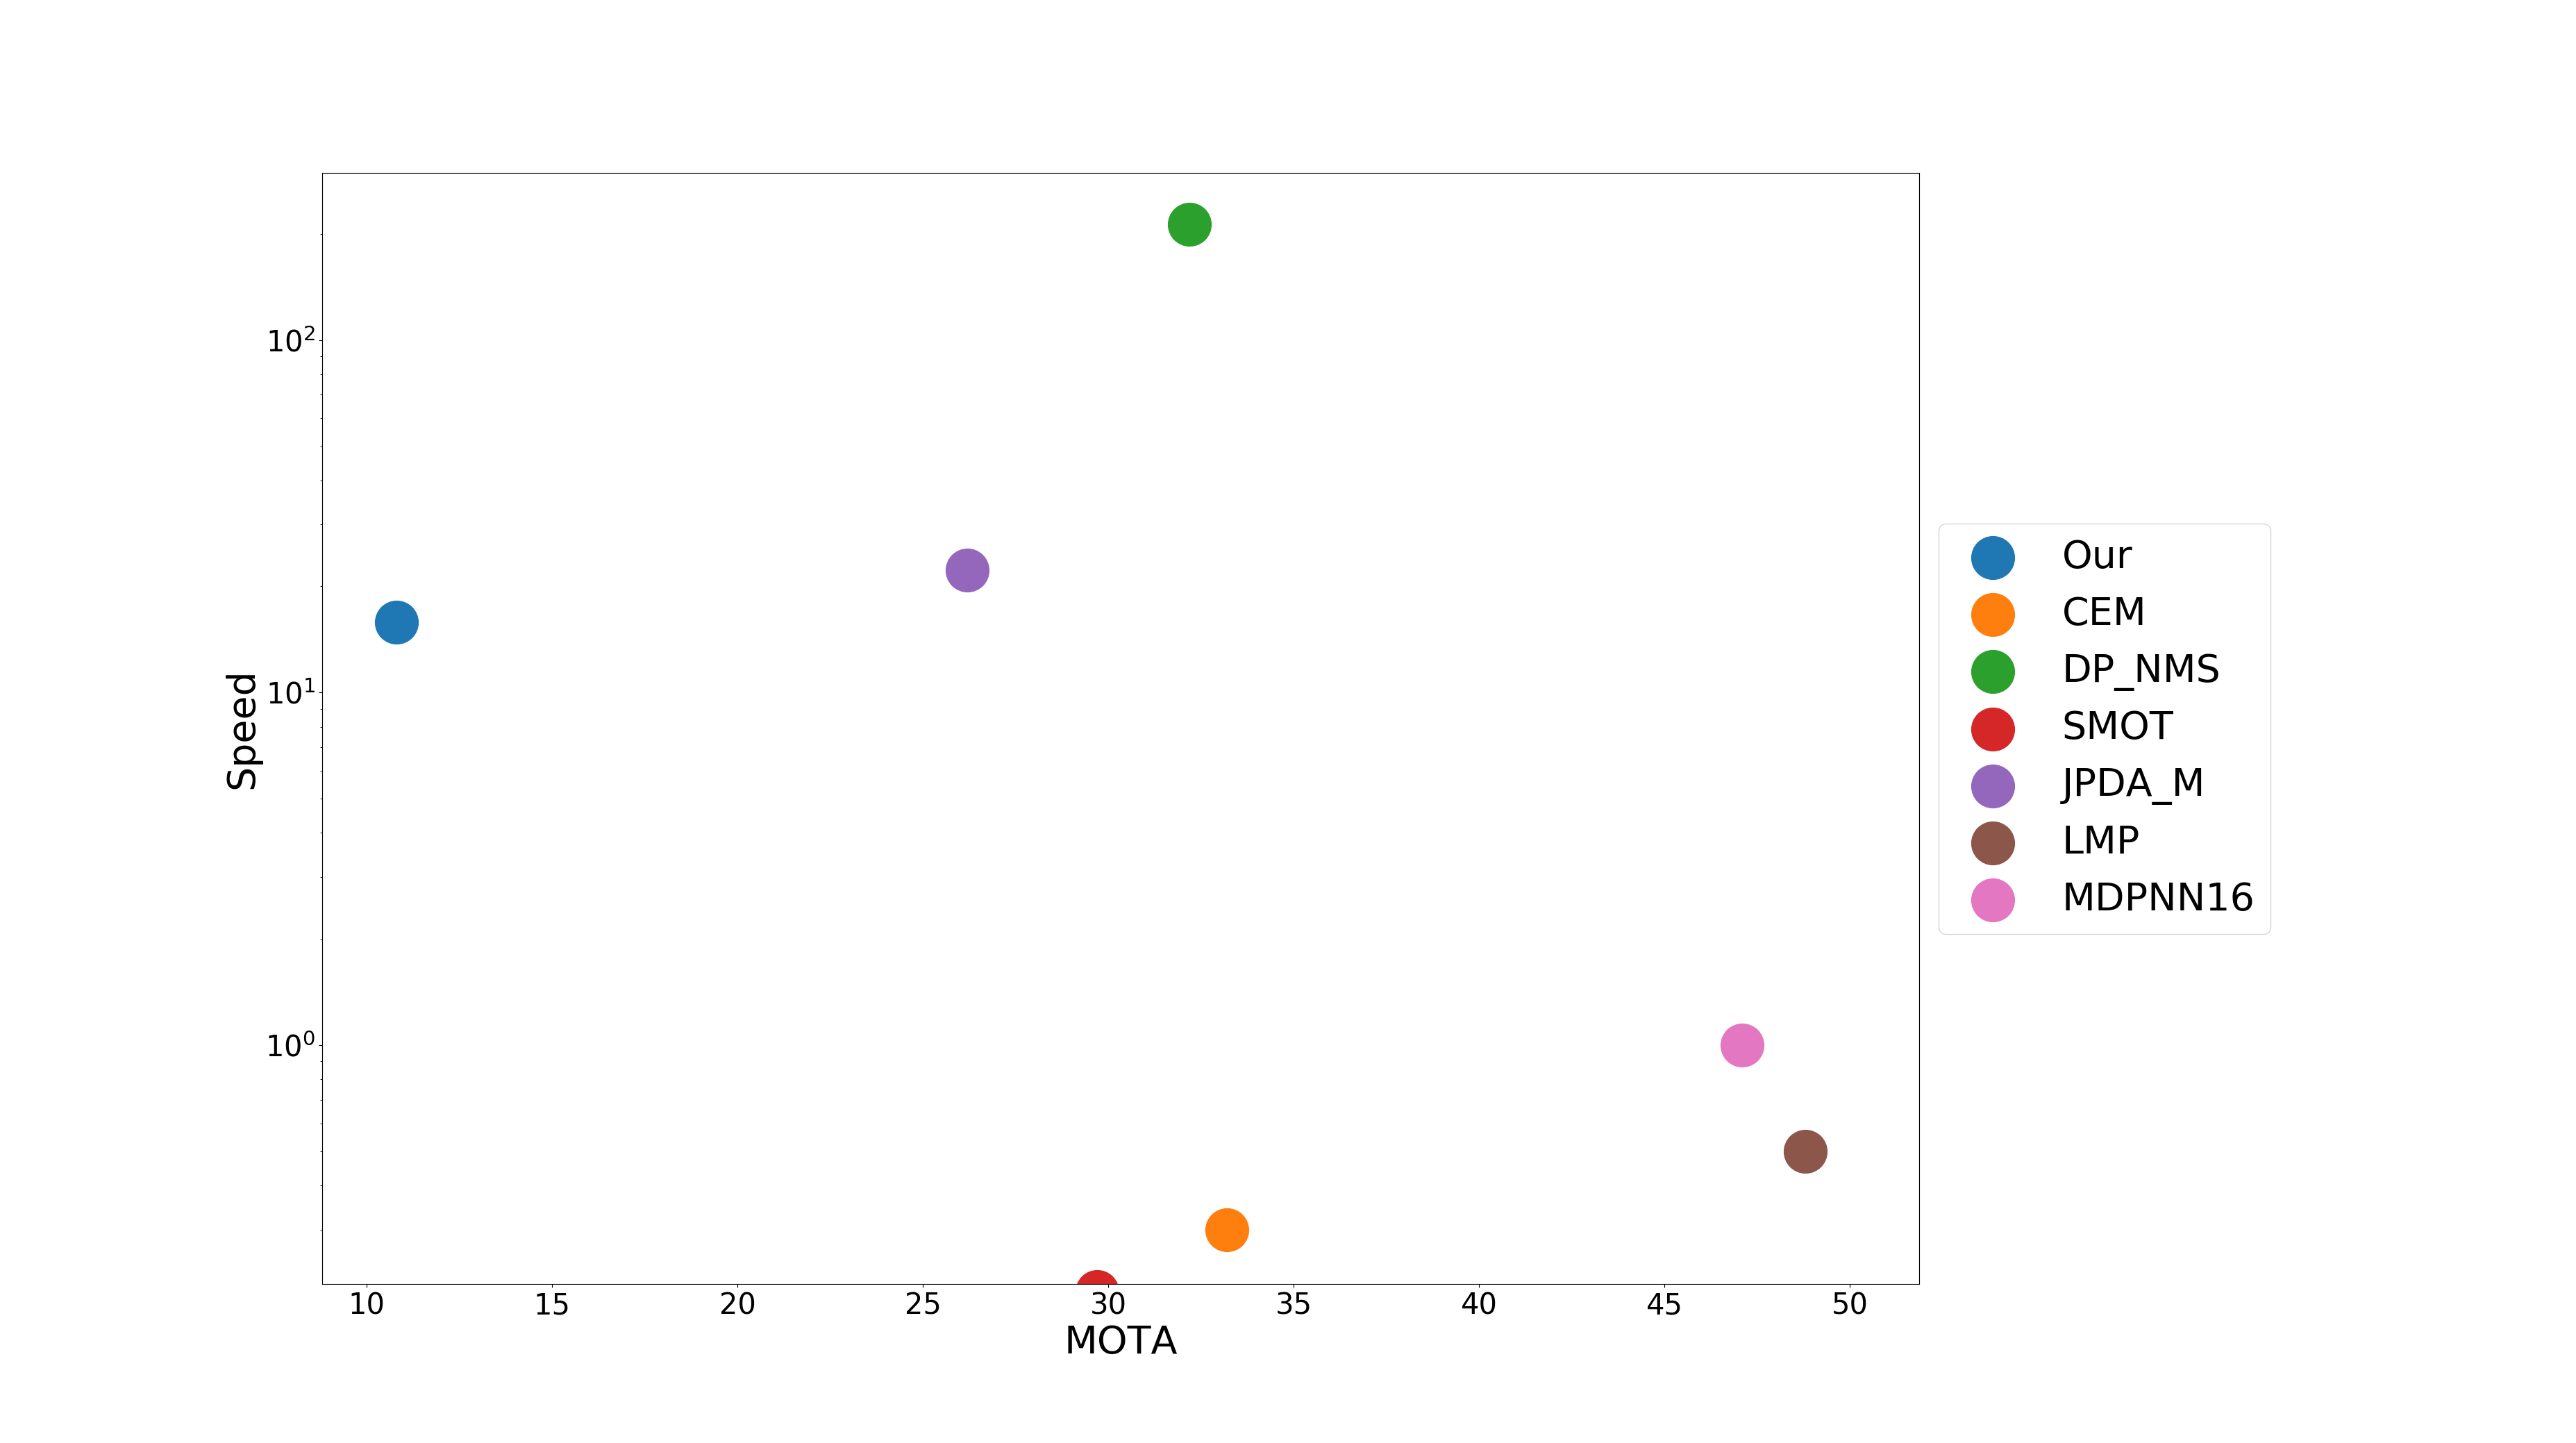
\includegraphics[width=16cm]{comparision/timeDAta.png}
\caption{Comparision with other algorithms.} \label{experimenComp}
\end{figure}




\section{Timing performance}\label{expeEVAL}


To analyse the timing performance of our algorithm we used the Town Centre sequence. We chose it because it has got a representative density of pedestrian. The mean frame rate of the algorithm with the person reidentification mechanism is $15.86$. In figure \ref{timing1} we can observe a barplot of time consumption and distribution of our algorithm per frame.  We notice the peaks each $30$ frames, these belong to the execution of the siamese network and it depends on how many blobs detections without assignment there are.

\begin{figure}[H]
\centering         
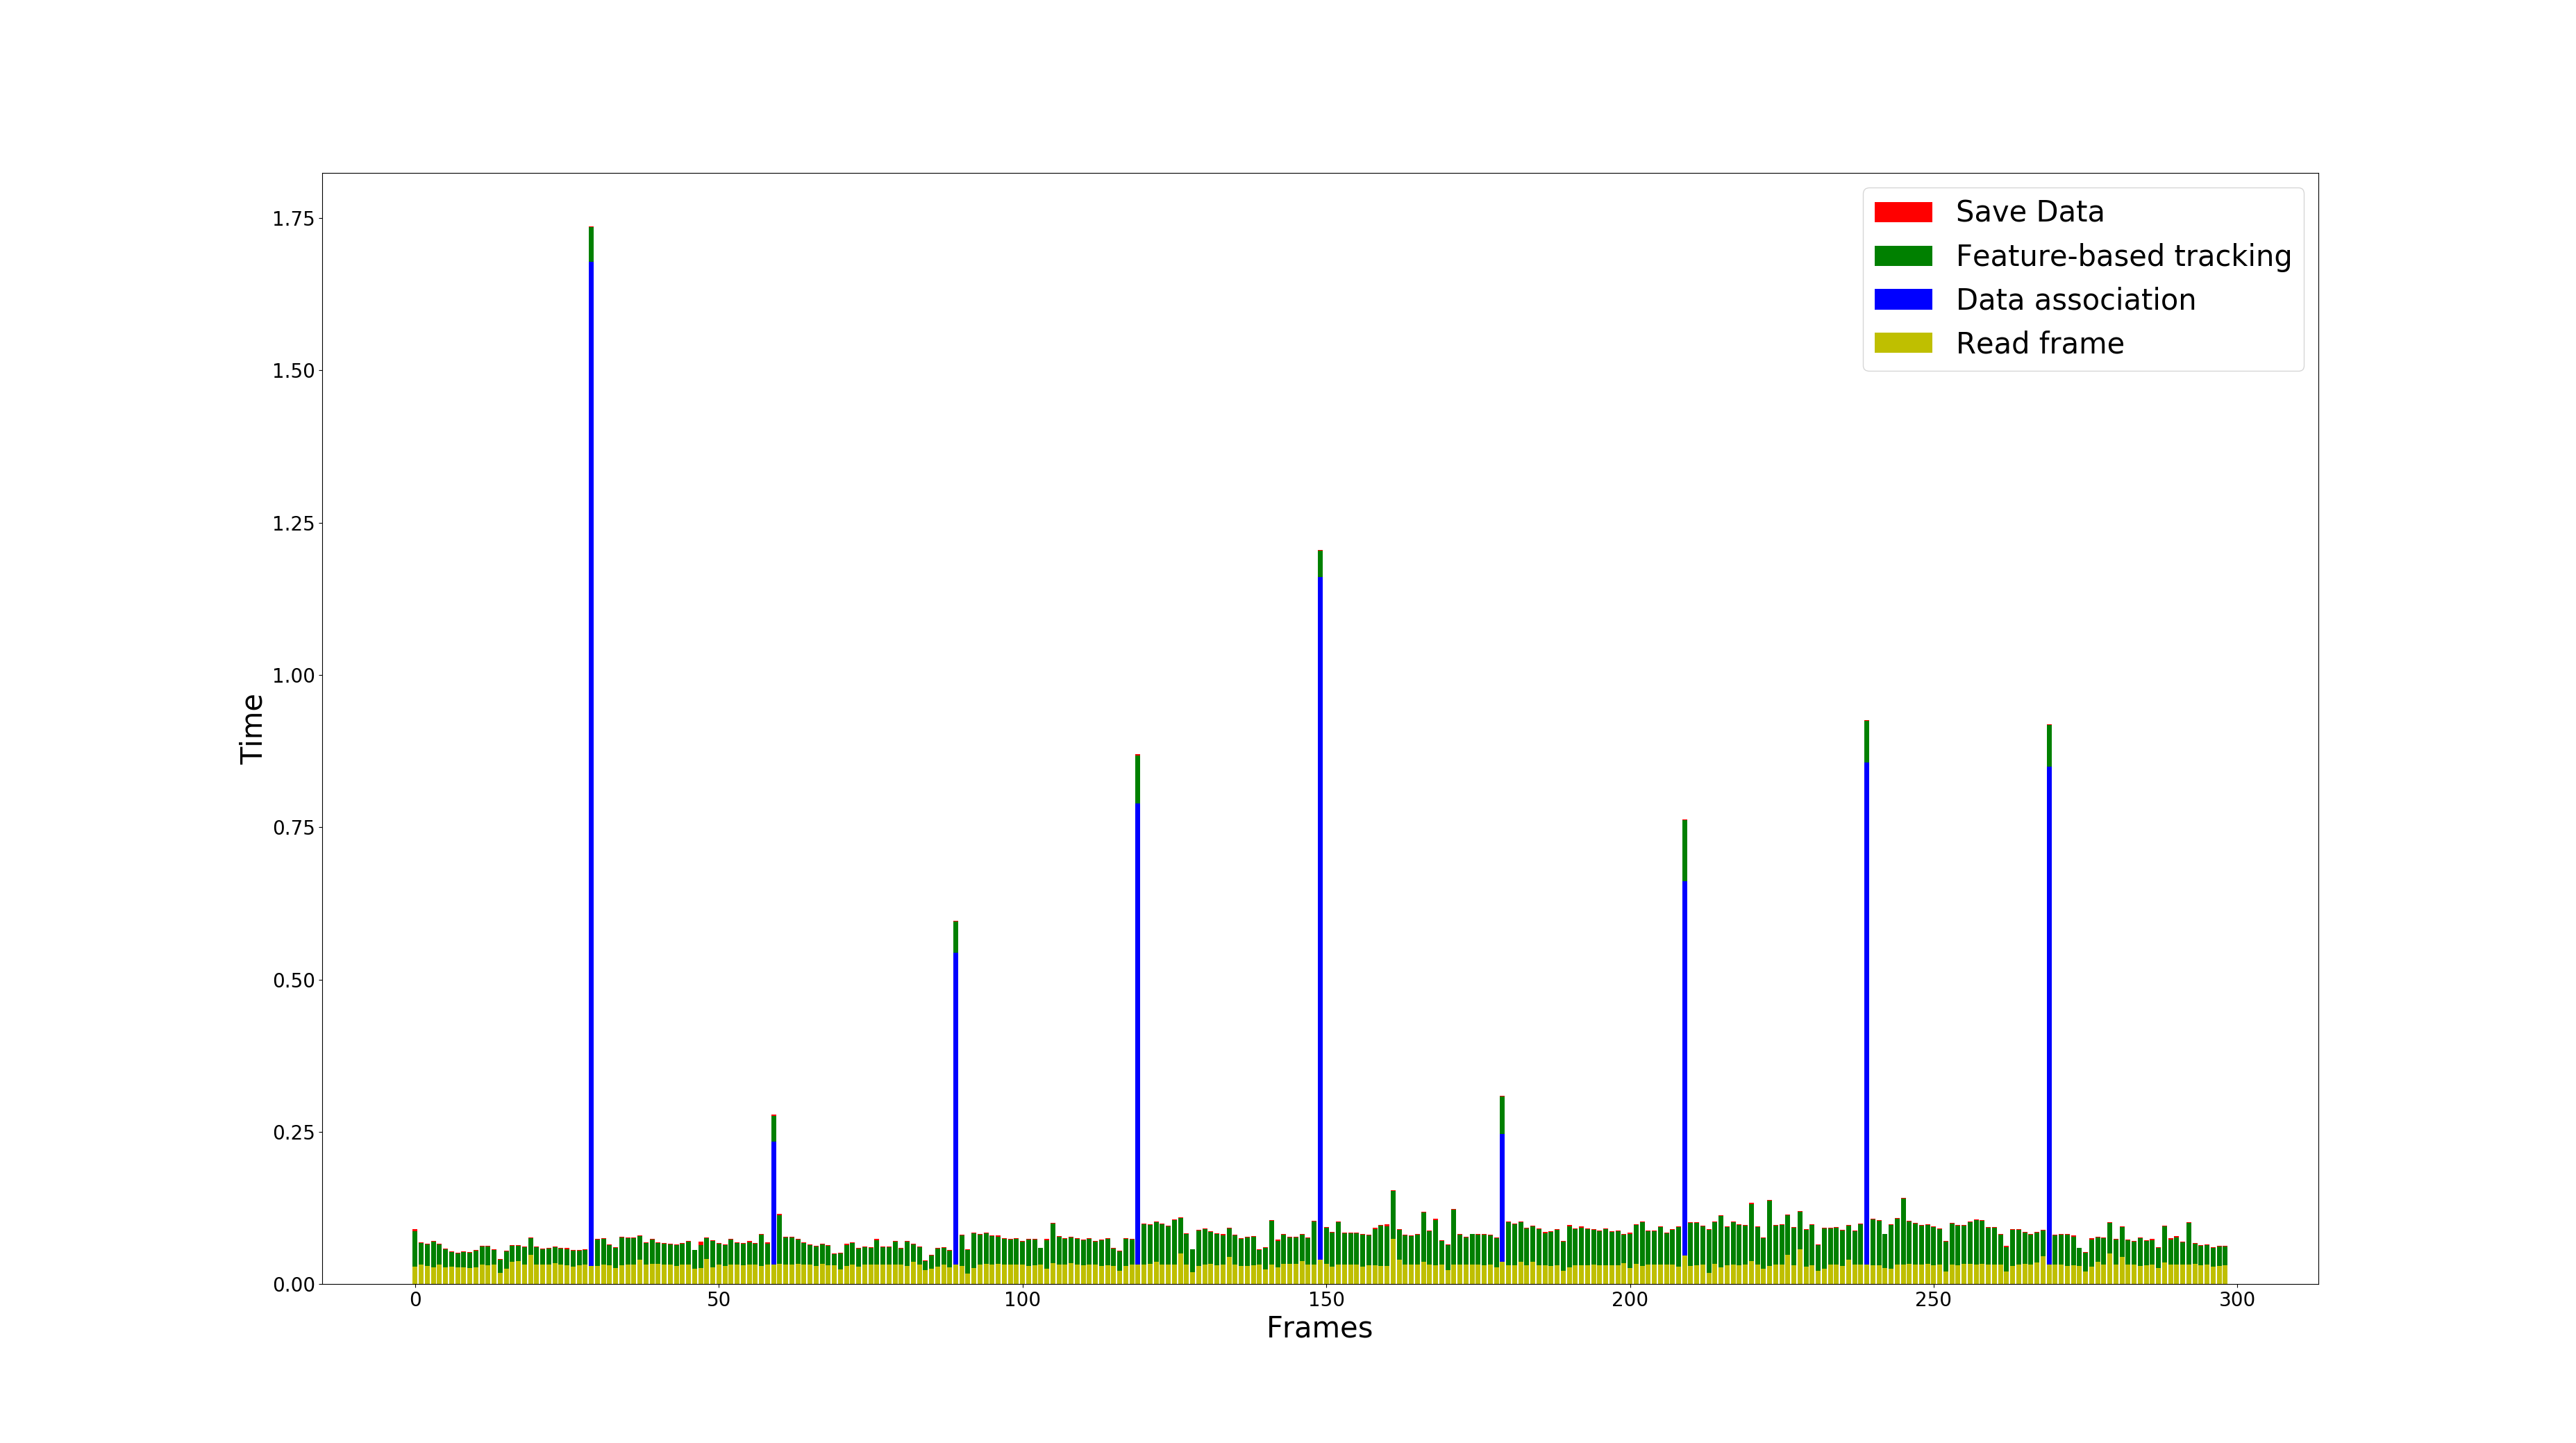
\includegraphics[width=0.9\linewidth]{graphicsRearrange/temps/figure4.png}
\caption{Barplot of the timming.} \label{timing1}
\end{figure}

Getting a zoom in the figure \ref{timing1}, we can sobserve the time of reading the frame remains constant. The feature-based tracking time distribution gets a peak every the detection and after that decreases due to erasing blobs with the lost mechanism and losing some feature points. The time for save the detections mantains costant and very small. 

\begin{figure}[H]
\centering         
\includegraphics[width=0.9\linewidth]{graphicsRearrange/temps/framezomm4.png}
\caption{Zoom in of the barplot.} \label{timing2}
\end{figure}



%To optimize our code we studied how to reduce the execution time of the tracking module, plotting the execution time against some dependent variables, in this case, the number of points and the size of the ROI, as we can observe in figure \ref{timing2}. We notice that the execution time is highly correlated with the size of the pedestrian's ROI and not with the number of points. The main responsible is the OpenCV's routine \texttt{calcOpticalFlowPyrLK()}, but we could not modify this parameter, and reducing the number of points would have a remarkable importance in the execution time. 
%
%


One we have analysed the global timing performance of our algorithm, we are going focus on the temporal evolution for different parameters of the feature-based tracking. The first of them it is the number of processing blobs. In the figure \ref{timing3} we observe an histogram of the number of blobs with their correspondant execution time. When more blobs process the tracking module it increases the time of their execution. The feature-based runs in a sequential way, with more blobs it increases the number of operations of the algorithm. 



\begin{figure}[H]
\centering         
\includegraphics[width=14cm]{jder/histogram_blobs.png}
\caption{Time histogram of number of blobs.} \label{timing3}
\end{figure}

Another parameter that we analysed it is the number of feature points that the feature-based tracking process. Increasing the number of feature points it also increases the execution time. We compute the displacement of each blob by the displacement of the features points, increasing the number of feature points, augments the execution time. 

\begin{figure}[H]
\centering         
\includegraphics[width=14cm]{jder/featruePoints.png}
\caption{Time histogram of feature points.} \label{timing4}
\end{figure}

Finally, the last parameter that we analysed it is the total blobs' area processed by the feature-based tracking. The execution time increase as increases the area of the blobs but at some point it reduces its rate of change.

\begin{figure}[H]
\centering         
\includegraphics[width=14cm]{jder/blobArea.png}
\caption{Time histogram number of area blob.} \label{timing5}
\end{figure}




